%%%%%%%%%%%%%%%%%%%%%%%%%%%%%%%%%%%%%%%%%%%%%%%%%%%%%%%%%%%%%%%%%%%%%%
% njuthesis 示例模板 v1.4.3 2025-05-21
% https://github.com/nju-lug/NJUThesis
%
% 贡献者
% Yu XIONG @atxy-blip   Yichen ZHAO @FengChendian
% Song GAO @myandeg     Chang MA @glatavento
% Yilun SUN @HermitSun  Yinfeng LIN @linyinfeng
% Yukai Chou @Muzimuzhi
%
% 许可证
% LaTeX Project Public License（版本 1.3c 或更高）
%%%%%%%%%%%%%%%%%%%%%%%%%%%%%%%%%%%%%%%%%%%%%%%%%%%%%%%%%%%%%%%%%%%%%%

%---------------------------------------------------------------------
% 一些提升使用体验的小技巧：
%   1. 请务必使用 UTF-8 编码编写和保存本文档
%   2. 请务必使用 XeLaTeX 或 LuaLaTeX 引擎进行编译
%   3. 不保证接口稳定，写作前一定要留意版本号
%   4. 以百分号(%)开头的内容为注释，可以随意删除
%---------------------------------------------------------------------

%---------------------------------------------------------------------
% 请先阅读使用手册：
% http://mirrors.ctan.org/macros/unicodetex/latex/njuthesis/njuthesis.pdf
%---------------------------------------------------------------------

\documentclass[
    % 模板选项(注意右端逗号)：
    %
    type = master, % 文档类型，默认为本科生
    degree = professional,        % 学位类型，默认为学术型
    %
    % nl-cover,   % 是否需要国家图书馆封面，默认关闭
    decl-page,  % 是否需要诚信承诺书或原创性声明，默认关闭
    %
    %   页面模式，详见手册说明
    % draft,                  % 开启草稿模式
    % anonymous,              % 开启盲审模式
    % minimal,                % 开启最小化模式
    %
    %   单双面模式，默认为适合印刷的双面模式
    % oneside,                % 单面模式，无空白页
    twoside,                % 双面模式，每一章从奇数页开始
    %
    %   字体设置，不填写则自动调用系统预装字体，详见手册
    fontset = fandol % |mac|macoffice|win|none,
  ]{njuthesis}

% 模板选项设置，包括个人信息、外观样式等

% 添加用户要求的格式设置
\usepackage{setspace}  % 用于设置行距

% 正文行距 1.5 倍已在 thesis-setup.def 中通过 \baselinestretch 统一设置，此处不再重复

% 设置脚注格式
% 脚注字号：小五号（\zihao{-5}，约 9pt）
\renewcommand{\footnotesize}{\zihao{-5}}
\renewcommand{\footnoterule}{\vspace*{-3pt}\hrule width 0.4\columnwidth height 0.4pt \vspace*{2.6pt}}

% 设置参考文献格式（在njuthesis.cls中已定义）
% 较为冗长且一般不需要反复修改，本研究把它放在单独的文件里
% njuthesis 参数设置文件 v1.4.3 2025-05-21

% 一些提醒：
%   1. \njusetup 内部千万不要有空行
%   2. 使用英文半角逗号(,)分隔选项
%   3. 等于号(=)两侧的空格会被忽略
%       3.1. 为避免歧义，请用花括号({})包裹内容
%   4. 本科生无需填写的项目已被特别标注
%   5. 可以尽情删除本注释

% info 类用于录入个人信息
%   带*号的为对应英文字段
\njusetup[info]{
    title = {信息激励与情感驱动：捐赠信息披露和社区讨论情感对比特币开源开发者活动的影响机制},
    % 中文题目
    % 直接填写标题就是自动换行
    % 可以使用换行控制符(\\)手动指定换行位置
    %
    title* = {Information Incentives and Emotional Drives: The Impact Mechanism of Donation Information Disclosure and Community Discussion Sentiment on Bitcoin Open-Source Developer Activity},
    % 英文题目
    %
    author = {冉红云},
    % 作者姓名
    %
    author* = {HongyunRan},
    % 作者英文姓名
    % 一般使用拼音
    %
    keywords = {比特币,开源社区,信息披露,开发者激励,开发者情感},
    % 中文关键词列表
    % 使用英文半角逗号(,)分隔
    %
    keywords* = {Bitcoin,{Open-Source Community},{Information Disclosure},{Developer Motivation},{Developer Sentiment}},
    % 英文关键词
    % 使用英文半角逗号(,)分隔
    %
    grade = {2023},
    % 年级
    %
    student-id = {522023140076},
    % 学号或工号
    % 研究生请斟酌大小写字母格式
    % 本模板并不会自动更正大小写
    %
    department = {信息管理学院},
    department* = {School of Information Management},
    % 院系
    %
    major = {图书情报},
    major* = {Library and Information Studies},
    % 专业
    %
    % major = {封面专业,摘要专业},
    % 研究生专业型学位可能遇到两处内容不一致的情况
    %
    supervisor = {颜嘉麒,教授},
    supervisor*= {JaqiYan,Professor},
    % 导师全称
    % 使用英文半角逗号(,)分隔中文姓名和职称
    %
    % supervisor-ii = {第二导师姓名,副教授},
    % supervisor-ii* = {Associate Professor My Second Supervisor},
    % 第二导师全称
    % 如果确实没有第二导师，不填写即可
    %
    submit-date = {2026-05-19},
    % 提交日期
    % 格式为 yyyy-mm-dd
    % 不填就是编译当天日期
    %
    %
    % 以下均为研究生项
    %
    % degree = {工程硕士},
    % degree* = {Master of Engineering},
    % 覆盖默认学位名称
    %
    field = {开源社区治理},
    field* = {Open source community developer incentives},
    % 研究领域
    %
    chairman = {康乐乐~教授},
    % 答辩委员会主席
    % 推荐使用波浪号(~)分隔姓名和职称
    %
    reviewer = {
        柯青~教授,
        赵月华~副教授
    },
    %
    % 答辩委员会成员
    % 一般为四名，使用英文半角逗号(,)分隔
    %
    clc = {G350},
    % 中国图书分类号
    %
    udc = {001.18},
    % 国际图书分类号
    %
    secret-level = {},
    % 密级
    %
    defend-date = {2026-05-24},
    % 答辩日期
    % 格式为 yyyy-mm-dd
    % 不填就是编译当天日期
    %
    email = {522023140076@smail.nju.edu.cn},
    % 电子邮箱地址
    % 只用于出版授权书
    %
    %
    % 以下用于国家图书馆封面
    confer-date = {2026-06-01},
    % 学位授予日期
    %
    bottom-date = {2026-06-01},
    % 封面底部日期
    %
    supervisor-contact = {
        南京大学~
        江苏省南京市栖霞区仙林大道163号
    },
    % 导师联系方式
}

% bib 类用于参考文献设置
\njusetup[bib]{
    resource = {thesis.bib},
    option = {
        sorting = gb7714-2015,
        gblanorder = englishahead,
    }
}

% image 类用于载入外置的图片
\njusetup[image]{
    % path = {{./figure/}{./image/}},
    % 图片搜索路径
    %
    % nju-emblem = {nju-emblem},
    % nju-name = {nju-name},
    % 校徽和校名图片路径
    % 建议使用 PDF 格式的矢量图
    % 使用外置图片有助于减少编译时间
    % 空置时会自动使用 njuvisual 宏包绘制
    %
    nju-emblem = {nju-emblem-purple},
    nju-name = {nju-name-purple},
    % 替换为紫色版本
    % 这个选项只能填写一次
    % 切换时要注释掉上方的黑色版本
}

% abstract 类用于设置摘要样式
\njusetup[abstract]{
    toc-entry = false,
    % 摘要是否显示在目录条目中
    %
    % underline = false,
    % 研究生英文摘要页条目内容是否添加下划线
    %
    % title-style = strict|centered|natural
    % 研究生摘要标题样式，详见手册
}

% 目录自身是否显示在目录条目中
\njusetup{
    % tableofcontents/toc-entry = false,
    % listoffigures/toc-entry   = false,
    % listoftables/toc-entry    = false
}

% 为目录中的章标题添加引导线
\njusetup[tableofcontents/dotline]{chapter}

% math 类用于设置数学符号样式，功能详见手册
\njusetup[math]{
    % style              = TeX|ISO|GB,
    % 整体风格，缺省值为国标（GB）
    % 相当于自动设置以下若干项
    %
    % integral           = upright|slanted,
    % integral-limits    = true|false,
    % less-than-or-equal = slanted|horizontal,
    % math-ellipsis      = centered|lower,
    % partial            = upright|italic,
    % real-part          = roman|fraktur,
    % vector             = boldfont|arrow,
    % uppercase-greek    = upright|italic
}

% theorem 类用于设置定理类环境样式，功能详见手册
\njusetup[theorem]{
    % define,
    % 默认创建内置的七种定理环境
    %
    % style         = remark,
    % header-font   = \sffamily \bfseries,
    % body-font     = \normalfont,
    % qed-symbol    = \ensuremath { \male },
    % counter       = section,
    % share-counter = true,
    % type          = {...},
    % define,
    % 以上设置项在重新调用 theorem/define 后生效
}

% footnote 类用于设置脚注样式，功能详见手册
\njusetup[footnote]{
  style = circled,
  % 使用圈码编号
  hang = false
}

% 页眉页脚内容设置
\njusetup{
  header/content = {
      {OR}{\rightmark},   % 奇数页页眉右侧：章名
      {OL}{},             % 奇数页页眉左侧：空
      {EL}{\leftmark},    % 偶数页页眉左侧：节名
      {ER}{}              % 偶数页页眉右侧：空
    },
  footer/content = {
      {C}{\thepage}       % 页脚居中：页码
    }
}

% 页眉页脚的字体样式
\njusetformat{header}{\small\kaishu}
\njusetformat{footer}{}

% 在盲审模式下隐藏学校信息
% \njusetup{anonymous-mode/no-nju}

% 一些灵活调整
% \njusetname{type}{本科毕业设计}                 % 我做的是毕业设计
% \njusetname{notation}{术语表}                   % 更改符号表名称
% \njusetlength{crulewd}{240pt}                   % 加长封面页下划线
% \njusetformat{subsection}{\normalfont\bfseries} % 修改 subsection 为小四号粗体宋体
% \njusetformat{tabular}{\zihao{-4}\bfseries}     % 修改表格环境的字号
% \EditInstance{nju}{u/cover/emblem-img}{align=l} % 左对齐的本科生封面校徽

% 根据用户要求添加的格式设置
% 1. 摘要格式设置
\njusetup[abstract]{
  title-style = centered,  % "摘要"二字居中
}

% 2. 正文标题格式设置
\njusetformat{chapter}{\centering\heiti\zihao{-2}\bfseries}  % 一级标题：黑体，小二，加粗，居中
\njusetformat{section}{\heiti\zihao{-3}\bfseries}            % 二级标题：黑体，小三，加粗
\njusetformat{subsection}{\heiti\zihao{4}\bfseries}          % 三级标题：黑体，四号，加粗

% 3. 正文格式设置
\renewcommand{\baselinestretch}{1.5}  % 1.5倍行距
\zihao{-4}\songti                     % 正文：小四号宋体

% 4. 脚注格式设置
\njusetup[footnote]{
  style = circled,
  hang = false
}

% 5. 参考文献格式设置（在biblatex中通过其他方式设置）
% \renewcommand{\bibfont}{\zihao{5}\songti}  % 五号字体，中文宋体，英文Times New Roman

% 6. 关键词格式设置（在abstract环境中自动处理）
% 7. 页码格式已在njuthesis.cls中设置（摘要罗马数字，正文阿拉伯数字）


% 解决 hyperref PDF 书签中的字体命令警告
\pdfstringdefDisableCommands{%
  \let\heiti\relax
  \let\songti\relax
  \let\kaishu\relax
  \let\zihao\relax
  \let\bfseries\relax
  \let\centering\relax
}

% 允许更宽松的断行，减少 overfull/underfull 警告
\sloppy

% 自行载入所需宏包
\usepackage{booktabs}    % 三线表（toprule/midrule/bottomrule）
\usepackage{tabularx}    % 自适应列宽表格
\usepackage{multirow}    % 跨行合并单元格
\usepackage{tikz}        % 绘制示意图
\usetikzlibrary{calc, positioning}
% \usepackage{subcaption} % 嵌套小幅图像，比 subfig 和 subfigure 更新更好
% \usepackage{siunitx} % 标准单位符号
% \usepackage{algorithm,algorithmic} % 展示算法伪代码

% CJK 字体回退：Fandol 缺失的生僻字使用 Noto Serif CJK SC
\newCJKfontfamily\notoserifjk{Noto Serif CJK SC}

% 在导言区随意定制所需命令
\NewDocumentCommand\todo{m}{\textbf{[待补充：#1]}} % 待填写标记

% 将 \cite 重定义为脚注引用（完整参考文献信息显示在页脚）
\AtBeginDocument{%
  \DeclareCiteCommand{\cite}[\mkbibfootnote]
    {\usebibmacro{prenote}}
    {\usedriver
      {\DeclareNameAlias{sortname}{default}}
      {\thefield{entrytype}}}
    {\multicitedelim}
    {\usebibmacro{postnote}}%
  
  % 参考文献格式：五号字体，单倍行距，悬挂缩进，两端对齐
  \AtBeginBibliography{%
    \renewcommand{\bibfont}{\zihao{5}\selectfont}%
    \setstretch{1.0}%
    \setlength{\bibitemsep}{0.3\baselineskip}%
    \setlength{\bibparsep}{0pt}%
  }%
}


\begin{document}

%---------------------------------------------------------------------
%   封面、摘要、目录
%---------------------------------------------------------------------

\maketitle
\raggedbottom

% 中文摘要
% 中文摘要
% 中文摘要
% 中文摘要
\begin{abstract}
比特币的开发完全依赖全球开源开发者的自愿贡献，激励其持续参与是核心治理挑战。
既有研究主要关注实际货币激励的效果，但驱动开发者行为的更深层力量可能是信息本身：
社区外部的捐赠公告凭借其携带的信号价值产生的激励效应，
社区内部的情感氛围在时间维度上对开发者行为走向的塑造作用，
以及两者之间从个体响应到社区传导的内在关联，这些问题尚缺乏系统考察。

本文以 GitHub 上的比特币开源项目为研究对象，以 Bitcoin Brink 基金会的两阶段捐赠信息披露
和社区 Issue 讨论情感为切入点，从外部到内部、从个体到社区逐层展开分析。
在个体层面，本文在剔除实际受资助开发者后，使用面板固定效应模型与工具变量方法，
识别捐赠信息披露的纯信息效应。
结果表明，非定向披露（X 平台捐款公告）与定向披露（官网受资助名单）均显著正向影响开发者的代码与审查活动，
但定向披露对非定向披露的正向效应产生负向调节，印证了期望失验理论所预测的失望机制。
在此基础上，本文将视线转向社区层面，采用向量自回归（VAR）模型考察 Issue 讨论情感对开发活动的动态传导。
发现滞后一期的负面情感正向影响代码与讨论活动，而代码活动在滞后两期负向影响讨论活动，
揭示了情感经由代码和讨论活动再传导至讨论活动的动态路径，
分别以情感即信息理论和目标手段替代理论获得解释。
两项研究共同表明，在开源社区中信息在金钱之外独立驱动着开发者的行为决策，外部捐赠信号与内部情感信号分别从个体激励响应和社区动态传导两个层面，共同构成了信息驱动参与的完整图景。
本文的研究发现为开源社区的治理策略和基金会的信息披露设计提供了实证参考。
\end{abstract}

% 英文摘要
\begin{abstract*}
Bitcoin's development relies entirely on voluntary contributions from open-source developers worldwide, making sustained participation a central governance challenge. While prior research has focused on the effects of monetary incentives, a more fundamental force, information itself, remains underexamined: whether external donation announcements can motivate developers solely through the signals they carry, how the affective climate generated within community discussions dynamically shapes developer behavior, and whether individual responses and community-level dynamics are intrinsically linked.

This thesis addresses these questions using the Bitcoin GitHub repository as the empirical context, taking Bitcoin Brink's two-stage donation disclosure and community Issue discussion sentiment as entry points, progressing from external to internal information sources and from individual to community levels of analysis. At the individual level, after excluding actual grantees to isolate pure information effects, panel fixed-effects and instrumental variable models reveal that both untargeted disclosures (donation announcements on X) and targeted disclosures (grantee lists on Brink's website) significantly increase code and review activities, while targeted disclosure negatively moderates the positive effect of untargeted disclosure, consistent with expectancy disconfirmation theory. Building on these findings, the thesis moves to the community level, employing vector autoregression (VAR) to examine how Issue discussion sentiment transmits across time. Results show that lagged negative sentiment positively influences both code and discussion activities, while lagged code activity suppresses subsequent discussion activity, revealing a dynamic pathway from sentiment through code and discussion activities, explained respectively by affect-as-information theory and goal-means substitution theory. Together, the two studies demonstrate that in open-source communities, information independently drives developer behavior beyond monetary incentives: individual-level incentive responses and community-level dynamic transmission collectively form a complete picture of information-driven participation. These findings offer actionable insights for open-source governance and foundation disclosure strategy design.
\end{abstract*}

% 目录
\tableofcontents
% 图表目录
\listoffigures
\listoftables

%---------------------------------------------------------------------
%   正文
%---------------------------------------------------------------------
\mainmatter

%%====================================================================
\chapter{绪论}
%%====================================================================

\section{研究背景}

过去数十年间，开源软件（Open-Source Software，OSS）已从小众的技术运动成长为
现代数字基础设施不可或缺的组成部分\cite{lerner2002simple,chen2021opensource}。
Linux 操作系统支撑着全球绝大多数服务器与移动设备，
Apache HTTP Server 托管着互联网上数量庞大的网站，
Python、Git 等工具深度嵌入全球数百万开发者的日常工作流程，
这些广为人知的软件均是开源模式下协作开发的产物\cite{lakhani2003open}。
与商业软件的封闭开发不同，开源项目以源代码公开、全球开放协作为基本特征，
任何人均可查看代码、提交改进、报告问题，无需与项目组织存在任何雇佣关系。
这种模式极大地降低了知识传播的门槛，形成了高度去中心化的创新生态；
与此同时，也带来了一个根本性的挑战：既然贡献是自愿的，
理解驱使开发者持续投入时间和精力的因素便成为开源研究的核心议题。

这一问题在比特币（Bitcoin）社区中表现得尤为突出。
比特币是 Satoshi Nakamoto\footnote{Satoshi Nakamoto 为化名，其真实身份至今未被确认。} 于2008年提出的点对点电子现金系统\cite{nakamoto2008bitcoin,cheng2024bitcoin}，
其底层协议自诞生伊始便以完全开源的形式运作，
项目代码库托管于 GitHub\footnote{GitHub（\url{https://github.com}）是全球最大的代码托管与开源协作平台，由微软于2018年收购。} 平台，目前已积累超过76,000名关注者，
吸引了来自全球的数千名开发者贡献代码与文档。
比特币不同于其他开源项目的关键在于：它背后没有任何公司主体为开发活动提供资金保障，
也没有雇主为核心开发者发放薪酬。整个项目的存续与演进完全建立在志愿贡献的基础之上，
而这些贡献直接关系到价值数千亿美元的金融网络的安全性与可靠性。
一旦核心开发者离去或社区贡献萎缩，比特币网络将面临严峻的技术维护风险。
在此背景下，如何有效激励开发者持续贡献，已成为比特币社区乃至整个开源生态的核心治理议题。

学术界对开源开发者激励机制的研究已积累了丰富成果。
早期研究发现，开发者的参与主要由内在动机驱动，包括对技术问题的纯粹兴趣\cite{shah2006motivation}、在同行社区中积累声誉的渴望\cite{lerner2002simple}，以及通过贡献提升个人技能以获得更好职业机会的考量\cite{fang2009understanding}。这些因素共同构成了开发者持续投入的基础动力\cite{nov2007motivates}。
此外，Davidson 等人\cite{davidson2014older}指出，利他精神与自我实现感同样是重要的内在激励来源。
这些研究共同刻画了一个图景：在开源生态中，
开发者的自主性与社区归属感往往是持续贡献的核心支撑\cite{wang2023config}，
而非来自外部的物质回报。

然而，随着开源软件在商业和社会中的重要性持续上升，
外部经济激励机制也开始进入研究者的视野。
货币奖励被证明能够在一定程度上促进开发者的贡献\cite{wang2022monetary}，
但其与内在动机的关系颇为微妙：若管理不当，不适当的金钱激励反而可能产生挤出效应，
削弱开发者原本的内在驱动力\cite{benabou2003intrinsic,qiao2021mitigating}。
2019年，GitHub 正式推出 Sponsors 机制\footnote{GitHub Sponsors：\url{https://github.com/sponsors}，允许用户直接向开源开发者提供定期或一次性经济赞助。}，首次为开源贡献提供了平台级的捐赠基础设施，
使任何人都可以向自己欣赏的开发者提供经济支持。
这一机制的出现引发了学界的广泛关注。
Shimada 等人\cite{shimada2022github}的研究发现，
部分开发者将赞助本身视为一种新型的社区贡献方式；
Zhang 等人\cite{zhang2022who}进一步揭示，赞助在短期内对开发活动具有温和的正向效应，
但获得赞助的可能性与开发者在社区中的社会地位密切相关；
Conti 等人\cite{conti2023incentivizing}则通过更长期的追踪研究发现，
实际收到赞助反而可能对创新活动产生长期负向影响，
这与挤出效应的理论预测相吻合。
Overney 等人\cite{overney2020not}的研究也表明，
单纯依靠捐赠机制提升开源贡献的效果并不显著，
暗示捐赠的效用可能远比表面看起来复杂。

上述研究的密集出现，折射出开源生态在现实层面所面临的深层可持续性困境。
现代数字经济的高速运转建立在大量关键开源组件之上，然而这些组件的维护工作往往
高度集中于少数志愿开发者，缺乏稳定的制度性支持。
2021年底曝光的 Apache Log4j 漏洞事件\footnote{即 CVE-2021-44228，又称Log4Shell，被评为 CVSS 最高危险等级10.0分，影响了全球数十亿台设备。}以极具冲击力的方式揭示了这一隐忧：
一个嵌入全球数十亿软件系统的核心日志库，长期仅由数名志愿者以业余时间维护，
其安全漏洞的存在几乎使整个互联网基础设施陷入系统性风险\cite{alami2024sustainability}。
在比特币生态中，这种脆弱性以更为独特的方式呈现：
比特币网络目前承载着超过万亿美元规模的资产，
而其底层协议的核心维护工作却高度依赖为数不多的全职开发者，
任何核心人才的流失或社区参与的持续萎缩，
都均可能对协议的演进能力乃至网络的整体安全构成深远威胁。
正是在这一背景下，以 Brink\footnote{Bitcoin Brink 官方网站：\url{https://brink.dev}。} 为代表的专项资助机构应运而生，
探索出基于信息透明化和分阶段披露的独特激励路径，
以期在不违背去中心化治理理念的前提下，维持广大开发者群体的参与意愿与贡献活力\cite{wu2024governance}。
对这一机制的科学评估，因此具有超越单一案例的现实普遍意义。

综合上述研究可以发现，现有文献对捐赠的理解主要集中于其作为货币转移的经济效应，
即货币激励能否直接促进开发者参与这一层面。
然而，在实际的捐赠生态中，信息的流动往往先于资金的转移，
而且覆盖的受众也远比实际受益者更广。
当一个资助机构在社交媒体上宣布收到了一笔捐款时，
所有关注该机构的开发者都会接收到这条信息，
无论他们最终是否能从中受益。这条信息本身能否对其行为产生可测量的影响，
目前尚缺乏实证检验。这种仅凭信息而非实际资金转移的激励效应，
在既有文献中几乎没有得到系统性的研究。
这一研究空白尤为值得关注，因为信息披露相较于实际资金分配具有近乎为零的边际成本，
同时又能触达整个社区而非少数受资助者，
若其激励效应确实存在，则将为开源社区的低成本治理提供重要的政策工具。
从信息经济学的视角审视，捐赠公告的本质是一种信号传递行为，
它向潜在贡献者同时传递了项目获得外部认可、机构具备奖励意愿以及未来可获得回报等多重信号，
这些信号会在开发者心中激活或调整预期结构，进而影响其参与决策\cite{connelly2011signaling}。
类似的逻辑在众筹研究中已有部分印证：项目进展公告能够显著提升后续的支持率，
即便公告内容并不伴随任何即时的经济转移\cite{mollick2014dynamics}。
然而，在开源开发者群体中，信息披露能否通过类似机制引发可测量的行为变化，
尤其是不同类型披露（普惠型与定向型）是否产生差异化效应，
目前在实证层面仍是空白。

与此同时，在社区内部的信息维度上，同样存在一个亟待填补的研究空白。
开源项目的 Issue 讨论区不仅是技术问题协商的场所，
也是社区成员情感状态汇聚与传导的媒介。
当项目遭遇重大 Bug、核心功能争议或对外部环境变化的集体焦虑时，
Issue 区的讨论情感会随之出现明显的极性变化。
Guzzi 等人\cite{guzzi2013}发现，开源社区的协作沟通中蕴含着丰富的情感信息，
这些信息构成了社区健康状态的重要信号。
然而，社区情感如何在时间维度上影响开发者的具体行为，
情感变化是否能够预测随后的代码活动或讨论活动，
以及不同类型的开发活动之间是否存在相互促进或相互抑制的动态关系，
目前尚缺乏系统性的实证探讨。
现有将情感分析引入开源社区的研究，大多以描述情感分布的静态特征
或考察情感与代码质量的截面相关性为主要目标\cite{guzzi2013}，
较少采用动态因果推断框架，系统地检验情感冲击在时间轴上如何传导至开发者的行动决策。
更重要的是，代码活动与讨论活动之间的动态互动（即
当开发者通过编写代码回应社区问题时，是否会相应地减少讨论参与，
形成活动层面的替代关系）这一机制既有理论依据，
又对理解开源社区的协作动态具有重要意义，
却在实证研究中几乎未曾得到正面检验。
在信息行为研究的视角下，情感本身就是一种重要的信息资源，
它向社区成员传递项目状态的信号，影响其行动意愿与行动方向。
从这一视角出发理解开发者行为，有可能揭示出超越个体激励机制的社区层面动态规律。

正是在上述背景下，本研究将视线转向比特币开源社区，
尝试从信息视角对上述两个研究空白进行系统性的实证回应。

\section{研究场景：比特币社区与 Brink 基金会}

比特币开源社区为本研究提供了几乎难以在其他情境中复现的理想研究场景，
核心原因在于一个独特的研究对象：非盈利组织 Bitcoin Brink（以下简称Brink）
及其所形成的两阶段捐赠信息披露机制。

Brink 成立于2020年，是目前规模最大的专注于比特币核心协议开发的资助机构，
采用众筹模式面向个人捐赠者和机构投资者募集资金，
并通过严格的申请审核流程为符合条件的比特币开发者提供全职工作资助。
由于比特币本身的去中心化哲学，Brink 刻意保持独立的非盈利定位\cite{riehle2010economic}，
其资金来源和资助决策均对外公开，以维护社区信任。
正是这种对透明度的高度重视，催生了一套具有内在研究价值的两阶段信息披露机制。

第一阶段，当 Brink 收到捐款时，会在其 X 平台（原 Twitter）官方账号上发布公告，
公开感谢捐赠方并注明捐款金额，但不说明这笔资金将用于资助哪位具体的开发者。
这类公告面向所有关注者广泛传播，每一位比特币开发者都可能看到这条信息；
由于受益人尚未确定，公告中所传递的核心信号是这个社区正在获得外部支持，
有资金可以用于奖励开发者。本研究将这类披露定义为非定向披露（Untargeted Disclosure），
强调其普惠性，即每位开发者均可合理地将自己视为潜在受益者。
第二阶段，经过通常为数周乃至数月的申请与审核流程后，
Brink 会在其官方网站上正式宣布当期受资助开发者名单，
列出姓名、资助金额及资助期限，并对其贡献做出肯定性说明。
与第一阶段不同，这类披露所传递的核心信号是谁因为贡献突出而获得了认可与资金支持。
本研究将其定义为定向披露（Targeted Disclosure），
因为它指向具体的个人，对于未入选者而言也意味着明确的排除。

两次披露在时间上相互分离、在内容上存在本质差异，
这在方法论层面具有重要价值：研究者得以将两种信息效应分别识别，
而无需将其与实际资金的到达相混淆。
更重要的是，在本研究的观测期内（2022年1月至2023年12月），
Brink 实际资助的开发者数量极为有限，两年内仅资助了8名开发者转为全职从事比特币开发。
这意味着，通过将这8名实际受资助者从分析样本中剔除，
研究者可以专注于研究对于其余1610名开发者而言，
捐赠信息的公开本身（而非任何真实的金钱转移）
是否对其活动行为产生了可测量的影响。
这种信息与金钱的干净分离，在开源捐赠研究中极为罕见，
构成了本研究得以回答核心问题的关键条件。

除了捐赠信息披露机制之外，比特币社区还具备另一项研究优势：
完整、开放且可系统处理的 Issue 讨论历史。
比特币项目自创立以来积累了大量的 Issue 记录，
涵盖 Bug 报告、功能讨论、安全议题乃至社区内部的技术争论，
这些文本构成了追踪社区情感动态变化的完整语料库。
结合 GH Archive 对 GitHub 活动数据的完整记录、X 平台的公告历史、
Brink 官网的资助档案以及 Google Trends 的搜索量数据，
本研究得以在同一社区中、围绕同一组开发者群体，
同时探讨外部信息与内部情感两个维度对开发者行为的影响。
数据来源的多元性与可靠性，是本研究最终选择比特币社区作为研究对象的重要原因。

需要明确的是，本研究聚焦于比特币这一单一开源项目。
与多项目横向比较或跨社区大规模分析的研究范式不同，
本研究的分析框架以单一项目内部的纵向变异为核心识别来源，
所有实证结论均建立在比特币核心仓库的开发者活动数据与 Brink 基金会的信息披露时间序列之上。
选择单一项目研究设计的优势在于：可以通过对项目历史、社区规范和制度背景的深入理解，
建立更为精确的因果识别条件（如剔除实际受助开发者以分离信息效应与货币效应），
从而在内部效度上获得更大保障。
这一设计选择同时也意味着，本研究的实证结论在推广至其他开源项目时需保持审慎。
不同项目在技术架构、社区规模、协作规范、资金模式和文化价值观等方面存在显著差异，
这些差异可能调节信息披露的激励效应强度乃至方向。
后续研究可在更多样化的开源项目（如不同编程语言生态、不同治理结构的项目、
不同规模社区的基金会）中对本研究的核心发现进行复现与扩展，
以检验理论的外部效度和边界条件。


\begin{figure}[htbp]
    \centering
    \begin{tikzpicture}[
        node distance=0.8cm and 2.6cm,
        box/.style={rectangle, draw=black, rounded corners=2pt,
                    minimum width=2.0cm, minimum height=0.6cm,
                    align=center, font=\small, inner sep=6pt},
        cbox/.style={box, fill=black!5},
        arrow/.style={->, >=stealth, thick},
    ]
    % 中心：Brink 基金会
    \node[cbox, minimum width=2.4cm, minimum height=2.0cm] (brink) {Brink\\基金会};

    % 左上：捐赠方
    \node[cbox, above left=1.4cm and 2.6cm of brink] (donor) {捐赠方};
    % 右上：X 平台
    \node[cbox, above right=1.4cm and 2.6cm of brink] (x) {X 平台};
    % 左下：开发者
    \node[cbox, below left=1.4cm and 2.6cm of brink] (dev) {开发者};
    % 右下：官网
    \node[cbox, below right=1.4cm and 2.6cm of brink] (web) {官网};

    % 阶段一（上方）
    \draw[arrow] (donor.east) to node[above, font=\small] {资金捐赠} (brink.north west);
    \draw[arrow] (brink.north east) to node[above, font=\small] {披露捐款信息} (x.west);
    \node[font=\small\bfseries, above=0.2cm of donor.north west, anchor=south west] {阶段一：非定向披露};

    % 阶段二（下方）
    \draw[arrow] (dev.east) to node[below, font=\small] {申请资助} (brink.south west);
    \draw[arrow] (brink.south east) to node[below, font=\small] {公布受资助名单} (web.west);
    \node[font=\small\bfseries, below=0.2cm of dev.south west, anchor=north west] {阶段二：定向披露};

    \end{tikzpicture}
    \caption{Brink 捐赠信息披露流程}
    \label{fig:brink-flow}
\end{figure}

\subsection{非定向披露的运作机制}

在 Brink 的日常运营中，每当完成一笔捐款的接收与确认，便会在其官方 X（原 Twitter）账号 @bitcoinbrink 发布捐赠公告。公告内容通常包含捐赠方名称、捐款金额以及对捐赠方的公开致谢，但不涉及任何资金用途的具体说明，即无法从公告中判断该笔资金将最终资助哪位或哪几位开发者。在本研究观测期（2022年1月至2023年12月）内，Brink 共发布此类非定向披露公告19次，其中15次明确披露了具体捐款金额，单笔披露金额从数千美元到500万美元不等，显示出相当大的跨期变动幅度。非定向披露的典型形式为 X 平台上的一段简短推文，通常包含如下要素：捐赠方名称或代号、捐款金额（以美元或比特币计）、对捐赠方的公开致谢语，以及 Brink 对持续推动比特币核心开发的承诺声明。这类推文的信息密度较低，内容高度标准化，不包含任何关于具体资助用途或受助候选人的信息。图~\ref{fig:untargeted-example} 展示了一条典型的非定向披露推文，其中 Brink 宣布收到来自 @jack 与 \#startsmall 的500万美元捐款承诺，公告仅涉及捐款金额和致谢，未说明资金将定向资助任何特定开发者。

\begin{figure}[htbp]
    \centering
    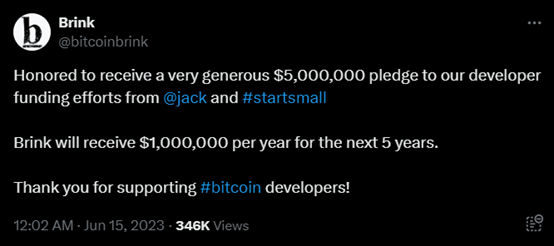
\includegraphics[width=0.72\textwidth]{figures/untargeted_example.png}
    \caption{非定向披露示例：Brink X 平台捐款公告（2023年6月15日）}
    \label{fig:untargeted-example}
\end{figure}

从信息传播路径来看，X 平台的公告面向所有公开关注者，不区分身份与贡献层级。这意味着在 Brink 生态中从事开发工作的1600余名开发者，均有机会在第一时间获取这一信息。由于公告并未指定受益方，每位开发者在接收到有大额捐款注入的信息时，都可以合理地将自己纳入未来受益者的范畴。Kobayakawa 等（2020）\cite{kobayakawa2020impact} 的研究表明，加密货币市场的资本规模与开源开发活动之间存在正向关联，而 Brink 的捐款公告正是将加密货币生态的资本流动与开源开发者的激励感知直接联结起来的传播节点。这种普惠性信息结构，正是非定向披露区别于其他激励机制的核心特征。

从期望理论的视角来看，非定向披露事件至少通过两条心理路径影响开发者的行为意愿：其一是效价路径，捐款公告向外界传递了Brink掌握充足资金且有能力对更多开发者给予资助的积极信号，提升了开发者对潜在奖励价值的主观评估；其二是期望路径，公告所释放的资金实力信号强化了开发者对当前活动能够获得回报的信心。综合来看，非定向披露通过激活开发者的积极期望状态，有望在短期内促进活动参与的增加。这一机制在实质上类似于众筹平台上的资金积累公示效应：Wang 等（2022）\cite{wang2022monetary} 在分析货币激励与知识溢出的研究中指出，公开的资金规模信息能够通过期望路径有效激励潜在贡献者的参与投入。

\subsection{定向披露的运作机制}

与非定向披露不同，定向披露发生在 Brink 完成内部审核并正式确定受资助开发者之后。Brink 通过在其官方网站（\url{https://brink.dev}）更新受资助者页面，公开列出获批开发者的 GitHub 用户名、资助开始时间及资助期限。这类披露具有明确的指向性：信息内容从捐款来源与金额转变为受资助者的具体身份，标志着抽象的激励预期转化为可观察的分配事实。

在本研究的观测窗口内，Brink 共进行了5次定向披露，受资助开发者及公告时间汇总如表~\ref{tab:grantees} 所示。

\begin{table}[htbp]
    \centering
    \small
    \caption{Brink 受资助开发者名单（2022年1月—2023年12月）}
    \label{tab:grantees}
    \begin{tabularx}{\textwidth}{p{2.8cm}Xp{4.5cm}}
        \toprule
        披露日期 & 受资助开发者（GitHub 用户名） & 说明 \\
        \midrule
        2022年4月4日  & 0xB10C、vincenzopalazzo、dergoegge、brunoerg & 本轮共资助4名开发者，规模最大 \\
        2022年5月13日 & fanquake & 单独资助 \\
        2022年6月30日 & adiabat   & 单独资助 \\
        2022年7月29日 & stickies-v & 单独资助 \\
        2023年5月4日  & fjahr      & 单独资助 \\
        \bottomrule
    \end{tabularx}
\end{table}

图~\ref{fig:targeted-example} 展示了规模最大的一次定向披露（2022年4月4日）的官方公告页面截图，Brink 明确列出了4名获批开发者的姓名及其比特币开发背景，信息的指向性与权威性与非定向披露截然不同。

\begin{figure}[htbp]
    \centering
    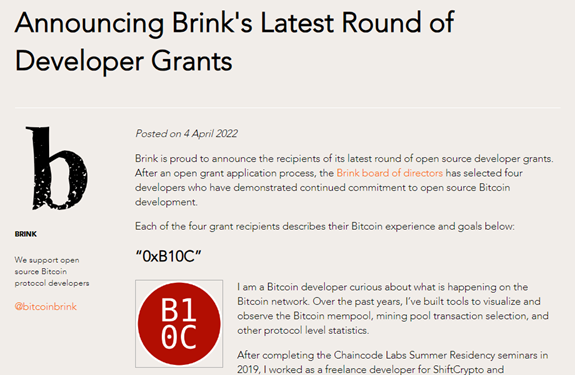
\includegraphics[width=0.72\textwidth]{figures/targeted_example.png}
    \caption{定向披露示例：Brink 官网受资助名单公告（2022年4月4日）}
    \label{fig:targeted-example}
\end{figure}

从期望理论的工具性维度分析，定向披露为非受助开发者提供了一个具体的参照：他们能够看到哪类贡献者（以代码技能见长、常年深耕核心协议）最终获得了资助，由此推断自身活动与奖励之间的因果关联是真实存在的，进而形成只要持续高质量参与，也有机会进入下一轮资助名单的工具性预期。这一机制有别于非定向披露的效价驱动，而是通过直接示范绩效—奖励路径，强化开发者的努力意愿。

然而，定向披露的排他性也具有两面性。在公布名单的同时，绝大多数未入选的开发者会意识到：这一轮资助与自己无关。根据 Oliver（1980）\cite{oliver1980cognitive} 的期望失验理论，个体在行为结果与事先预期之间出现落差时，会产生情感负反应，并相应调整未来的期望水平。非受助开发者在非定向披露阶段形成的可能成为受益者的期望，将在定向披露的排他性公告面前遭受系统性的负向失验。这一心理机制预示着，定向披露的出现可能反向削弱非定向披露对非受助开发者的后续激励效力。

\section{研究问题}

开源社区中存在两种性质不同但同样影响开发者行为的信息源：一是来自社区外部的信号（如基金会捐赠公告），二是产生于社区内部的氛围（如 Issue 讨论中的情感取向）。外部信号通过激活开发者对奖励的预期来激励参与，其作用集中于个体层面；内部氛围则作为一种弥漫于社区的信息场域，在时间维度上持续塑造全体开发者的行为走向。要完整理解"信息如何驱动开发者"，就必须逐层考察这两个来源：先回答"外部信号是否影响个体活动"，再追问"内部氛围如何在社区层面动态传导"。基于这一递进逻辑，本研究提出以下两个问题。

第一个研究问题关注外部信息对开发者行为的影响。
Brink 基金会在实践中形成了非定向披露与定向披露两种信息传播方式，
二者在受众结构、信号内容和心理机制上存在本质差异，
却可能产生相互交织的激励效果。本研究希望厘清：

RQ1：Bitcoin Brink 基金会的非定向捐赠信息披露与定向捐赠信息披露如何分别影响
开发者的代码活动、审查活动和讨论活动？当两种披露同时存在时，
二者之间是否产生交互效应？

第二个研究问题则将目光转向社区内部，探讨情感信息的传导机制。
社区讨论中的情感状态不仅是开发者体验的反映，
也可能作为一种项目状态的信号，影响开发者的行动选择。
在代码活动与讨论参与这两种典型的开发活动之间，是否存在情感所触发的动态路径？

RQ2：比特币开源社区 Issue 讨论中的情感状态如何在时间维度上影响
开发者的代码活动与讨论活动？代码活动的变化是否进一步影响讨论活动，
形成可识别的跨活动传导路径？


\section{研究方法概述}

针对两个研究问题，本研究采取差异化的计量策略。

研究一所面对的核心方法论挑战是内生性问题：
开发者的活动水平可能反向影响外部捐款规模，
进而影响 Brink 的披露行为，从而在观测数据中产生反向因果偏误。
本研究采用面板数据个体固定效应模型（Panel Fixed-Effects Model）
作为基准识别框架，通过控制个体固定效应，
消除不可观测的个体异质性的干扰。
在此基础上，进一步引入工具变量方法（Instrumental Variable，IV），
以Bitcoin Brink关键词在 Google Trends 上的搜索量指数及其与定向披露的交互项
作为两个内生变量的工具变量，以外生的公众关注度变化来识别披露金额的因果效应，
解决反向因果导致的估计偏差。

研究二面对的核心方法论挑战是变量间的双向因果关系：
情感、代码活动和讨论活动三者之间可能存在相互影响，
无法在单方程框架下合理处理。
本研究采用向量自回归模型（Vector Autoregression，VAR），
将三个变量均作为内生时间序列联合建模，
通过格兰杰因果检验（Granger Causality Test）在统计层面识别变量间的预测关系，
并借助脉冲响应函数（Impulse Response Function，IRF）
直观呈现某一变量受到冲击后其他变量的动态响应路径，
从而系统描绘社区情感与开发活动之间的动态传导机制。

\section{研究意义}

\subsection{理论意义}

本研究最核心的理论贡献，在于从信息视角重新审视开源开发者的激励机制，
将既往研究中混同于货币效应的信息效应单独提炼出来加以检验。
在已有的开源激励研究中，捐赠通常被视为一种货币转移行为，
其影响机制被归结为对开发者的直接经济补偿\cite{zhang2022who,wang2022influence}。
然而，在实际运作中，捐赠信息的公开传播往往先于、且波及范围远大于真实的资金分配，
形成了一种超越货币本身的信号效应。
本研究通过对样本的精心处理与工具变量的设计，
将这一信号效应从货币效应中剥离，首次在开源社区情境下提供了
捐赠信息披露本身是否构成有效激励因素的实证证据，
从而丰富了信息激励理论的层次与应用边界。

在理论框架层面，本研究创新性地将期望理论（Expectancy Theory）
与期望失验理论（Expectancy Disconfirmation Theory）联合应用于
同一研究情境的不同阶段。非定向披露通过激活潜在受益期望影响开发者动机，
而定向披露的公布随即在大多数非受助者中引发了期望落空，
两种机制在时间上先后作用，共同塑造了开发者对信息披露的复合响应。
这种基于期望认知动态的分析框架，对于理解其他需要区分普遍性激励与
选择性激励效果的管理情境同样具有理论借鉴价值。

与此同时，对于社区情感影响路径的研究，将情感即信息理论（Affect-as-Information Theory）
引入开源开发者行为研究领域。
情感作为信息的视角强调，情感状态本身携带着关于当前处境的认知内容，
引导个体调整判断与行动方向\cite{schwarz1983moods}。
将这一框架应用于开源社区，意味着把 Issue 讨论中的集体情感
理解为一种社区状态的公共信号，而非单纯的情绪宣泄。
此外，目标手段替代理论（Goal-Means Substitution Theory）被用于解释
代码活动对讨论活动的抑制效应，这一跨理论的应用拓展了两种理论在数字协作情境中的适用范围，
并为理解开源社区中不同类型活动之间的内在关联提供了新的理论工具。

从图书情报学的学科视角出发，本研究将信息行为这一核心议题延伸至
开源软件社区这一新兴的数字协作场景，
将开发者对信息披露的响应与情感信号的加工理解为一种特殊的信息利用与决策行为。
在方法论层面，本研究融合了面板计量经济学与时间序列分析方法，
为图书情报学的实证研究提供了多源异构数据综合分析的示范案例，
有助于推动本学科在量化研究方法上的多元化发展。

在研究设计层面，本研究构建了信息效应与货币效应分离的识别框架，
通过将实际受资助者从样本中剔除、并以工具变量方法处理内生性问题，
在开源社区研究情境中实现了较为严格的因果推断。
这种将准自然实验思想系统融入开源行为研究的方法论路径，
有别于现有文献中普遍采用的相关性分析范式。
对于希望从什么因素与开发者行为相关推进到
什么因素真正驱动了开发者行为的后续研究者而言，
本研究提供了一个可供参照的方法论示范，
有助于推动开源社区研究从描述性研究向因果推断研究的范式演进。

\subsection{实践意义}

对于以 Brink 为代表的开源基金会而言，本研究揭示了信息披露方式的设计对于
社区开发活力的实际影响，这一发现具有直接的政策参考价值。
非定向披露能够在整个开发者群体中激活期望，形成广泛的动机激励，
适合定期发布以维护社区的整体参与感；
但定向披露在明确受益人之后，会不可避免地在未入选者中产生失落效应，
从而削弱非定向披露的长期激励效果。
这提示基金会在进行信息披露时，应当有意识地管理披露的节奏与表述方式，
例如在定向披露公告中着重强调资助计划的持续性和未来的更多机会，
以缓解未入选者的期望落空感。

对于比特币社区乃至更广泛的开源生态而言，
社区情感对开发活动的预测作用，为社区健康管理提供了一个实践启示：
情感极性的下滑可以作为社区面临冲突或技术困境的预警信号，
在这一时期，代码活动往往会随之上升，说明社区成员正在自发地调动资源解决问题，
社区管理者可以借助情感监测系统识别此类时间节点，
及时提供协调资源、降低开发者面临的障碍。

更广泛地看，本研究所揭示的以信息换激励逻辑，
对于所有依赖自愿贡献、且资源有限的数字公共品社区均具有参考意义。
在无法依靠大规模直接资助的现实约束下，
信息的透明化与策略性披露可以作为货币激励的低成本替代或有益补充，
在维持社区信任与凝聚力的同时，对更广泛的潜在贡献者产生持续的参与激励。
这一视角不仅适用于加密货币生态，
对于同样面临可持续性挑战的维基百科类志愿知识贡献平台、
公民科学社区以及政府推动的开放数据生态，同样具有一定的政策启发价值。

\section{论文结构安排}

本文共六章，各章内容安排如下：第二章系统梳理相关理论基础与文献综述，
依次涵盖开源开发者激励机制的研究脉络、捐赠与赞助机制的文献进展、
信息披露的理论基础，以及期望理论、期望失验理论、情感即信息理论等核心理论框架的回顾。
第三章作为两项实证研究的共同基础，统一呈现整体研究框架与设计逻辑、
六类数据源的采集路径与融合流程、两种方法论的选择依据，
以及研究过程中的数据伦理考量。
第四章为研究一，围绕捐赠信息披露对开发者活动的影响，
完整呈现研究场景与假设推导、数据来源与变量定义、计量模型构建，
以及主效应结果、稳健性检验和机制分析的实证发现。
第五章为研究二，聚焦比特币社区情感对开发者活动的动态影响，
介绍 VAR 模型的设定与估计过程，汇报格兰杰因果检验、
脉冲响应分析与方差分解的结果，并对影响路径作出理论解释。
综合讨论与结论章在两项独立研究的基础上进行综合讨论，提炼理论贡献与实践启示，
并客观说明本研究的局限性及未来可改进的方向，最后总结全文的主要研究结论，并对后续研究的拓展方向提出展望。


%%====================================================================
\chapter{理论基础与文献综述}
%%====================================================================

\section{开源软件开发与开发者激励}

\subsection{开源软件的特征与发展历程}

开源软件（Open-Source Software, OSS）是指以源代码公开为基本特征、
允许任何人自由查看、使用、修改和分发的软件\cite{lakhani2003open}。
区别于商业软件的封闭开发模式，开源项目以互联网为媒介，本质上是一种分布式协作，
参与者来自全球不同机构，通常不受雇佣合同约束，
以自愿形式贡献代码、文档和讨论，彼此之间的协调依靠版本控制系统、
邮件列表和代码审查流程等技术与社会机制来实现。

自由软件运动在20世纪80年代由 Richard Stallman\footnote{Richard Stallman 于1983年发起 GNU 项目，并于1985年创立自由软件基金会（Free Software Foundation, FSF），提出了自由软件的概念与 GPL 许可证体系。} 奠定理念基础，
而 Linux 内核于1991年由 Linus Torvalds 发布后则将这一理念推向工程实践的前沿。
进入21世纪，互联网基础设施的快速普及与 Git\footnote{Git 是 Linus Torvalds 于2005年为管理 Linux 内核源代码而开发的分布式版本控制系统，目前已成为软件工程领域的标准协作工具。} 版本控制工具的成熟，
极大降低了全球开发者协作的组织成本，以 GitHub 为核心的开源生态随之形成。
时至今日，Linux 内核支撑着全球绝大多数服务器与移动设备，
Python 成为数据科学和人工智能研究的通用语言，
这些产品背后均是数以千计的志愿开发者多年协作的产物。

从经济学角度审视，开源软件具有公共品的典型特征：
非竞争性与非排他性共同导致潜在的搭便车问题，
在理论上，人人都倾向于坐享他人贡献而不愿自行付出成本\cite{lerner2002simple}。
然而，开源软件生态的实际状况与这一悲观预测相悖：
大量高质量项目维持了数十年的持续演进，吸引了遍布全球的贡献者。
这一反常现象激发了学界对开源开发者动机机制的持续探索\cite{gerosa2021shifting}，
形成了一套有别于传统经济人假设的理论体系。

值得关注的是，开源软件的经济重要性在近十余年间经历了质的跃升。
据估计，企业在其核心软件产品中使用的代码超过70\%来源于开源组件，
全球开源软件每年为商业应用贡献的价值已达数千亿美元规模。
与此同时，维持这一巨大价值的开发者群体却在规模上极度有限，
且整体上处于志愿贡献的状态，许多关键项目的核心维护工作仅集中在个位数的开发者身上\cite{lu2021core,jamieson2024predicting}。
这种巨大经济价值与极少志愿维护者之间的不对称，
使得理解和维持开发者参与动机成为一个兼具学术价值和现实紧迫性的重要议题。
近年来，学界开始广泛使用开源可持续性
这一概念来描述这一挑战，并呼吁在机构设计和激励机制上作出系统性应对\cite{alami2024sustainability,wang2025opensource,qi2021opensource}。
本研究正是在这一宏观背景下，对开源激励机制中仍未被充分探讨的
信息维度作出回应。

\subsection{开发者参与动机的理论框架}

开源开发者动机研究的核心挑战，在于解释为何大量技能成熟的开发者
愿意将大量时间投入到没有直接经济回报的项目。
早期研究集中于内在动机的识别与刻画。
Shah（2006）对多个开源社区的质性研究发现，开发者参与的最初驱动力
往往是对技术问题本身的强烈兴趣，即所谓满足自身需求，
开发者最初为解决自身实际技术需求而参与，贡献本身即是收益，
无需外部奖励来维持\cite{shah2006motivation}。
Davidson 等人（2014）进一步指出，利他主义（即希望为社会留下有价值的成果）
在资深开发者中尤为突出，与兴趣、声誉追求共同构成多层次的内在动机结构\cite{davidson2014older}。

Lerner 和 Tirole（2002）则从经济学视角提出声誉机制假说：
在开源社区中，代码是公开的，每位开发者的贡献质量对所有人可见，
优秀贡献可以为开发者在同行社区中建立声誉，
而这一声誉可以转化为劳动力市场上的职业优势\cite{lerner2002simple}。
这一理论将声誉理解为一种延迟货币，
将看似无偿的贡献解读为对人力资本的理性投资。
Hertel 等人（2003）通过对 Linux 内核贡献者的大规模调查，
将开发者动机归纳为实用主义需求、社区认同和政治信念三个维度，
强调了集体层面的心理认同对参与行为的独立驱动作用\cite{hertel2003motivation}。
Fang 和 Neufeld（2009）的纵向研究进一步证实了职业发展动机的重要性，
发现将开源贡献视为职业发展手段的开发者，其持续参与的稳定性
显著高于纯粹基于兴趣的参与者\cite{fang2009understanding}。
近年来，Tulili 等人（2025）通过对开源生态系统中核心团队的追踪研究，
系统刻画了核心开发者流入、流出与留存的动态模式，
发现维持核心团队稳定性的关键在于社区对成员贡献的可见化反馈机制\cite{tulili2025exploring}。

在内在动机与外在动机的理论谱系中，楼天阳等（2014）通过对虚拟社区的实验研究发现，
不同激励政策对成员参与动机的影响存在显著差异，
物质激励与社会激励的效果取决于社区成员的初始动机结构\cite{lou2014incentive}。
自我决定理论（Self-Determination Theory, Ryan \& Deci, 2000）\cite{ryan2000self}提供了一个更为精细的分析框架。
该理论区分了不同程度的外在动机内化程度：
当外在目标被个体充分内化，即个体认为追求该目标与其核心价值观一致时，
外在动机与内在动机不再对立，反而可以协同增强行为动机。
在开源社区中，当开发者将接受外部资助理解为对自己的技术贡献价值的社会认可
而非为了金钱而工作时，外在奖励并不必然触发挤出效应；
反之，若奖励被感知为一种外部控制手段，则内在动机的侵蚀效应更可能发生。
这一分析暗示，捐赠信息的披露方式（是以认可贡献价值的方式还是以购买服务的方式呈现）可能对其最终的激励效果产生关键影响\cite{benabou2003intrinsic}。

内在动机与外在动机并非简单相加，二者之间存在复杂的交互关系，
学界将其概括为挤出效应。
Bénabou 和 Tirole（2003）在理论模型中论证，当个体内在动机足够强时，
引入外在奖励反而可能产生反效果：
外在奖励传递了这项工作本身不够有价值的隐性信号，
并且破坏了个体基于内在动机行动所获得的社会认可\cite{benabou2003intrinsic}。
Qiao 等人（2021）在在线志愿知识贡献平台的实证研究印证了这一机制，
发现货币激励在短期内确能提升贡献量，
但同时显著降低高内在动机用户的长期参与意愿\cite{qiao2021mitigating}。
王盼盼等（2022）在在线健康社区的研究中也得到了类似结论：
有偿奖励在短期内能够显著提升医生的知识贡献数量，
但当奖励机制被撤除后，此前高度依赖内在动机参与的成员
其贡献行为出现了显著的回落\cite{wang2022reward}。
此外，社会性动机同样不可忽视。
Yang 等人（2021）区分了社会影响对初始参与与持续参与的差异化效应：
社会认同和群体规范主要驱动开发者作出初始贡献，
而持续参与则更多依赖基于互动与信任建立起来的社区归属感\cite{yang2021differential}。
秦敏和李若男（2020）基于在线用户社区的研究同样发现，
社会影响和社区归属感是用户贡献行为形成的关键机制\cite{qin2020contribution}；
秦敏等（2015）更早的研究则从复杂适应系统理论出发，
揭示了开放式创新社区中用户贡献行为的涌现机制\cite{qin2015cas}。
Sun 等人（2017）发现，货币奖励的效果受到社会连接性的显著调节：
在社交关系紧密的平台上，货币奖励与社会认可的结合
能够产生超越单一维度激励的协同效果\cite{sun2017motivation}。
在加密货币生态的特殊背景下，Kobayakawa 等人（2020）还发现
代币市场价格表现通过影响开发者对项目前景的预期，
间接影响了开发者的参与强度，说明经济信号在特定情境下
可以超越直接货币转移而发挥激励作用\cite{kobayakawa2020impact}。

\subsection{货币激励与捐赠赞助机制的研究综述}

尽管内在动机在开源参与中占据主导地位，随着开源软件战略重要性的持续上升，
外部货币激励机制也逐渐进入开源生态，并引发了学界的系统研究。
GitHub 于2019年推出 Sponsors 平台，允许个人和企业直接向开源开发者
支付定期赞助费用，为开源贡献提供了迄今最大规模的平台级经济支持基础设施。
Shimada 等人（2022）对该机制进行了最早的系统性研究，发现超过四分之三的
开发者在获得赞助后表现出贡献量的提升，且部分开发者将接受赞助本身
理解为对开源工作价值的认可，而非单纯的经济交换\cite{shimada2022github}。
Wang 等人（2022b）通过自然实验分析发现，赞助不仅正向影响受赞助开发者的贡献，
还会通过社区观察机制对周围开发者产生有限的溢出激励效应\cite{wang2022influence}。
Zhang 等人（2022）考察了赞助关系，发现该机制
更倾向于奖励已在社区中建立声誉的活跃开发者，因而更多发挥
贡献后的事后认可功能，而非对潜在贡献的事前激励\cite{zhang2022who}。

然而，另一批研究呈现了截然不同的图景。
Overney 等人（2020）对多平台开源捐赠机制的大规模分析发现，
捐赠对开发者活动水平的整体提升作用十分有限，
多数项目即便获得捐赠，开发者的活动模式也并未发生显著变化\cite{overney2020not}。
Conti 等人（2023）追踪了 GitHub Sponsors 数年的纵向数据，
发现实际收到赞助的开发者在长期内表现出创新型贡献的减少，
经济激励可能将开发者的注意力从开放性技术探索
转移到能够维持赞助关系的稳定性工作上\cite{conti2023incentivizing}。
Wang 等人（2022a）在自然实验框架下发现，货币奖励产生了显著的
知识溢出挤出效应，即货币奖励使贡献者减少了免费分享知识的行为\cite{wang2022monetary}。

GitHub Sponsors 研究与非盈利基金会资助研究之间还存在一个值得关注的结构性差异。
GitHub Sponsors 是一种点对点的直接资助模式，赞助者可以自主选择受赞助对象，透明度和即时性均较高；
而以 Brink 为代表的专项基金会则扮演中间人角色，
通过集中募集资金，再经由申请审核程序将资金分配给具体开发者。
这种结构的差异带来了信息传播路径的根本不同：
在 GitHub Sponsors 模式下，赞助关系的建立本身是双方的直接互动，
赞助信号直达受赞助者，同时对旁观者具有一定的公开可见性；
而在基金会模式下，捐款信息的公开传播与资金的最终分配完全分离，
公告的受众远大于最终受益者，这一结构天然形成了可以独立考察信息效应的实验条件。
正是这种信息先于货币传播、信息受众大于货币受益者的特征，
使得基金会模式下的信息披露研究具有超越 GitHub Sponsors 研究的独特价值。
代君等（2019）对开源项目协同开发行为特征的研究也指出，
开发者之间的协同互动模式对项目成功至关重要，
外部信号对协同行为的激活效应需要在结构化的协作网络中加以理解\cite{dai2019collaborative}。

综合上述研究可以识别一个共同局限：
现有文献对货币激励的理解普遍聚焦于实际货币转移，即某位开发者实际收到赞助金额这一事实，
而将激励效应等同于直接经济补偿的作用。
然而，捐赠公告所携带的信息价值，
即在资金实际到达之前甚至之后，信息本身对未直接受益的开发者所可能产生的激励效应，
在所有这些研究中均未被单独识别和检验。
捐赠信息披露作为独立于货币转移的激励机制，其有效性究竟如何，
构成了本研究有别于既有文献的核心问题所在。

本研究选择捐赠信息披露作为核心研究因素，正是基于对上述研究空白的深刻认识。既有开源社区经济激励研究大多将
捐赠视为一种单纯的货币转移行为，关注资金是否实际到达受赠开发者手中，而将捐赠事件作为一个整体考察其激励效果。这种研究视角忽视了捐赠信息本身
作为一种社会信号对未直接受益开发者的激励潜力。在开源社区的实际运作中，
捐赠信息的传播范围远大于实际资金受益者，每一次捐赠公告都向整个社区传递了
项目获得外部认可、资助资源存在等多重信号。这些信号激活了开发者对未来奖励的期望，进而影响其参与决策。本研究通过精心设计的样本剔除策略
（排除实际受资助开发者）和工具变量方法，首次在开源社区情境下实现了
信息效应与货币效应的干净分离，填补了捐赠信息激励机制研究的空白。
这一研究视角的选择，不仅具有理论创新价值，也为开源社区的低成本治理
提供了新的政策工具思路。

\section{信息披露的理论与实证}

\subsection{自愿信息披露理论}

信息披露研究的系统性发展始于会计学领域，并被管理学和信息系统学科广泛借鉴。
自愿信息披露理论（Voluntary Disclosure Theory）最早由 Verrecchia（1983）
在会计学框架中系统阐述\cite{verrecchia1983discretionary}，其核心命题是：
在信息不对称的环境中，拥有私有信息的组织会通过权衡披露成本与收益，
自主决定是否以及如何向外部受众传递信息。
当披露的预期收益（如降低信息使用者的不确定性、
提升对组织的信任、减少信息使用者要求的风险溢价）超过披露成本时，
组织将选择主动披露\cite{verrecchia1983discretionary}。

对于非营利组织而言，信息披露具有维护公信力的特殊意义。
捐赠者和社会公众对非营利组织的资金来源与使用情况具有高度关注，
透明的财务信息披露是这类组织维持捐赠关系、建立社会信任的基础性手段\cite{liu2015nonprofit}。
对于 Bitcoin Brink 这类依赖社区捐赠运营的开源资助机构，
信息透明度不仅是合规性要求，更是其与开发者社区建立信任关系的核心机制。
Brink 在 X 平台公开每笔收到的捐款、在官网公布每位受资助开发者名单，
这种主动、详细的信息披露行为，既是对捐赠者问责的承诺，
也是向开发者社区传递项目获得外部认可这一积极信号的渠道。
从自愿披露理论的视角看，Brink 的披露行为本身即是一种精心设计的信息策略，
其对开发者行为的影响效果值得系统评估。

\subsection{信号理论}

信号理论（Signaling Theory）源自劳动经济学中 Spence（1973）
对劳动力市场信息问题的经典分析\cite{spence1973job}，
后被广泛应用于组织行为学、战略管理和信息系统领域。
信号理论的基本洞察是：在信息不对称的情境下，
处于信息劣势的一方（信号接收者）需要依靠可观察的信号
来推断其无法直接观察的信息；
而处于信息优势的一方（信号发送者）可以通过发送具有可信性的信号，
降低对方的不确定性并引导其作出有利的判断与行动。
一个有效信号需满足两个条件：
一是与所传递的内容真实相关（相关性），
二是具有足够的成本使得虚假信号不值得发送（可信性）\cite{connelly2011signaling}。

在开源捐赠信息披露的情境中，Brink 的两种披露构成了性质不同的信号。
非定向披露传递的是项目获得社会认可与外部资金支持的整体性信号，
类似于众筹平台上项目获得早期资助所产生的热度信号，
向整个开发者群体传递了社区正获得外界关注的积极信号；
定向披露传递的则是高质量贡献会获得认可与回报的差异性信号，
通过明确揭示谁因何贡献而获得资助来强化努力—奖励的因果链条，
向未入选者传递了关于资助门槛和评判标准的具体信息，
从而影响其对自己是否也有可能获得资助这一问题的预期评估。
两类信号在内容、受众和激活机制上的本质差异，
构成了本研究分别检验其激励效应的逻辑起点。

\subsection{奖励信息披露与受众行为}

在信息披露对受众行为影响的实证研究中，众筹领域提供了与本研究最为接近的参照情境。
Mollick（2014）在众筹领域的开创性研究中发现，
项目信息的披露质量与透明度是决定众筹成败的关键因素\cite{mollick2014dynamics}。
Kim 等人（2022）在众筹领域的研究发现，风险信息的披露方式
显著影响投资者的参与决策，信息透明度的提升能够有效降低感知风险\cite{kim2022risk}。
Conti 等人（2025）在创业融资情境中发现，
初创企业对开源社区的参与信息能够向投资者传递创新能力信号，
信息透明度是连接资金提供方与接收方信任关系的核心机制\cite{conti2025beefing}。
Qiu 和 Zhang（2025）从精细加工可能性模型（ELM）出发，
进一步发现众筹平台上的元信息线索（如项目更新频率、支持者数量等）
能够通过中心与边缘两条路径显著影响潜在支持者的参与决策，
即便这些线索本身并不伴随任何即时的经济回报\cite{qiu2025crowdfunding}。
这一机制说明，信息本身可以作为独立于货币的激励因素发挥作用，
其核心路径是通过改变受众对参与价值的预期评估来引导行为。

在知识贡献平台的研究中，Toubia 和 Stephen（2013）区分了
内在效用（来自贡献内容本身的满足）与形象效用
（来自贡献被他人看见和认可的满足），
发现形象效用在很大程度上依赖于平台所传递的贡献受重视的社会信号\cite{benabou2003intrinsic}。
当平台通过公告、排行榜或特殊徽章等方式显式传递这类信号时，
用户的参与意愿会受到显著影响，尽管这些信号并未带来任何直接的金钱收益。
Du（2023）在奖励型众筹场景中的研究进一步证实，
项目信息披露的详细程度直接影响支持者的投资意愿\cite{du2023impact}；
Bai 等人（2024）在金融信息披露领域的研究也发现，
平台提供的投资者信息透明化机制能够显著改善资产定价效率\cite{bai2024platform}。
上述证据共同表明，信息披露能够通过激活受众期望、修正其对奖励可得性的判断，
产生独立且可测量的行为效应，为本研究的核心假设提供了实证支撑。

从比较视角看，Brink 的捐赠信息披露与上述研究情境存在若干重要的共性与差异。
共性在于，信息的公开传播先于或独立于实际经济转移而发生，
且信息受众（所有关注 Brink 的开发者）远大于实际经济受益者（获得资助的4名开发者）；
差异在于，开源开发者贡献的回报机制更为复杂：
他们面临的不仅是是否参与的二元决策，还有投入多少参与这种决策嵌入在多年的投入多少中，受到声誉、职业发展和内在动机的交织影响。
这意味着，Brink 信息披露的效应可能比众筹场景中的进展公告效应更为细微和情境化，
但其分析价值也在于：在这种高度复杂的动机结构中，
信息披露仍能产生可识别的增量效应，则意味着信息因素对开源开发者行为具有
超越噪音水平的独立影响力，这一发现将具有重要的理论意涵。

\section{期望理论与期望失验理论}

\subsection{期望理论}

期望理论由心理学家 Victor Vroom 于1964年在其工作动机研究中
正式提出\cite{vroom1964work}，是组织行为学和管理学领域被引用最广泛的动机理论之一。
该理论的核心命题是，个体的行为动机不由需求本身决定，
而由其对行动结果的认知预期决定：个体愿意付出努力的程度，
取决于三个认知因素的乘积。
其一是期望值（Expectancy），即个体相信自身的努力
能够达到预期绩效水平的主观概率；
其二是工具性（Instrumentality），即个体相信达到特定绩效
能够带来相应奖励的主观概率；
其三是效价（Valence），即个体对特定奖励结果的主观价值评估。
当任何一个因素趋近于零时，整体动机水平随之崩溃，
这解释了为什么在不信任奖励可得性或不重视奖励内容的环境中，
外部激励往往难以奏效。

期望理论最初用于解释雇佣关系中员工的努力水平，
但其努力、绩效与奖励的因果链逻辑具有高度的跨情境适用性，
被广泛延伸至志愿行为、公民参与和在线贡献等非雇佣情境。
在开源社区中，奖励的概念扩展至声誉提升、技术满足感和社区认可等奖励；
但一旦外部货币激励机制进入社区（如 Brink 的资助项目），
货币奖励便成为开发者感知奖励结构的重要组成部分，
期望理论的逻辑随之获得了更直接的适用空间。

期望理论在在线贡献情境中的适用性已获得若干实证研究的初步支持。
在众筹领域，Du（2023）发现，项目进展信息更新
能够提升潜在支持者对项目最终成功的预期，进而提升其贡献意愿，
这一路径与期望理论的期望值维度高度吻合\cite{du2023impact}。
在在线问答社区中，秦敏和梁溯（2017）发现，
社区的用户识别机制（如通过积分、徽章等方式公开标识贡献水平）
能够显著提升用户对工具性的感知，进而激励持续的知识贡献行为\cite{qin2017user}。
货币奖励机制（如平台积分或徽章）
被发现通过提升工具性感知（高质量回答确实会获得奖励）来激励知识贡献，
而非仅仅通过奖励的直接经济价值发挥作用。
这些研究共同指向一个结论：奖励信息的可见性与可信性，
即潜在贡献者是否能够清楚地看到并相信努力到奖励的实现路径，
对于外部激励能否有效作用于行为，具有与激励本身同等重要甚至更为关键的意义。
Brink 的信息披露实践，从信息可见性的角度为开发者提供了这种路径的具体依据，
其作用机制正是通过修正期望理论三要素的感知水平来实现的。

在本研究的具体情境中，Brink 的非定向披露通过向整个开发者社区传递
资金存在、奖励可得的信号，同时作用于期望理论的两个维度：
一方面，捐款金额的公开提升了开发者对资助项目规模与持续性的感知，
增强了奖励的效价；
另一方面，资金的公开存在使开发者对自己也有可能被资助
产生了更积极的预期，提升了期望值。
而定向披露通过揭示具体受资助者及其资助理由，
向未入选开发者传递了优秀贡献确实会被认可和奖励的证据，
强化了绩效与奖励之间的因果连接，提升了工具性。
基于这一分析，本研究预期两种披露均会正向影响开发者的贡献行为，
但其激活的认知路径有所不同。

\subsection{期望失验理论}

期望失验理论由消费者行为研究者
Richard Oliver 于1980年提出，用于解释消费者满意度的形成机制\cite{oliver1980cognitive}。
该理论认为，个体满意度并非由实际结果的绝对水平决定，
而是由实际感知与事先期望之间的比较关系决定：
当实际结果超过期望时，个体产生正向失验，
体验到满意乃至喜悦；
当实际结果低于期望时，个体产生负向失验，
体验到失望乃至抱怨；
当结果与期望相符时，期望被确认，个体保持中性或满足状态。
这一框架最初在消费者满意度研究中取得广泛实证支持，
后被延伸应用于信息系统使用后评价等多种情境，
并在解释重复使用意愿、持续贡献行为等方面展现出稳健的解释力。

期望失验理论的核心贡献在于揭示了期望水平作为比较基准的关键作用：
同样的实际结果，在不同期望背景下可能产生截然相反的情绪反应和后续行为。
对于未被 Brink 资助的开发者而言，
非定向披露所激活的我也可能被资助构成了一个比较基准；
当定向披露随后公我也可能被资助批开发者将自身状况与公告结果进行比较，
对于绝大多数未入选者而言，这一比较产生了明确的负向失验，
期望未能实现，由此产生的失望情绪可能削弱其参与意愿，
尤其是削弱其对后续非定向披露所激活期望的响应强度。
这种抑制效应，正是本研究预测定向披露对非定向披露具有负向调节效应的核心理论依据。

需要指出的是，期望失验效应的强度受到初始期望水平的调节。
根据 Abrate 等人（2021）对价格—体验不匹配的研究，
初始期望越高、结果的负向偏离越大，产生的失望情绪越强烈；
若初始期望本就较低，则负向失验的冲击也相应较弱。
在本研究情境中，不同贡献水平的开发者对获得 Brink 资助的初始期望存在差异：
重度贡献者可能认为自己更有资格更有资格望更高，
负向失验后的动机削弱也更为更有资格贡献者则可能将期望预设得较低，因而受定向披露影响相对有限。
这一理论预期为本研究后续的开发者异质性分析提供了重要指引。

\subsection{两种理论的整合：序贯披露的复合效应}

期望理论与期望失验理论在 Brink 两阶段披露的时间序列中形成了自然的互补关系，
共同描述了一条完整的认知动态链条：
非定向披露首先激活期望，在所有开发者中提升效价与期望值，初步促进贡献；
定向披露随后将这一过程推向结果阶段，其效应在两个层面同时展开：
对全体开发者而言，定向披露通过展示成功案例增强工具性，产生正向主效应；
而对大多数未入选者而言，定向披露又触发了负向期望失验，
削弱了其对后续非定向披露所激活期望的响应强度，产生负向调节效应。
这种整体正向、交互负向的复合结构，
在同一研究情境中为两种理论提供了同步检验的机会，
也是本研究在单一数据框架内整合两种理论的逻辑基础。

需要特别指出的是，期望理论与期望失验理论的整合在信息系统与在线平台研究中
已有先例，但具体应用场景各有侧重。
在消费者技术接受领域，Oliver（1980）的失验框架被 Bhattacherjee（2001）\cite{bhattacherjee2001understanding}
扩展为IS持续使用研究的核心模型期望确认模型（Expectation-Confirmation Model），
认为用户在初次使用后会将实际体验与使用前期望进行比对，
确认或失验这一认知过程直接决定了其持续使用意愿。
尽管本研究的对象是开发者活动而非技术产品的持续使用，
但其底层逻辑高度相似：非定向披露激活期望（类比技术使用前的期望形成），
定向披露公布受益人（类比使用后的实际结果感知），
期望与结果的落差（类比确认/失验）最终影响对后续披露的响应强度。
这种结构上的相似性不仅为本研究的理论借用提供了依据，
也意味着本研究的发现可与信息系统持续使用研究领域进行跨领域对话，
在理论贡献的辐射范围上具有一定的延展性。
此外，值得关注的是，期望水平本身在本研究情境中并不固定，
而是随着非定向披露次数的积累和社区对 Brink 运作模式的了解而动态调整。
随着开发者逐渐认识到获得 Brink 资助的实际门槛，
其初始期望的高估程度会随时间递减，负向失验效应也可能相应减弱。
这一动态性质提示，研究需要在面板模型中对时间趋势加以控制，
以避免将随时间演变的期望调整过程错误归因于特定披露事件的效应。

\section{情感与信息处理}

\subsection{情感即信息理论}

情感即信息理论（Affect-as-Information Theory）由 Schwarz 和 Clore（1983）
在一系列以情绪和判断为主题的经典实验研究中提出\cite{schwarz1983moods}。
该理论的核心主张是：个体在作出判断和决策时，
会将当前所感受到的情感状态作为一种关于处境质量的信息来源加以利用，
从而影响判断和行动的方向。
情感状态不仅仅是对事件的情绪反应，它本身携带着关于环境状态的认知内容：
积极情感传递当前状况良好、无需采取额外行动的信号，
促使个体倾向于维持现状或从事探索性活动；
负面情感则传递当前存在问题或威胁、需要警惕与应对的信号，
促使个体转向系统性分析和问题解决导向的行为。

杨{\notoserifjk 洸}（2020）通过对社交媒体的实证研究发现，
网络情感传染遵循特定的线索影响机制，情感信号在群体间的扩散速度
远超中性信息，且负面情感的传染效应显著强于正面情感\cite{yang2020sentiment}。
在开源社区情境中，Issue 讨论区是社区成员集体情感最为集中体现的场所。
当项目遭遇技术瓶颈、安全漏洞或核心开发者之间的意见分歧时，
Issue 讨论的情感极性会出现明显的负面偏移，
语气趋于焦虑、沮丧或激烈，隐含着项目面临困难、需要更多投入的集体信号。
根据情感即信息理论，观察到这种集体负面情感的开发者
会将其解读为项目处于需要行动的危机状态的信号，
从而激发增加代码活动（通过提交修复代码直接应对问题）
或增加讨论参与（通过协商寻求解决方案）的动机。
在本研究中，情感即信息理论构成了社区负面情感
正向影响代码活动和讨论活动这一预期（H4、H5）的核心理论依据。

值得注意的是，情感信号所触发的行为效应并非在情感发生的当期即刻呈现，
而是在情感信号被个体感知、加工后，经过一定的认知消化期才影响行为决策。
这意味着情感变化与行为变化之间存在一定的滞后关系，
这一预期与向量自回归模型所捕捉的动态传导机制天然契合，
使情感即信息理论框架与本研究所采用的时间序列方法论相互支撑。

\subsection{目标手段替代理论}

目标手段替代理论（Goal-Means Substitution Theory）源自目标系统理论
（Goal Systems Theory）的框架，由 Kruglanski 等人（2002）系统提出\cite{kruglanski2002theory}。
目标系统理论认为，目标与实现目标的手段之间形成关联网络：
当同一目标可通过多种手段实现时，若某一手段已被充分激活和使用，
与同一目标关联的其他替代手段的激活程度会相应降低。
其内在机制在于，目标激活（即个体对实现目标的需要感）驱动手段选择，
当某一手段的执行使目标的实现程度得到充分满足时，
对替代手段的需求感随之减弱；
加之个体时间与精力资源的有限性，已高度激活的手段会占用可用于替代手段的注意力资源，
进一步压缩其使用空间。

在开源社区协作的情境中，代码活动（提交代码修复问题）
与讨论活动（通过交流协商解决方案）可被理解为
以解决项目问题或维持项目进展维持项目进展替代性手段。
当社区成员已大量提维持项目进展推进了问题解决时，
解决项目问题这一目标通过代码手段得到了相当程度的满足，
对讨论这一替代手段的需求感相应降低。
因此，本研究预期代码活动的增加会在滞后一定时期后
对讨论活动产生负向的替代效应（H6）。
这一分析还暗示替代效应的强度具有情境依赖性：
在代码质量高、修复进展顺利的时期，替代效应更为明显；
而在代码进展受阻、问题悬而未决的时期，
讨论的必要性不会因代码活动增加而减少，替代效应随之减弱。

\subsection{开源社区中的情感研究综述}

随着自然语言处理技术的成熟，情感分析
逐渐成为开源社区研究的重要工具。
Guzzi 等人（2013）对 Apache 和 Mozilla 项目邮件列表的分析发现，
开发者之间的情感沟通（如表达感谢、沮丧、激动）
在技术决策讨论中占有相当比例，
这些情感内容构成了社区社会资本与协作质量的重要信号\cite{guzzi2013}。
Schroter 等人（2010）通过对 Bug 报告质量的分析发现，
信息充分的问题报告（如包含堆栈跟踪信息）更可能获得开发者的有效修复，
揭示了信息质量对技术协作效率的实质性影响\cite{schroter2010}。
Ortu 等人（2015）在 MSR 会议上发表的研究则进一步发现，
在 Issue 讨论中表达较强负面情感的开发者反而展现出更高的问题修复效率，
暗示负面情感可能通过激活问题导向的行为动机而对生产力产生正向影响\cite{ortu2015bullies}。
Novielli 等人（2018）系统评估了多种情感分析工具在软件工程文本上的表现，
发现通用情感词典在技术讨论场景中的准确性显著低于预期，
呼吁研究者在应用情感分析工具时需充分考虑领域适配性\cite{novielli2018sentiment}。
Xie 和 Zhang（2021）在 CSCWD 会议上报告的研究直接考察了贡献者情感
对其知识贡献意愿的影响，发现负面情感体验虽降低了个体的即时满意度，
却在短期内激发了更强的问题解决动机\cite{xie2021influence}。
Li 等人（2021）开发了一套负面情感事件监测框架，
能够从开源项目的 Issue 讨论中自动检测出情感异常事件，
为社区管理者的干预决策提供了数据驱动的支持\cite{li2021monitoring}。
这些研究初步确立了情感在开源社区中扮演的信息传导角色，
但普遍采用截面分析或短期事件研究，难以捕捉情感变化与行为变化之间的动态时间关系。

更重要的局限在于，现有研究对情感与不同类型开发活动之间差异化影响路径的关注不足，
更缺乏对代码活动与讨论活动之间动态替代关系的系统考察。
具体而言，情感如何分别影响代码活动和讨论参与，
以及代码活动的增加是否会随后压缩讨论活动的空间，
这一涉及情感与行为动态传导完整链条的问题，
目前在开源社区研究中尚属空白。

现有开源情感研究在方法论层面同样存在值得关注的局限。
早期研究大多使用基于词典的情感分析工具（如 SentiStrength、LIWC），
这类工具在通用文本上表现尚可，
但在高度技术化的开源讨论文本中，大量领域专属表达（如代码片段、版本号、
错误堆栈信息）会对情感评分产生系统性干扰，导致准确性受限。
近年来，基于预训练语言模型的情感分析方法（如 BERT\footnote{BERT（Bidirectional Encoder Representations from Transformers）由 Google 于2018年提出，是一种基于 Transformer 架构的双向预训练语言模型，在多项自然语言处理任务上取得了突破性进展。} 及其衍生模型）
在技术文本理解上取得了显著进步。
Novielli 等人（2021）对多种现成的软件工程专用情感分析工具进行了跨平台评估，
发现工具性能在不同数据源之间存在显著差异，
呼吁研究者在工具选择时考虑目标平台的特性\cite{novielli2021assessment}。
Cassee 等人（2024）进一步验证了基于 Transformer 架构的情感分析模型
在软件工程文本上的表现，
发现元标记化（Meta-Tokenization）策略能够有效提升模型对技术术语的处理能力\cite{cassee2024transformers}。
李合龙等（2023）在金融市场文本情绪研究综述中系统梳理了情绪度量方法的演变路径，
从基于词典的方法到深度学习模型，为跨领域的情感分析方法选择
提供了有价值的参考框架\cite{li2023sentiment}。
然而，这些方法在开源社区情感分析中的系统性评估仍相对有限。
如何选择适合技术文本的情感分析工具、如何处理专业领域词汇对通用情感模型的干扰，
本身即是开源社区情感研究面临的方法论挑战之一，
本研究将在数据与方法章节对此作出专门说明，
并通过替换情感工具的稳健性检验验证主要结论对工具选择的不敏感性。
通过构建包含情感、代码活动和讨论活动的 VAR 模型，
本研究在方法论和研究问题两个层面均对既有研究作出实质性推进。

在开源社区的实际运作中，Issue 讨论区的情感极性变化构成了社区状态的实时指标，
每一次情感波动向整个社区传递了项目面临技术挑战、晴雨表分歧
或进展顺利等多重信号。进展顺利临技术挑战题解决社区存在分歧其参与决进展顺利过构建包含情感、代码活动和讨论活动的 VAR 模型，
首次在开源社区情境下系统检验了情感信号对两类开发活动的动态传导路径，
并揭示了代码活动与讨论活动之间的跨期替代关系，填补了情感动态传导机制研究的空白。
这一研究视角的选择，不仅具有理论创新价值，也为开源社区的实时监测与干预
提供了新的分析工具思路。

\section{开源社区中的活动类型与相互关系}

GitHub 作为全球最大的开源代码托管平台，
提供了高度结构化的开发活动记录，
这些活动记录构成了量化研究开源社区协作行为的核心数据资产\cite{alami2024sustainability}。
在 GitHub 平台上，开发者可以参与多种形式的活动，
不同活动类型在与项目最终产出的直接关联程度、参与门槛以及
对外部信号的响应机制上均存在实质性差异，值得分别对待。

代码活动涵盖开发者对项目代码库的直接操作行为，
包括 PushEvent（PE）、CreateEvent（CE）、DeleteEvent（DE）、CommitCommentEvent（CCE）和 PullRequestEvent（PRE）五种事件类型。
代码活动要求开发者具备足够的技术储备和对项目状态的深度了解，
通常需要投入相对连续且高度集中的时间，是反映开发者核心产出的最直接指标。
审查活动是开发者对他人提交代码进行质量评估的协作行为，
包括 PullRequestReviewEvent（PRRE）和 PullRequestReviewCommentEvent（PRRCE）两种事件类型。
代码审查要求审查者深入理解项目规范和技术标准，
是维护代码质量、防止技术债务累积的关键机制，
在大型开源项目中也往往是新贡献能否被合并的决定性环节。
讨论活动以 IssuesEvent（ISE）度量，
涵盖问题报告、需求提案、功能讨论和技术争辩等多种形式，
参与门槛相对较低，任何具备基本技术背景的社区成员均可参与，
是社区协商和集体决策的主要渠道。
需要说明的是，IssueCommentEvent（ICE）未被纳入讨论活动的度量，
原因在于 ICE 既包含对 Issue 的评论，也包含对 Pull Request 的评论，
其行为含义与审查活动存在重叠，纳入将导致活动分类边界模糊，故予以剔除。

这三类活动不仅在功能上存在区别，
在对外部信息信号的响应机制上也可能呈现差异。
代码活动所需时间成本最高，其变化往往反映深层的动机改变，
响应外部信号的时间窗口相对较长；
讨论活动时间成本较低，响应外部刺激的速度更快、弹性更大；
审查活动介于两者之间。
对三类活动分别建模，有助于揭示不同激励机制在不同活动层面的差异化影响，
从而对开源开发者行为结构作出更为细致的刻画\cite{schroter2010}。
顾美玲等（2019）对开放式创新社区的研究也指出，
社区治理机制对不同类型的知识贡献行为具有差异化的影响，
过度简化的合并指标会掩盖重要的异质性信息\cite{gu2019governance}。

此外，三类活动之间并非相互独立，而是通过开发者有限的时间与精力资源相互关联。
代码活动与讨论活动均以解决项目问题为共同目标，
但所需资源和关注焦点不同：代码活动要求高度专注的以推进项目为目标的行动更依赖对社区动态的关注和沟通意愿。
本研究引入目标手段替代理论，对代码活动与讨论活动之间可能存在的替代关系
提出明确的理论预期，并通过 VAR 模型对这一动态路径进行实证检验，
从而将活动类型的理论区分与动态因果分析有机结合起来。

从研究设计的角度看，三类活动的分开测量还具有规避合并谬误的方法论意义。
合并谬误发活动合并为单一指标，
可能会掩盖激励信号对不同合并谬误异化效应，
例如，非定向披露可能更强烈地激励需要较低门槛的讨论参与，
而对需要大量时间投入的代码活动影响有限；
定向披露所展示的榜样效应则可能更强烈地激励能够直接展示技术能力的代码活动。
类似地，社区情感对讨论活动的即时影响可能强于对代码活动的影响，
因为讨论对情感信号的响应更为迅速，而代码提交往往需要较长的准备周期。
通过对三类活动分别建模，本研究能够更精细地捕捉激励机制的作用边界，
避免因指标聚合而遮蔽有价值的异质性信息。
这种细粒度的活动分类，也使本研究的发现对开源社区的实践管理
具有更具体的参考价值，管理者可以据此判断哪种类型的激励策略
对激活哪种类型的活动最为有效。

\section{理论整合框架：信息—心理—行为的三阶段模型}

上述五个理论并非孤立运作，而是在同一因果链条上各司其职。
为明确各理论之间的分工与衔接关系，本节基于 
Mehrabian 和 Russell（1974）\cite{mehrabian1974approach} 的
``刺激—有机体—反应''（Stimulus-Organism-Response, S-O-R）范式
的逻辑结构，将前述五个理论整合为一个统一的
``信息—心理—行为''三阶段模型（见图~\ref{fig:integrated-model}）。
S-O-R 范式认为，环境刺激（S）通过个体内在心理状态（O）的中介作用引发行为反应（R），
这一逻辑链与本研究的两条因果路径——外部捐赠信号和内部社区情感通过
期望机制与情感启发机制驱动开发者行为——高度吻合。
本节将该范式作为方法论结构框架，
将两项研究中分散的理论命题按照信息信号（S）—— 心理机制（O）—— 行为响应（R）
的因果顺序组织为一个有机的整体。

\subsection{第一层：信息信号层}

本研究的逻辑起点是信息信号。两项研究分别关注两类来源不同、性质各异的信息：

第一类为外部信息信号——Brink 基金会的捐赠信息披露。
非定向披露（X 平台捐款公告）向整个社区广播``资金已进入生态''的信号，
具有普惠性和弥散性；定向披露（官网受资助名单）则精确标识了``谁因贡献突出而获得认可''，
具有排他性和参照性。两类披露在受众结构和信号内容上的差异，
是研究一中区分其差异化激励效应的信息基础。

第二类为内部信息信号——比特币社区 Issue 讨论中的情感极性。
社区讨论情感并非个别开发者的情绪宣泄，而是一种汇聚了集体认知与关切的``社区温度计''。
情感极性的波动（尤其是负面倾斜）向社区成员传递了``项目当前状态与理想状态之间存在差距''的信号，
构成了研究二中情感信号的行为驱动力的信息基础。

这两类信号的区别在于：外部信息信号由机构主动发布，其内容和时点具有相当程度的外生性；
内部信息信号由社区成员在日常互动中自发产生，具有内生性和涌现性。
前者更适合通过面板固定效应与工具变量方法识别因果效应，
后者则需要借助向量自回归（VAR）模型捕捉多变量间的动态反馈关系。
这一区别也解释了为什么两项研究采用了不同的计量方法论。

\subsection{第二层：心理机制层}

信息信号本身并不直接改变行为，它必须通过开发者的心理认知系统进行加工和转化。
本研究涉及四条核心心理路径：

路径一：期望激活（Expectancy Activation）。
依据期望理论（Vroom, 1964）\cite{vroom1964work}，非定向披露通过提升效价（``资助是有价值的''）
和期望值（``持续参与可能换来回报''）两个维度，激活开发者对潜在奖励的预期，
形成预期性激励。该路径解释了非定向披露对全体开发者产生广泛正向效应的心理机制。

路径二：工具性校准（Instrumentality Calibration）。
依据信号理论（Spence, 1973; Connelly et al., 2011）\cite{spence1973job,connelly2011signaling}，
定向披露通过呈现高可信度的``绩效—奖励''真实案例，帮助开发者校准工具性预期
（``怎样的贡献水平能够获得资助''），将模糊的激励承诺转化为有据可查的参照路径，
产生参照性激励。

路径三：期望失验（Expectancy Disconfirmation）。
依据期望失验理论（Oliver, 1980）\cite{oliver1980cognitive}，
定向披露在发挥工具性校准功能的同时，也通过明确排除绝大多数开发者，
系统性地制造了负向期望失验。这一失验从情感和认知两个层面
削弱了开发者对后续非定向披露的响应强度，构成对路径一的正向效应的反向调节。

路径四：情感启发（Affect Heuristic）。
依据情感即信息理论（Schwarz \& Clore, 1983）\cite{schwarz1983moods}，
社区负面情感作为启发式信号，提示开发者``当前存在问题需要解决''，
从而激活情感性激励，驱动代码活动和讨论活动的同步增加。
该路径解释了情感信号为何无需通过理性计算即可影响行为。

四条路径并非平行运作：路径一和路径二分别作用于期望理论的不同维度（效价/期望值 vs.\ 工具性），
共同构成正向激励通道；路径三作为路径二的``副作用''，对路径一的正向效应施加抑制；
路径四则独立于期望理论框架，通过情感启发机制提供了一个补充性的激励来源。
这种``双通道（期望通道 + 情感通道）—四路径''的心理机制架构，
是本研究区分于既有开源激励研究（它们普遍仅关注单一激励通道）的核心理论贡献。

\subsection{第三层：行为响应层}

心理机制的激活最终体现为可观测的开发者行为。
本研究将开发者活动分解为代码活动、审查活动和讨论活动三个维度，
其理论依据在于：不同的心理路径对三类活动的驱动强度可能存在差异。
例如，预期性激励（路径一）更可能驱动具有高绩效可见度的代码和审查活动，
而情感性激励（路径四）则可能对时间门槛较低的讨论活动产生更即时的驱动效应。
对三类活动分别建模，使本研究能够更精细地刻画激励机制的作用边界。

更重要的是，代码活动与讨论活动之间并非独立。
依据目标手段替代理论（Kruglanski et al., 2002）\cite{kruglanski2002theory}，
当开发者通过代码活动满足了``应对项目问题''的目标后，
通过讨论活动达成同一目标的需求随之降低，
从而形成行为间动态替代。
这一机制将分析层次从``信息——行为''的单向传导，
提升至``行为——行为''的跨期反馈，
使本研究的理论模型具备了对开发活动内在动态性的解释能力。

\subsection{框架的整体逻辑与应用路线}

三阶段模型的内在逻辑可概括为：
两类信息信号（外部捐赠披露 / 内部社区情感）
—— 四条心理路径（期望激活 / 工具性校准 / 期望失验 / 情感启发）
—— 三类行为响应（代码 / 审查 / 讨论，以及代码——讨论的动态替代）。

两项研究在该框架中的定位如下：
研究一聚焦于外部信息信号，
通过路径一、路径二和路径三的系统运作
（以及三者之间的交互效应），
解释非定向与定向披露对三类活动的差异化影响；
研究二聚焦于内部信息信号，
通过路径四驱动两类活动的同步增长，
再经由目标手段替代机制产生行为间的跨期替代。
两项研究在该框架中互为补充，共同检验了``信息激励开发者行为''的
两条独立通道及其内部复杂性。

\begin{figure}[htbp]
    \centering
    \begin{tikzpicture}[
        node distance=0.8cm,
        box/.style={rectangle, draw=black, rounded corners=3pt, minimum width=2.6cm, minimum height=0.7cm, align=center, font=\small},
        arrow/.style={->, >=stealth, thick}
    ]
    % 第一层：信息信号
    \node[box, fill=black!5] (ext) {外部信息信号\\（捐赠披露）};
    \node[box, fill=black!5, right=3.5cm of ext] (int) {内部信息信号\\（社区情感）};
    \node[font=\small, above=0.4cm of ext] {\textbf{第一层：信息信号层}};

    % 第二层：心理机制
    \node[box, fill=black!12, below=1.2cm of ext] (p1) {路径一：期望激活\\（预期性激励）};
    \node[box, fill=black!12, below=0.1cm of p1] (p2) {路径二：工具性校准\\（参照性激励）};
    \node[box, fill=black!12, below=0.1cm of p2] (p3) {路径三：期望失验\\（反向调节）};
    \node[box, fill=black!12, right=3.5cm of p2] (p4) {路径四：情感启发\\（情感性激励）};
    \node[font=\small, above=0.4cm of p1] {\textbf{第二层：心理机制层}};
    
    % 第三层：行为响应
    \node[box, fill=black!18, below=1.4cm of p3] (b1) {代码活动};
    \node[box, fill=black!18, right=0.3cm of b1] (b2) {审查活动};
    \node[box, fill=black!18, right=0.3cm of b2] (b3) {讨论活动};
    \node[font=\small, above=0.4cm of b1] {\textbf{第三层：行为响应层}};
    
    % 箭头
    \draw[arrow] (ext.south) -- (p1.north);
    \draw[arrow] (ext.south) -- (p2.north);
    \draw[arrow] (p2.east) -- (p4.west) node[midway, above, font=\small] {共同正向};
    \draw[arrow, dashed] (p2.south) -- (p3.north) node[midway, right, font=\small] {副作用};
    \draw[arrow] (int.south) -- (p4.north);
    \draw[arrow] (p1.south) -- (b1.north);
    \draw[arrow] (p4.south) -- (b3.north);
    \draw[arrow, densely dotted] (b1.east) -- (b2.west);
    \draw[arrow, densely dotted] (b2.east) -- (b3.west);
    \draw[arrow, bend right=20] (b1.south) to node[below, font=\small] {目标手段替代} (b3.south);

    % 分组标签
    \draw[gray, thick, dotted] ($(p1.north west)+(-0.3,0.3)$) rectangle ($(p3.south east)+(0.3,-0.3)$);
    \node[font=\small, gray, anchor=north west] at ($(p1.north west)+(-0.3,0.3)$) {期望通道};
    \draw[gray, thick, dotted] ($(p4.north west)+(-0.3,0.3)$) rectangle ($(p4.south east)+(0.3,-0.3)$);
    \node[font=\small, gray, anchor=north west] at ($(p4.north west)+(-0.3,0.3)$) {情感通道};

    \end{tikzpicture}
    \caption{理论整合框架：信息—心理—行为三阶段模型}
    \label{fig:integrated-model}
\end{figure}

\section{本章小结}

本章围绕两项研究的理论需求，系统梳理了五个相互关联的理论与文献板块。
开源开发者激励文献揭示了内在动机主导下货币激励可能产生挤出效应的复杂格局，
并指出现有研究忽视了信息披露本身的激励价值；
自愿信息披露理论和信号理论为理解 Brink 两阶段披露机制的信号性质提供了概念工具；
期望理论和期望失验理论为预测两种披露的主效应及其交互效应
提供了心理机制层面的解释框架；
情感即信息理论和目标手段替代理论为社区情感影响开发活动、
并进而触发代码-讨论替代关系提供了理论依据；
对开源社区活动类型及其相互关系的梳理，
确立了本研究区分三类开发者活动分别建模的方法论合理性。
在此基础上，本章提出了``信息—心理—行为''三阶段整合模型，
将外部信息信号（捐赠披露）与内部信息信号（社区情感）纳入统一的信息层面，
将期望激活、工具性校准、期望失验和情感启发四条心理路径纳入统一的机制层面，
将三类开发活动及其间的动态替代纳入统一的行为层面，
明确了各理论之间的分工、衔接与互补关系。
这一整合框架构成了后续两项实证研究的逻辑基础，
并在各章假设推导与结果解读中得到具体应用。


%%====================================================================
\chapter{研究设计与数据概览}
%%====================================================================

本章作为两项实证研究的共同基础，统一呈现整研究框架、数据来源与融合流程、
方法论选择逻辑及伦理考量。通过在独立章节中整合上述共性内容，
可以避免两项研究各自孤立叙述所造成的论文整体感不足，
同时为读者在进入具体实证章节之前建立清晰的全局认知。

\section{研究框架}

本文围绕“信息激励与情感驱动：捐赠信息披露和社区讨论情感对比特币开源开发者活动的影响机制”这一核心命题，
设计了两项在研究对象、数据基础和时间窗口上相互衔接、
在研究问题和方法论上相互补充的实证研究。
图~\ref{fig:overall-framework} 呈现了两项研究在整体逻辑中的位置与关系。

\begin{figure}[htbp]
    \centering
    \begin{tikzpicture}[
        node distance=0.8cm and 3.6cm,
        box/.style={rectangle, draw=black, rounded corners=2pt,
                    minimum width=2.6cm, minimum height=0.6cm,
                    align=center, font=\small, inner sep=6pt},
        arrow/.style={->, >=stealth, thick},
    ]
    % 研究一（左列）
    \node[font=\small\bfseries] (t1) {研究一};
    \node[box, fill=black!5, below=0.3cm of t1] (r1a) {外部\\捐赠信息};
    \node[box, fill=black!5, below=0.8cm of r1a] (r1b) {定向 / 非定向\\信息披露};
    \node[box, fill=black!5, below=0.8cm of r1b] (r1c) {面板数据\\FE + 2SLS};
    \draw[arrow] (r1a) -- (r1b);
    \draw[arrow] (r1b) -- (r1c);

    % 研究二（右列）
    \node[font=\small\bfseries, right=3.6cm of t1] (t2) {研究二};
    \node[box, fill=black!5, below=0.3cm of t2] (r2a) {内部\\情感氛围};
    \node[box, fill=black!5, below=0.8cm of r2a] (r2b) {情感极性 / 效价};
    \node[box, fill=black!5, below=0.8cm of r2b] (r2c) {时间序列\\情感分析 + VAR};
    \draw[arrow] (r2a) -- (r2b);
    \draw[arrow] (r2b) -- (r2c);

    % 共同因变量：居中于两列下方
    \node[box, fill=black!12, minimum width=7cm,
          below=1.0cm of $(r1c.south)!0.5!(r2c.south)$] (dv)
          {开发者活动（代码 · 审查 · 讨论）};
    \draw[arrow] (r1c.south) -- (dv.north -| r1c.south);
    \draw[arrow] (r2c.south) -- (dv.north -| r2c.south);

    % 底部场景
    \node[font=\small, text=black!50, below=0.5cm of dv]
        {比特币开源社区（GitHub bitcoin/bitcoin，2022--2023）};

    \end{tikzpicture}
    \caption{研究框架}
    \label{fig:overall-framework}
\end{figure}

研究一以个体开发者为分析单元，考察外部非盈利基金会（Bitcoin Brink）
两种捐赠信息披露事件对开发者活动水平的因果影响。
研究设计的核心优势在于：通过剔除实际受资助的8名开发者，
将分析对象限定在未直接受益于捐款的1,610名开发者，
从而实现信息效应与货币效应的干净分离。
固定效应模型通过控制开发者个体特征和时间共同趋势，识别信息披露的净效应；
工具变量方法进一步解决捐款金额与社区活动之间可能存在的反向因果问题。

研究二以社区整体为分析单元，考察比特币 Issue 讨论区中提取的情感极性指标
如何在时间维度上影响代码活动与讨论活动，
以及两类开发活动之间是否存在动态的替代关系。
研究二将情感、代码活动和讨论活动三个变量均视为内生变量，
通过向量自回归（VAR）模型捕捉多变量时间序列系统中的动态反馈机制，
并借助格兰杰因果检验和脉冲响应函数对影响路径进行识别与可视化。

两项研究在研究对象上有所不同（研究一关注个体层面的动机响应，
研究二关注社区层面的集体动态），但共享相同的时间窗口（2022—2023年）、
相同的核心活动变量（PE、CE、DE、CCE、PRE、PRRE、PRRCE、ISE、ICE）以及相同的底层数据来源（GH Archive）。
这种同一情境、互补视角、多层分析的设计，使两项研究能够从不同维度共同支撑
信息层面因素深刻影响开发者行为这一核心论点\cite{hu2025license}。

\section{数据来源总览与融合流程}

\subsection{全部数据源汇总}

本研究共整合六类数据源，覆盖开发者行为、信息披露事件、
市场环境和社会关注度等维度。
表~\ref{tab:data-overview} 对全部数据源的基本信息进行汇总说明。

\begin{table}[htbp]
    \centering
    \small
    \caption{全部数据来源汇总}
    \label{tab:data-overview}
    \begin{tabularx}{\textwidth}{p{3.2cm}Xp{2.8cm}p{2.8cm}}
        \toprule
        数据类型 & 数据源与采集方法 & 时间粒度 & 用途 \\
        \midrule
        GitHub 开发活动
            & GH Archive；BigQuery 批量下载
            & 周级
            & 研究一、二因变量 \\
        非定向披露信息
            & X 平台 @bitcoinbrink 历史推文；X API v2
            & 事件级
            & 研究一自变量 \\
        定向披露信息
            & brink.dev 官网存档；手工整理 + Wayback Machine
            & 事件级
            & 研究一自变量 \\
        Bitcoin 市场数据
            & Yahoo Finance；yfinance API
            & 周级
            & 研究一控制变量 \\
        Google Trends 搜索指数
            & Google Trends；pytrends 接口
            & 周级
            & 研究一工具变量 \\
        Issue 评论文本
            & GH Archive + GitHub REST API；关键词过滤 + 分页拉取
            & 周级
            & 研究二情感分析 \\
        \bottomrule
    \end{tabularx}
\end{table}

GH Archive\footnote{GH Archive 项目主页：\url{https://www.gharchive.org}。} 是由 Ilya Grigorik 维护的 GitHub 事件归档服务，
自2011年起以小时为粒度持续记录 GitHub 平台上的全量公开事件，
并通过 Google BigQuery\footnote{Google BigQuery 是 Google Cloud 提供的无服务器、高扩展性的数据仓库服务，支持使用标准 SQL 对 PB 级数据集进行快速查询。} 提供免费的大规模查询接口。
本研究从 GH Archive 中提取 bitcoin/bitcoin 仓库的九类事件：
PushEvent（PE）、CreateEvent（CE）、DeleteEvent（DE）、CommitCommentEvent（CCE）、
PullRequestEvent（PRE）、PullRequestReviewEvent（PRRE）、
PullRequestReviewCommentEvent（PRRCE）、IssuesEvent（ISE）和 IssueCommentEvent（ICE），
涵盖代码提交、分支管理、代码注释、合并请求、代码审查与议题讨论等核心活动类型。

Google Trends 数据通过 pytrends Python 接口采集，
以关键词Bitcoin Brink在美国地区的周搜索量指数（0—100标准化分值）
衡量公众对 Brink 基金会的关注热度。
选择美国地区的理由在于，比特币核心开发者及主要捐赠方以美国为主要分布地区，
美国地区的搜索热度对捐款规模具有更强的预测能力，
在第一阶段回归中与内生变量的相关性更为突出。

\subsection{数据清洗与匹配流程}

鉴于六类数据源在格式、粒度和标识符体系上存在差异，
需要经历系统的清洗与匹配流程方可形成可分析的面板数据集。
本研究按照以下五个步骤依序完成数据整合：

第一步，开发者 ID 统一化与机器人过滤。
GH Archive 事件中的行为主体以 actor\_id（数字型）和 actor\_login（字符串型）
双字段记录。本研究将两者双向映射，以确保同一开发者在不同时期使用不同账号名时
不被误计为多人。机器人账号通过账号名称正则过滤剔除，
筛除规则包括名称包含bot、[bot]、robot等标记词的账号，
以及 GitHub Actions、Dependabot 等平台自动化账号，
此步骤共识别并剔除约30个机器人账号。

第二步，时间对齐。
所有数据源统一以协调世界时（UTC）为时区基准，
以 ISO 8601 周标准（周一为一周起始日）为时间颗粒，
将全部事件时间戳转换为对应 ISO 周标识符（格式：YYYY-WXX），
确保六类数据可以在相同的时间键上进行关联合并。

第三步，样本筛选。
保留2022年1月（2022-W01）至2023年12月（2023-W52）共105个 ISO 周内，
在 bitcoin/bitcoin 主仓库有至少一次活动记录的开发者。
进一步剔除在观测期内实际获得 Bitcoin Brink 全职资助的4名开发者，
确保研究一的最终样本中所有个体均未因捐赠而直接受益，
从而保证回归系数反映的是信息披露的独立信息效应（pure information effect）。
最终样本包含1,610名开发者，共约169,785个开发者-周观测单元。

第四步，披露事件标记。
将 Brink 在 X 平台发布的非定向披露公告日期和在官方网站发布的定向披露公告日期，
分别精确映射至对应 ISO 周，生成非定向披露金额变量
（披露金额取自然对数，无披露周取0）和定向披露虚拟变量
（定向披露公布后各周取1，公布前取0）。

第五步，情感聚合与评分。
对 GH Archive 中 bitcoin/bitcoin 主仓库 Issue 区的评论文本，
先按周聚合为整周文本块，再由大型语言模型对每周文本进行一次性情感评分，
获得每周的情感极性得分（取值区间 $[1, 9]$，5 为中性基准，
高于 5 表示正面情感为主，低于 5 表示负面情感为主），
作为当周社区整体情感极性指标，供研究二的 VAR 分析使用。

\section{方法论总述}

\subsection{两种方法的问题定位}

本文两项研究面临性质不同的计量问题，因而选择了互补的方法论路径。
表~\ref{tab:method-comparison} 对两种方法的核心特征与适用场景进行对比说明。

\begin{table}[htbp]
    \centering
    \small
    \caption{两种方法的问题定位与适用场景对比}
    \label{tab:method-comparison}
    \begin{tabularx}{\textwidth}{lXXX}
        \toprule
        方法 & 适用问题类型 & 应用于 & 核心解决的挑战 \\
        \midrule
        面板固定效应 + 2SLS
            & 识别外生冲击对个体的因果效应
            & 研究一
            & 个体异质性 + 内生性（反向因果）\\
        向量自回归（VAR）
            & 刻画多变量系统的动态互动机制
            & 研究二
            & 双向因果\\
        \bottomrule
    \end{tabularx}
\end{table}

研究一的核心任务是识别捐赠信息披露对开发者活动的因果效应。
这一场景面临两类典型内生性威胁：
其一是个体异质性，即不同开发者在技能水平、内在动机和活跃程度上
存在持续性的横截面差异，若不加控制，将产生遗漏变量偏误；
其二是反向因果，即社区整体的活跃程度可能影响外部捐赠者的捐赠意愿，
进而影响 Brink 的披露频率与金额，导致因果方向混淆。
面板固定效应模型可以有效处理第一类威胁，
而工具变量方法则进一步解决第二类威胁，
两者的结合构成了识别纯信息效应的核心识别策略。

研究二的核心任务是描述情感、代码活动和讨论活动三个变量之间的动态反馈机制。
与研究一不同，研究二并不存在明确的外生冲击变量与响应变量的先验区分：情感可能影响活动，活动也可能反向影响情感；代码活动可能影响讨论活动，反之亦然。向量自回归（VAR）模型将三个变量均视为内生变量，
通过联立方程组同时捕捉所有方向的动态反馈关系，
无需对因果方向作出不可检验的先验假定\cite{sims1980macroeconomics}。
Cornell 等人（2025）\cite{cornell2025vector}和 Bagh 等人（2025）\cite{bagh2025investor}在加密货币市场的研究中也采用了类似的 VAR 框架，
验证了该方法在刻画加密货币生态中多变量复杂因果网络时的适用性\cite{cornell2025vector}。

\subsection{固定效应模型的识别逻辑}

固定效应模型通过在基准回归方程中引入两维固定效应来控制两类系统性偏误。
开发者个体固定效应 $u_i$ 吸收了所有不随时间变化的个体特征，
包括编程技能水平、在比特币社区的参与年限、初始内在动机偏好，
以及其他可能同时影响活动水平和对披露信号响应强度的稳定个体属性。
时间固定效应 $\theta_t$ 则吸收了所有开发者在同一周共同面临的宏观趋势，
比特币价格的长期周期、加密货币监管政策的阶段性变化、
整个比特币生态的技术演进节奏，以及其他在各周内对所有开发者产生同质影响的外部因素。

在双维固定效应的控制下，核心系数 $\beta_1$ 所捕捉的，
是在排除开发者个体差异和全局时间趋势之后，
捐赠披露信息的变动对个体开发者活动水平的净效应，即信息披露的纯增量影响。
在此基础上，工具变量方法通过引入Bitcoin Brink Google Trends 搜索量指数
作为捐款金额的工具变量，进一步解决捐款金额变量本身的内生性问题。
有效工具变量需满足两个条件：
相关性条件要求工具变量与内生变量显著相关，本研究中公众的 Google 搜索热度
与 Brink 收到的捐款金额存在正向相关关系，
第一阶段回归的 F 统计量超过10的传统强工具变量门槛，确认相关性成立；
排他性条件要求工具变量仅通过内生变量影响因变量，不存在直接的影响路径。
公众在 Google 上搜索Bitcoin Brink的行为本质上反映的是社会对该机构的信息关注度，
不直接决定比特币 GitHub 上某位特定开发者当周的活动行为，满足排他性约束的理论论据。

\subsection{VAR 模型的识别逻辑}

向量自回归模型将情感、代码活动
和讨论活动三个变量组成系统向量 $\mathbf{y}_t$，
通过联立方程形式捕捉变量间的动态反馈：

\begin{equation}
\label{eq:var-overview}
\mathbf{y}_t = \mathbf{c} + \sum_{k=1}^{p} \mathbf{A}_k \mathbf{y}_{t-k} + \boldsymbol{\varepsilon}_t
\end{equation}

其中 $\mathbf{A}_k$ 为第 $k$ 期的系数矩阵，$\boldsymbol{\varepsilon}_t$ 为白噪声残差向量。
滞后阶数 $p$ 依据 AIC/BIC 信息准则确定，
优先选择使信息准则最小化的较小滞后阶数，
以在模型拟合与过拟合风险之间取得平衡。

格兰杰因果检验基于受限与无约束 VAR 模型的似然比统计量，
在统计层面识别变量 X 的历史值是否有助于预测变量 Y 的当前值，
若有助于预测，则称 X 格兰杰引起（Granger-cause）Y。
需要指出的是，格兰杰因果的成立是统计层面的预测能力判据，
并不等同于结构性因果关系，但结合本研究的理论预期和情境合理性，
可以作为动态影响路径存在的重要证据。

脉冲响应函数（IRF）采用 Cholesky 分解对冲击进行正交化处理，
排列顺序为情感 —— 代码活动 —— 讨论活动。
这一顺序的理论依据在于：情感状态作为信息环境的即时反映，
在逻辑上先于行为响应形成；代码活动由于时间成本较高，
对情感信号的响应速度相对迟缓；
而讨论活动参与门槛较低，对外部信号的即时响应更为灵敏，
因此在三者的因果顺序中居于末位。方差分解（FEVD）进一步量化每个变量
对系统中其他变量预测误差方差的解释占比，
有助于评估各变量在整体动态系统中的相对重要性。

\section{伦理考量}

\subsection{数据公开性与合规性}

本研究所使用的全部数据均来源于公开渠道，研究性使用符合相关平台服务条款及
学术研究惯例。GH Archive 是 GitHub 对外开放的事件归档服务，
采用 CC BY 4.0 授权协议，允许研究性使用与再发布。
X 平台 @bitcoinbrink 账号的推文内容为公开账号的主动发布信息，
不涉及私信或受访问控制的内容。
Brink 官网公布的受资助开发者名单是非盈利组织主动向社会公开的资助记录，
属于自愿信息披露行为，本研究对其进行学术性整理和引用具有充分的合理性。
Google Trends 和 Yahoo Finance 提供的数据均为面向公众的聚合统计数据，
不包含个人识别信息，研究使用不存在合规障碍。

\subsection{开发者隐私保护}

本研究在数据处理和结果呈现中充分考虑了开发者的隐私保护。
分析所使用的开发者标识符为 GitHub 平台的公开用户名（actor\_login）
及数字型 ID（actor\_id），不涉及开发者的私人联系方式、地理位置信息或
任何未经公开披露的个人数据。
在汇报统计结果时，所有分析均以聚合形式呈现，
回归系数反映的是样本整体的平均处理效应，
不对特定开发者的个体行为作出点名式描述。
本研究涉及的受资助开发者姓名
均来自 Brink 官方网站已公开发布的信息，未超出已公开范围。

\subsection{数据安全与可复现性}

原始数据存储于本地加密硬盘及受访问控制的服务器环境中，
研究过程中不对原始数据进行外部分发或共享。
数据分析所使用的 Python 脚本和 Stata 代码将在论文答辩完成后，
通过匿名化的 GitHub 代码仓库对外开放，以支持研究结果的可复现性审查。
代码仓库将不包含任何可识别作者信息的内容，
以满足同行评审过程中的匿名性要求。


%%====================================================================
\chapter{捐赠信息披露对开发者活动的影响}
%%====================================================================

本章聚焦第一个研究问题：外部非盈利基金会的两种捐赠信息披露方式如何分别及交互地影响开发者活动。以 Bitcoin Brink 基金会在2022—2023年间的真实披露事件为研究对象，本章在理论层面整合了期望理论与期望失验理论，提出了一个能够统一解释非定向披露的正向主效应、定向披露的正向主效应以及两者间负向交互效应的分析框架；在实证层面，本章利用固定效应面板模型与两阶段最小二乘法，基于169,785个开发者—周观测单元检验了上述三组假设；在机制层面，通过两组开发者异质性分析揭示了信息激励效应的作用边界与强化条件。

\section{研究假设}
\label{sec:hypotheses-1}

\subsection{非定向披露的正向主效应}

期望理论（Vroom, 1964）\cite{vroom1964work} 指出，个体的行为动机由效价、期望值与工具性三者的乘积共同决定。效价反映个体对预期奖励的主观价值判断，即奖励对于个体而言是否具有吸引力；期望值反映个体相信自身努力能够转化为绩效的主观概率；工具性则反映个体相信绩效能够换来奖励的主观概率。当三个维度同时处于较高水平时，激励动力才会充分激活。

当 Brink 通过 X 平台公告披露一笔新收到的捐款时，这一信息在比特币开发者社区产生了两方面的信号效应。就效价而言，大额捐款的公开意味着 Brink 有能力为更多开发者提供实质性的经济支持，奖励本身的吸引力由此得以强化；就期望值而言，稳定的资金流入表明 Brink 的资助项目具有持续性，开发者对自身持续参与能带来未来回报的信念得以巩固。这两条心理路径共同作用，应会推动开发者在信息披露后的短期内增加活动参与。

已有的开源社区激励研究为上述逻辑提供了支持。Lakhani 和 Von Hippel（2004）\cite{lakhani2003open} 指出，开发者对潜在回报的预期是其决定投入水平的关键因素，当外部资助信号明确时，内在驱动与外在激励会相互叠加，产生动机叠加效应。Fang 和 Neufeld（2009）\cite{fang2009understanding} 在对开源开发者持续参与行为的研究中也发现，外部奖励预期的增强会显著提升开发者的参与意愿。此外，B\'{e}nabou 和 Tirole（2003）\cite{benabou2003intrinsic} 的理论框架表明，在短期内，信息型外部激励（如资助公告）能够对内在动机产生补充性效果，而非排挤效应，这与非定向披露在激励方向上的预测一致。Ryan 和 Deci（2000）\cite{ryan2000self} 的自我决定理论进一步区分了外在动机的内化程度，指出当外部激励被个体感知为对其能力的认可而非控制时，外在动机可与内在动机协同增强——这一机制恰好契合非定向披露以社区获得外部认可框架传递信号的特性。Hertel 等（2003）\cite{hertel2003motivation}
值得注意的是，这一推论在区分三类活动时仍然成立。代码活动（提交代码与发起 Pull Request）、审查活动（审查他人的 Pull Request）与讨论活动（参与 Issue 讨论）虽然在认知投入程度和可见度上有所差异，但它们同样受到上述期望激活机制的驱动。因此，本研究提出：

H1a：非定向捐赠信息披露对代码活动具有正向影响。

H1b：非定向捐赠信息披露对审查活动具有正向影响。

H1c：非定向捐赠信息披露对讨论活动具有正向影响。

\subsection{定向披露的正向主效应}

期望理论中的工具性维度关注绩效能否真正换来奖励这一核心判断。非定向披露虽然传递了资金充裕的信号，但并未明确回答资助归属，这意味着它仅提升了效价与期望值，却无法大幅增强开发者对工具性路径的确信。定向披露则不同，它通过公布受助名单，直接呈现了绩效与奖励的真实案例，使非受助开发者能够通过对比受助者与自身的特征更准确地形成对绩效-奖励路径的预期。这一信息的核心价值，在于将抽象的激励承诺转化为有据可查的参照路径。

从信号理论（Spence, 1973; Connelly et al., 2011）\cite{spence1973job,connelly2011signaling} 的视角来看，Brink 官方网站的受资助名单是经过严格筛选程序背书的高可信度信号，其信息权威性高于 X 平台的即时公告。这一特性对于开发者校准工具性预期尤为关键：当一个可信赖的机构正式宣告谁通过了绩效评估并获得奖励时，这一信号传递的是该机构关于活动质量与资助资格之间关系的最权威的认证信息。Toubia 和 Stephen（2013）\cite{toubia2013intrinsic} 在社交媒体场景下的研究证实，当信息源权威性较高时，个体对激励信号的响应强度也随之增大。

此外，定向披露还具有榜样效应的潜力。受助开发者的公开识别向社区传递了一种隐性规范：哪类深度参与（代码审查、持续提交高质量 Pull Request）会被识别和奖励。这一规范信号有助于引导非受助开发者聚焦于类似的高质量活动方式，从而形成整体社区活动质量的正向外部性。Yang 等（2021）\cite{yang2021differential} 在开源社区持续参与研究中也指出，社会认可的可见度是影响开发者持续参与意愿的重要因素。Gerosa 等（2021）\cite{gerosa2021shifting} 对开源贡献者动机的动态追踪进一步揭示，社区认可和角色清晰度是驱动开发者从边缘贡献者向核心贡献者转变的关键激励因素，这与定向披露通过榜样信号促进高质量参与的理论逻辑高度一致。Conti 等（2025）\cite{conti2025beefing} 对开源社区参与与企业创新融资之间关系的研究也从侧面印证，社区中可见的贡献活动具有正向的外部信号效应。因此，本研究提出：

H2a：定向捐赠信息披露对代码活动具有正向影响。

H2b：定向捐赠信息披露对审查活动具有正向影响。

H2c：定向捐赠信息披露对讨论活动具有正向影响。

\subsection{定向披露对非定向披露效应的负向调节}

尽管定向披露本身对开发者活动具有正向主效应，但其与非定向披露之间的交互关系却可能产生抑制效果。这一预判来源于期望失验理论的核心命题（Oliver, 1980）\cite{oliver1980cognitive}：当个体的实际结果低于其事先形成的预期水平时，会产生负向失验，进而引发情感上的失望与认知层面的期望向下修正。这一机制已在在线社区激励（Qiao et al., 2021）\cite{qiao2021mitigating}、用户生成内容平台（Sun et al., 2017）\cite{sun2017motivation} 等多个情景中得到实证验证。

在本研究情境中，失验机制的运作逻辑如下。在每次非定向披露发布时，由于公告未指定受益方，社区中的所有开发者都可以合理推断自己在未来有机会获得资助，形成一种弥漫性的可能受益期望状态，驱动其在短期内增加活动参与。然而，一旦定向披露公布，明确的受助名单将绝大多数开发者排除在外。由于样本中每轮仅有1至4名开发者获得资助，而整个社区有超过1600名开发者，未入选的比例高达99\%以上，负向期望失验是系统性和普遍性的。

此次负向失验将对开发者后续响应非定向披露的行为产生持续的抑制效应，表现在两个层面：第一，情感层面，失望情绪降低了开发者对捐款公告所释放的积极信号的情感共鸣程度，使其无法充分调动对潜在奖励的期望动力；第二，认知层面，根据目标系统理论（Kruglanski et al., 2002）\cite{kruglanski2002theory}，当一个目标（获得 Brink 资助）的实现路径被事实性地证伪之后，个体会降低对该目标的期望权重，进而削减为追求该目标所进行的额外努力投入。这两种抑制路径的共同作用，使得定向披露发生后的非定向披露边际激励效应出现显著衰减。

进一步地，从情绪信息理论（Schwarz \& Clore, 1983）\cite{schwarz1983moods} 的视角来看，负向失验所引发的消极情绪还会作为背景感受渗透到个体对未来激励信号的解读过程中，使其在面对新的捐款公告时更倾向于以较为保守或中性的态度进行评估，从而降低积极期望的激活程度。这一情绪中介路径进一步强化了上述认知层面的抑制效果。因此，本研究提出：

H3a：定向披露对非定向披露激励代码活动的正向效应具有负向调节作用。

H3b：定向披露对非定向披露激励审查活动的正向效应具有负向调节作用。

H3c：定向披露对非定向披露激励讨论活动的正向效应具有负向调节作用。

综合三组假设，本研究的理论模型如图~\ref{fig:research-model-1} 所示。
图中将三组假设嵌入期望理论的分析框架：
非定向披露通过效价路径（H1）提升开发者对资助的感知价值，
定向披露通过工具性路径（H2）强化绩效可兑换资助的信念，
而两类披露的交互效应（H3）则体现为期望失验对激励动力的削弱。

\begin{figure}[htbp]
    \centering
    \begin{tikzpicture}[
        box/.style={rectangle, draw=black, rounded corners=2pt,
                    minimum width=2.6cm, minimum height=0.55cm,
                    align=center, font=\small, inner sep=6pt},
        arrow/.style={->, >=stealth, thick},
    ]
    % ====== 自变量（左） ======
    \node[box, fill=black!5] (ud) at (0, 1.0) {非定向信息披露};
    \node[box, fill=black!5] (td) at (0, -1.0) {定向信息披露};

    % ====== 因变量（右） ======
    \node[box, fill=black!10, minimum width=3.2cm, minimum height=2.8cm] (dv) at (4.2, 0) {};
    \node[font=\small\bfseries] at (dv.north) [above=0.05cm] {开发者活动};
    \node[box, fill=black!3, minimum width=2.6cm]       at (dv) [yshift=0.7cm] {代码活动};
    \node[box, fill=black!3, minimum width=2.6cm]       at (dv) {审查活动};
    \node[box, fill=black!3, minimum width=2.6cm]       at (dv) [yshift=-0.7cm] {讨论活动};

    % ====== 箭头 ======
    \draw[arrow] (ud.east) -- (dv.west |- ud.east)
        node[midway, above, font=\small] {H1 (+)};
    \draw[arrow] (td.east) -- (dv.west |- td.east)
        node[midway, above, font=\small] {H2 (+)};

    % H3: 调节效应 — 指向 H1 箭头
    \draw[arrow, dashed, gray] (td.north east) to[out=60, in=300]
        node[midway, right=0.1cm, font=\small] {H3 ($-$)} (ud.south east);

    % ====== 底部公式 ======
    \node[below=0.8cm of dv, font=\small\bfseries]
        {动机 = 期望值 $\times$ 工具性 $\times$ 效价};

    \end{tikzpicture}
    \caption{研究一理论假设模型}
    \label{fig:research-model-1}
\end{figure}
\section{数据与变量}
\label{sec:data-1}

\subsection{样本构建}

在样本构建上，本研究以 2022 年 1 月第 1 周至 2023 年 12 月最后一周为观测窗口，共 105 个自然周。观测窗口的选择基于以下考量：2022年1月是 Brink 完成初步组织运营并开始系统性发布捐款公告的起点，2023年12月则是本研究数据可获得性的截止时点，两年的观测期跨越了多个 Bitcoin 市场周期（牛熊转换），保证了市场状态变化的足够异质性。

初始样本覆盖在此期间至少在 bitcoin/bitcoin 仓库产生过一次有效活动记录的所有开发者，以 GH Archive 的用户唯一标识符（login）为合并键，匹配了 GitHub 开发活动、Brink 披露事件、Bitcoin 市场数据与 Google Trends 数据。数据合并过程中，以周为单位进行聚合：每位开发者在每周的各类 GitHub 事件数量被分别加总，得到开发者—周层面的面板数据集。

在剔除上述 8 名实际受到 Brink 资助的开发者后，最终保留 1,610 名开发者，形成 $1{,}610 \times 105 = 169{,}050$ 个开发者—周面板观测单元。这一完整面板反映了样本期内比特币核心社区开发者的持续参与特征。

\subsection{关键变量定义}

本研究设置三类开发者活动指标作为因变量，均取自然对数变换以缓解右偏分布问题。代码活动（$\ln\mathit{Code}_{it}$）定义为开发者 $i$ 在第 $t$ 周内发生的代码提交相关事件数（包含 PE、CE、DE、CCE、PRE）的对数，反映其主动推送代码的强度；审查活动（$\ln\mathit{Review}_{it}$）定义为代码审查相关事件数（PRRE、PRRCE）的对数，反映其对他人代码的评审与质量把关行为；讨论活动（$\ln\mathit{Issue}_{it}$）定义为 Issue 提交事件数（ISE）的对数，反映其参与社区技术讨论的广度。

非定向信息披露强度以 $\mathit{UD}_t$ 度量，操作化为第 $t$ 周及其前三周的捐款金额四周移动平均值取自然对数。采用移动平均的理由在于：捐款公告的信息传播和认知加工需要一定时间，移动平均能够更准确地捕捉披露信息在社区中的累积扩散效应，而非仅关注当期瞬时冲击。定向信息披露以 $\mathit{TD}_t$ 度量，操作化为第 $t$ 周及其前三周公布的受资助开发者人数的四周移动平均值。与二值虚拟变量相比，这一连续度量能够区分不同批次定向披露的强度差异，例如，2022年4月一次性公布4名受助者的信息冲击强度，显著高于此后每次仅公布1名受助者的情形。交互项 $\mathit{UD}_t \times \mathit{TD}_t$ 用于检验定向披露对非定向披露激励效果的调节作用。

模型纳入以下控制变量以尽可能吸收混淆因素：（1）比特币市场表现变量，包括比特币价格对数（$\ln\mathit{Close}_t$）、交易量对数（$\ln\mathit{Volume}_t$）和周收益率（$\mathit{Return}_t$），以捕捉加密货币市场波动对开发者情绪与时间投入的影响；（2）开源社区活跃度变量，包括 Fork 数对数（$\ln\mathit{Fork}_{it}$）和 Watch 数对数（$\ln\mathit{Watch}_{it}$），以反映开发者对比特币相关仓库的兴趣广度和社区整体关注度；（3）比特币 Google Trends 搜索指数对数（$\ln\mathit{Gtrend}_t$），以控制比特币整体公众热度的时变趋势；（4）项目进展变量（$\mathit{Release}_t$），以 Bitcoin 核心仓库的 Release 事件衡量项目开发节奏，控制版本发布前后开发活动的自然波动。此外，模型纳入时间固定效应（$\lambda_t$）以吸收各周共同的宏观冲击。

$Z_t$ 为 Bitcoin Brink 在第 $t$ 周的 Google Trends 搜索量指数四周移动平均值的对数，及其与定向披露的交互项 $Z_t \times \mathit{TD}_t$，分别作为 $\mathit{UD}_t$ 与交互项 $\mathit{UD}_t \times \mathit{TD}_t$ 的工具变量，详见第~\ref{sec:iv-method} 节的说明。

各变量定义汇总见表~\ref{tab:variables-1}。

\begin{table}[htbp]
    \centering
    \small
    \caption{研究一关键变量定义}
    \label{tab:variables-1}
    \begin{tabularx}{\textwidth}{p{4.2cm}p{1.8cm}X}
        \toprule
        变量 & 类型 & 定义 \\
        \midrule
        $\ln\mathit{Code}_{it}$ & 因变量 & 开发者 $i$ 在第 $t$ 周代码活动次数的对数（PE+CE+DE+CCE+PRE） \\
        $\ln\mathit{Review}_{it}$ & 因变量 & 开发者 $i$ 在第 $t$ 周审查活动次数的对数（PRRE+PRRCE） \\
        $\ln\mathit{Issue}_{it}$ & 因变量 & 开发者 $i$ 在第 $t$ 周讨论活动次数的对数（ISE） \\
        $\mathit{UD}_t$ & 自变量 & 非定向捐赠金额四周移动平均值的对数 \\
        $\mathit{TD}_t$ & 自变量 & 定向披露受资助人数的四周移动平均值 \\
        $\mathit{UD}_t \times \mathit{TD}_t$ & 交互项 & 非定向信息披露与定向信息披露的交互 \\
        $Z_t$ & 工具变量 & Bitcoin Brink Google Trends 四周移动平均值的对数 \\
        $\ln\mathit{Close}_t$ & 控制变量 & Bitcoin 当周收盘价格的对数 \\
        $\ln\mathit{Volume}_t$ & 控制变量 & Bitcoin 当周交易量的对数 \\
        $\mathit{Return}_t$ & 控制变量 & Bitcoin 当周价格收益率 \\
        $\ln\mathit{Fork}_{it}$ & 控制变量 & 开发者 Fork 数的对数，衡量社区活跃度 \\
        $\ln\mathit{Watch}_{it}$ & 控制变量 & 开发者 Watch 数的对数，衡量社区关注度 \\
        $\ln\mathit{Gtrend}_t$ & 控制变量 & 比特币 Google Trends 搜索指数的对数 \\
        $\mathit{Release}_t$ & 控制变量 & Bitcoin 核心仓库当周 Release 事件数 \\
        \bottomrule
    \end{tabularx}
\end{table}

\subsection{描述性统计}

主要变量的描述性统计结果见表~\ref{tab:desc-stats}。从因变量来看，样本中开发者的周均代码活动次数为 0.053（标准差 1.050），审查活动为 0.261（标准差 2.623），讨论活动为 0.014（标准差 0.279）。三类活动的均值均显著低于最大值（代码最高 71 次、审查最高 121 次、讨论最高 51 次），呈现出典型的右偏分布，反映出开源社区中开发者活动强度的高度异质性。从核心自变量来看，非定向信息披露的均值为 1.697（标准差 2.278），最大值为 7.429，由于该变量已取对数，零值表示当期及前三周均无捐款披露，而最大值对应约 1,683 千美元的四周移动平均捐款金额；定向信息披露的均值为 0.076（标准差 0.204），最大值为 1，反映出受赠者公告为低频事件，但其随时间的变动为模型识别提供了必要的变异来源。工具变量的均值为 71.816（标准差 8.305），变动范围为 59 至 90.172，为工具变量估计提供了足够的外生变动来源。

\begin{table}[htbp]
    \centering
    \small
    \caption{研究一主要变量描述性统计（$N = 169{,}785$）}
    \label{tab:desc-stats}
    \begin{tabularx}{\textwidth}{Xrrrr}
        \toprule
        变量 & 均值 & 标准差 & 最小值 & 最大值 \\
        \midrule
        代码活动      & 0.053 & 1.050 & 0 & 71 \\
        审查活动    & 0.261 & 2.623 & 0 & 121 \\
        讨论活动     & 0.014 & 0.279 & 0 & 51 \\
        非定向信息披露 & 1.697 & 2.278 & 0 & 7.429 \\
        定向信息披露 & 0.076 & 0.204 & 0 & 1 \\
        谷歌趋势 & 71.816 & 8.305 & 59 & 90.172 \\
        \bottomrule
    \end{tabularx}
\end{table}

从描述性统计结果中可以发现若干值得关注的规律。首先，审查活动的均值（0.261）显著高于代码活动均值（0.053）和讨论活动均值（0.014），说明在比特币核心开发生态中，代码审查是开发者参与社区工作的主要活动形式，这与开源社区审查者多于提交者的普遍特征吻合；讨论活动的均值最低，表明 Issue 参与在比特币核心项目中属于相对低频的活动类型。其次审查者多于提交者准差（2.278）高于均值（1.697），反映了 Brink 的捐款披露在时间分布上具有较大波动性，部分周期集中出现大额捐款公告，而更多周期则为零披露。再者，定向信息披露的均值仅为 0.076，说明在大多数周里并无新的受赠者公告，该变量的变动主要来源于公告发生前后的时间窗口。最后，工具变量的均值为 71.816，标准差为 8.305，反映了Bitcoin Brink在 Google Trends 上的搜索热度虽然整体较为稳定，但仍存在足够的时变波动，为识别捐款金额的外生变动提供了有效的统计来源。

为进一步了解关键变量之间的相关关系，本研究计算了主要变量的 Pearson 相关系数矩阵（表~\ref{tab:correlation}）。

\begin{table}[htbp]
    \centering
    \caption{研究一主要变量相关系数矩阵}
    \label{tab:correlation}
    \small
    \begin{tabularx}{\textwidth}{Xrrrrrr}
        \toprule
        & 代码活动 & 审查活动 & 讨论活动 & 非定向披露 & 定向披露 & 谷歌趋势 \\
        \midrule
        代码活动     & 1.000 & & & & & \\
        审查活动   & 0.462 & 1.000 & & & & \\
        讨论活动    & 0.576 & 0.285 & 1.000 & & & \\
        非定向披露  & 0.000 & $-$0.002 & $-$0.001 & 1.000 & & \\
        定向披露    & 0.006 & 0.009 & 0.005 & 0.025 & 1.000 & \\
        谷歌趋势        & 0.005 & 0.009 & 0.001 & 0.200 & 0.222 & 1.000 \\
        \bottomrule
    \end{tabularx}
    \begin{minipage}{\textwidth}
        \vspace{0.3em}
        \footnotesize 注：N=169,785（个体-周观测值）。
        Code：代码活动次数（PE+CE+DE+CCE+PRE）；Review：审查活动次数（PRRE+PRRCE）；Issue：讨论活动次数（ISE）；
        谷歌趋势：Bitcoin Brink谷歌趋势四周移动平均指数的对数。
        各变量间相关系数均低于 0.6，不存在严重的多重共线性问题。
    \end{minipage}
\end{table}

相关系数矩阵揭示了几个重要信息：第一，三类开发者活动之间存在中等程度的正相关（Code-Review: 0.462；Code-Issue: 0.576；Review-Issue: 0.285），但均未超过 0.6 的阈值，说明活跃开发者在不同类型活动上的投入存在正向关联，支持了将三类活动纳入同一分析框架的合理性，同时三类活动各自保持了足够的独立变异。第二，非定向信息披露与各类活动的相关系数均接近零（0.000至$-$0.002），尚不足以在截面层面显示显著的描述性关联，这与自变量通过面板回归在时间维度上识别因果效应的策略相吻合。第三，最为关键的是，工具变量与非定向信息披露的相关系数为 0.200，与定向信息披露的相关系数为 0.222，表明公众搜索关注度与 Brink 的捐赠及资助活动存在正相关，初步支持了工具变量的相关性条件；而 $Z$ 与三类开发者活动的相关系数均极低（0.001至0.009），初步佐证了工具变量排他性约束的合理性。第四，所有变量间的相关系数均低于 0.6，表明模型中不存在严重的多重共线性问题。

\section{计量模型}
\label{sec:model-1}

\subsection{基准个体固定效应模型}
\label{sec:fe-model}

本研究采用双向固定效应面板模型作为基准估计框架。模型中纳入个体固定效应与时间固定效应，并辅以丰富的时变控制变量（包括比特币市场变量、社区活跃度变量、Google Trends、项目进展变量）以吸收时间维度的共同冲击。具体设定如下：

\begin{equation}
\label{eq:fe-model}
Y_{it} = \beta_1 UD_t + \beta_2 TD_t
       + \beta_3 (UD_t \times TD_t)
       + \boldsymbol{\gamma}' \mathbf{X}_{it} + u_i + \lambda_t + \varepsilon_{it}
\end{equation}

其中，$Y_{it}$ 为开发者 $i$ 在第 $t$ 周的某类开发者活动数量（$\mathit{Code}_{it}$、$\mathit{Review}_{it}$ 或 $\mathit{Issue}_{it}$）；$\mathit{UD}_t$ 为非定向信息披露强度，操作化为四周移动平均捐赠金额的对数；$\mathit{TD}_t$ 为定向信息披露强度，操作化为四周移动平均受赠者公告人数；$\mathit{UD}_t \times \mathit{TD}_t$ 为两者的交互项，用于检验定向披露对非定向披露效应的调节作用；$\mathbf{X}_{it}$ 为控制变量向量，包括比特币市场表现变量（$\ln\mathit{Close}_t$、$\ln\mathit{Volume}_t$、$\mathit{Return}_t$）、开源社区活跃度变量（$\ln\mathit{Fork}_{it}$、$\ln\mathit{Watch}_{it}$）、比特币 Google Trends（$\ln\mathit{Gtrend}_t$）、项目进展变量（$\mathit{Release}_t$）；$u_i$ 为个体固定效应，吸收开发者层面的不随时间变化的特征（如技术背景、偏好、性格）；$\lambda_t$ 为时间固定效应，吸收各周共同的宏观冲击（如市场周期、政策事件等）；$\varepsilon_{it}$ 为残差项。本研究采用四周移动平均对核心自变量进行平滑处理，以减轻单周数据波动的噪声，更好地捕捉信息披露效应的渐进传导过程。

核心参数的预期符号为：$\beta_1 > 0$（H1）、$\beta_2 > 0$（H2）、$\beta_3 < 0$（H3）。直觉上，$\beta_3 < 0$ 意味着当定向披露强度增大（$\mathit{TD}_t$ 取值越高）时，非定向披露的边际激励系数从 $\beta_1$ 下降至 $\beta_1 + \beta_3 \cdot TD_t$，定向披露的频次越高，非定向披露激励效应的衰减幅度越大。

个体固定效应设定的识别假设是：在控制了个体效应和丰富的时变控制变量之后，捐款披露金额的随时间变动部分与个体层面的未观测异质性不相关。由于非定向披露本质上是外部捐赠方行为所触发的偶发性事件，其时间分布在相当程度上具有外生性；而个体固定效应的引入进一步剔除了开发者内生选择的影响。

在处理样本的极端观测值方面，由于因变量为计数型数据且分布高度右偏（如表~\ref{tab:desc-stats} 所示，代码活动最大值达59次、审查活动最大值达121次），本研究在模型估计中对所有因变量进行了标准的 Winsorize 处理（以第1百分位和第99百分位为截断点），以降低极端值对参数估计稳定性的影响。此外，为解决面板数据中常见的序列相关与截面相关问题，本研究在估计过程中采用了双向聚类标准误（clustered by developer and week），确保统计推断的有效性。

\subsection{工具变量方法（2SLS）}
\label{sec:iv-method}

尽管固定效应模型已经在很大程度上控制了可观测和部分不可观测的混淆因素，捐款金额变量仍可能存在内生性问题。一个潜在的反向因果路径是：当比特币核心开发社区的活跃度较高时，项目的市场可见度和公众关注度随之提升，这可能吸引更多外部捐赠方向 Brink 发起捐款，进而增大非定向披露金额。若此机制存在，则 $\mathit{UD}_t$ 与误差项 $\varepsilon_{it}$ 之间存在正相关，导致 FE 估计量对 $\beta_1$ 的估计出现正向偏误。此外，交互项 $\mathit{UD}_t \times \mathit{TD}_t$ 由于包含了内生的 $\mathit{UD}_t$ 成分，同样需要进行内生性处理。

为此，本研究采用两阶段最小二乘法（2SLS）解决内生性问题。模型中存在两个内生变量：$\mathit{UD}_t$（非定向信息披露强度）和 $\mathit{UD}_t \times \mathit{TD}_t$（交互项），相应地，本研究构建了两个工具变量：（1）$Z_t$，即Bitcoin Brink Google Trends 搜索指数的四周移动平均值取对数，作为非定向披露强度的工具变量；（2）$Z_t \times \mathit{TD}_t$，即搜索指数与定向披露的交互项，作为 $\mathit{UD}_t \times \mathit{TD}_t$ 的工具变量。工具变量的合理性基于以下论证：（1）相关性：当社会公众对 Brink 的搜索兴趣升高时，往往意味着 Brink 的知名度和品牌曝光度处于高峰，此时机构或个人捐赠方更有可能对其发起大额捐款，因此搜索指数与捐款金额之间存在显著正相关；（2）排他性：Google 搜索指数反映的是互联网用户的信息查询行为，这一行为本身不会直接影响特定开发者在某一周内的 GitHub 活动次数，因为开发者的代码产出主要由技术任务进度、个人时间安排与社区内部协作节奏决定，而非外部公众的搜索行为，因此该工具变量的排他性约束具有合理的理论支撑。

2SLS 的两阶段设定如下：

\begin{align}
\text{（第一阶段）}\quad
    \widehat{UD}_t
        &= \alpha_0 + \alpha_1 Z_t
           + \alpha_2 Z_t \times TD_t
           + \alpha_3 TD_t
           + \boldsymbol{\alpha}' \mathbf{X}_{it} + u_i + \eta_{it}
\label{eq:first-stage} \\[0.5em]
    \widehat{UD \times TD}_t
        &= \delta_0 + \delta_1 Z_t
           + \delta_2 Z_t \times TD_t
           + \delta_3 TD_t
           + \boldsymbol{\delta}' \mathbf{X}_{it} + u_i + \xi_{it}
\label{eq:first-stage-2} \\[0.5em]
\text{（第二阶段）}\quad
    Y_{it}
        &= \beta_1 \widehat{UD}_t
           + \beta_2 TD_t
           + \beta_3 \widehat{UD \times TD}_t
           + \boldsymbol{\gamma}' \mathbf{X}_{it}
           + u_i + \varepsilon_{it}
\label{eq:second-stage}
\end{align}

在第一阶段方程~\eqref{eq:first-stage} 和~\eqref{eq:first-stage-2} 中，两个工具变量分别被用于预测非定向披露强度及其与定向披露的交互项的外生变动部分；第二阶段方程~\eqref{eq:second-stage} 以第一阶段的拟合值替代内生变量进行估计，从而剔除与误差项相关的内生成分。工具变量的有效性通过 Anderson 识别检验（欠识别检验）和 Cragg-Donald Wald F 统计量（弱工具变量检验）加以验证。

\section{实证结果}
\label{sec:results-1}

\subsection{主效应分析}

表~\ref{tab:main-results} 报告了固定效应（FE）模型和工具变量（2SLS）模型的主要估计结果，因变量分别为代码活动、审查活动与讨论活动。

\begin{table}[htbp]
    \centering
    \caption{捐赠信息披露对开发者活动的影响}
    \label{tab:main-results}
    \small
    \begin{tabularx}{\textwidth}{Xrrrrrr}
        \toprule
        & \multicolumn{3}{c}{固定效应模型（FE）}
        & \multicolumn{3}{c}{工具变量模型（2SLS）} \\
        \cmidrule(lr){2-4}\cmidrule(lr){5-7}
        变量
            & 代码活动 & 审查活动 & 讨论活动
            & 代码活动 & 审查活动 & 讨论活动 \\
        \midrule
        非定向信息披露
            & 0.000$^{**}$  & 0.001$^{**}$  & $-$0.000
            & 0.003$^{***}$ & 0.008$^{***}$ & 0.000 \\
            & (2.36)        & (2.06)        & ($-$0.00)
            & (3.12)        & (3.14)        & (0.45) \\[0.4em]
        定向信息披露
            & 0.005$^{**}$  & 0.017$^{***}$ & 0.000
            & 0.061$^{***}$ & 0.198$^{***}$ & 0.011 \\
            & (2.54)        & (3.46)        & (0.03)
            & (2.74)        & (2.98)        & (0.88) \\[0.4em]
        交互项
            & $-$0.001      & $-$0.001      & 0.001$^{*}$
            & $-$0.041$^{**}$ & $-$0.133$^{***}$ & $-$0.007 \\
            & ($-$1.13)     & ($-$0.94)     & (1.83)
            & ($-$2.56)     & ($-$2.78)     & ($-$0.79) \\[0.4em]
        \midrule
        个体固定效应 & 控制 & 控制 & 控制 & 控制 & 控制 & 控制 \\
        时间固定效应 & 控制 & 控制 & 控制 & 控制 & 控制 & 控制 \\
        控制变量     & 控制 & 控制 & 控制 & 控制 & 控制 & 控制 \\
        \midrule
        $N$         & 169,050 & 169,050 & 169,050 & 169,050 & 169,050 & 169,050 \\
        $N_g$       & 1,610   & 1,610   & 1,610   & 1,610   & 1,610   & 1,610 \\
        $F$         & 10.986  & 6.926   & 7.423   & 11.041  & 7.176   & 7.185 \\
        Adj. $R^2$  & 0.007   & 0.002   & 0.003   & $-$0.041 & $-$0.088 & $-$0.010 \\
        Anderson LM 检验    & --- & --- & --- & \multicolumn{3}{c}{1609.515$^{***}$} \\
        Cragg-Donald F 统计量 & --- & --- & --- & \multicolumn{3}{c}{2,790,000} \\
        \bottomrule
    \end{tabularx}
    \begin{minipage}{\textwidth}
        \vspace{0.3em}
        \footnotesize 注：括号内为 $t$ 统计量；$^{*}p<0.1$，$^{**}p<0.05$，$^{***}p<0.01$。
        控制变量包括比特币价格（lnClose）、交易量（lnVolume）、收益率（Return）、Fork 数（lnFork）、Watch 数（lnWatch）、Google Trends（lnGtrend）、项目进展（Release）；模型同时控制个体固定效应与时间固定效应。
        Anderson LM 检验与 Cragg-Donald F 统计量对三类因变量一致，此处合并报告。
    \end{minipage}
\end{table}

在固定效应模型中，非定向信息披露的系数在代码活动上显著为正（$\beta_1 = 0.000$，$t = 2.36$，$p < 0.05$），在审查活动上同样显著为正（$\beta_1 = 0.001$，$t = 2.06$，$p < 0.05$），在讨论活动上系数接近零且不显著（$t = -0.00$）。经 2SLS 估计后，代码活动和审查活动的系数幅度均显著扩大（分别为 0.003 和 0.008），显著性水平提升至 1\% 水平，说明修正内生性偏误后非定向披露的正向激励效果更为突出。H1a 和 H1b 得到支持，H1c 未能获得统计证据。从期望理论的框架来看（参见图~\ref{fig:research-model-1}），这一结果可通过期望值维度加以解释：期望值反映的是开发者对努力$\to$绩效关联的主观估计。代码提交和代码审查是可直接观测的技术产出，与获得资助方认可和奖励之间具有清晰的绩效关联；而讨论活动（如提交 Issue）更多体现为社区协商行为，其对获得绩效认定乃至资助的贡献路径较为间接。因此，当捐赠信息披露激活开发者对奖励的预期时，开发者倾向于将增量努力分配到期望值较高的代码与审查活动上，而非讨论活动，导致后者的响应不显著。

固定效应模型中，定向信息披露的系数在代码活动（$\beta_2 = 0.005$，$t = 2.54$，$p < 0.05$）和审查活动（$\beta_2 = 0.017$，$t = 3.46$，$p < 0.01$）上均显著为正，而在讨论活动上不显著。2SLS 模型中，代码活动和审查活动的系数分别升至 0.061 和 0.198，均在 1\% 水平显著，与 FE 结果的方向一致且更加稳健。H2a 与 H2b 均获得支持，H2c 未得到显著证据。这一模式与 H1 的发现相互印证：定向披露通过揭示绩效$\to$奖励路径，进一步强化了工具性感知，但这种强化同样集中于绩效关联明确的代码与审查活动，对讨论活动的期望值提升有限。值得注意的是，定向披露在本模型中以连续变量（四周移动平均受赠者人数）而非虚拟变量刻画，其系数的经济含义为：受赠者公告数量每增加一人，对开发者审查活动的边际激励效应为 0.017（FE）或 0.198（2SLS）。

交互项的系数在 FE 模型中对代码活动（$\beta_3 = -0.001$，$t = -1.13$）和审查活动（$\beta_3 = -0.001$，$t = -0.94$）方向为负但统计上不显著。然而，在 2SLS 模型中，交互项系数显著增大：代码活动为 $-0.041$（$t = -2.56$，$p < 0.05$），审查活动为 $-0.133$（$t = -2.78$，$p < 0.01$），均达到统计显著水平。FE 模型中交互项不显著而 2SLS 模型中显著的差异，恰好反映了内生性偏误的影响：FE 模型由于未处理非定向披露的内生性，导致交互项的调节效应被衰减偏误所掩盖；2SLS 模型通过工具变量剔除了捐款金额的内生成分后，定向披露对非定向披露的负向调节作用得以真实呈现。以审查活动为例，当 $TD_t = 1$（即近期每周均有一名受赠者公告）时，非定向披露的净效应为 $\beta_1 + \beta_3 = 0.008 - 0.133 = -0.125$，表明高频率的定向披露不仅抵消了非定向披露的正向激励，甚至使其转为负向效应。H3a 和 H3b 在 2SLS 模型中获得支持，H3c 未达显著水平。

Anderson LM 检验统计量为 1609.515（$p < 0.001$），拒绝了工具变量不足以识别的零假设，表明两个工具变量具有足够的联合识别力；Cragg-Donald Wald F 统计量为 $2.79 \times 10^6$，远超 Stock-Yogo（2005）\cite{stock2005testing}弱工具变量检验的临界值，排除了弱工具变量的可能性。第一阶段回归结果显示，$Z_t$ 对 $\mathit{UD}_t$ 的系数为 7.461（$t = 8348.74$，$p < 0.01$），具有极强的预测能力，进一步佐证了工具变量的相关性条件。综合检验结果，本研究所使用的工具变量满足相关性与排他性要求，2SLS 估计结果具有可信的因果解释基础。

\subsection{结果解读与经济意义}

以审查活动为例进一步讨论结果的经济意义。在 2SLS 模型中，非定向信息披露每增加 1\%（即对数变动 $\Delta UD = 0.01$），在无定向披露（$TD_t = 0$）条件下，开发者的周均审查活动次数将增加约 $0.008 \times 0.01 = 0.00008$ 次。对于样本均值（0.261 次/周）而言，这相当于约 0.035\% 的边际提升，看似微小，但对于具有高度溢出效应的基础设施代码审查而言，即便是极小比例的活动增量，当聚合到整个1610人社区时，也意味着每周额外产生约 0.13 次审查事件，年化超过 6 次额外的核心代码审查，对提升比特币协议安全性具有实质价值。

换一种更直观的方式看待这一效应的量级：Brink 观测期内最大的一次捐款（500万美元）相当于对数值约为 15.42，与均值（约 3.87，基于有捐款记录的周次）相比，差距约为 11.55 个单位。这意味着，相比于一次普通规模的捐款公告，一次500万美元的大额公告在无定向披露条件下将额外带来约 $0.008 \times 11.55 \approx 0.092$ 次的开发者周均审查活动，聚合到1610名开发者，相当于整个社区额外增加约 148 次审查事件。这一量级对于通常每月仅有数百次高质量审查的比特币核心仓库而言，具有不可忽视的社区激励价值。

从定向披露的调节效应来看，当定向披露强度增大时（例如 $TD_t = 0.5$，即近期平均每两周有一名受赠者被公告），非定向披露对审查活动的净边际效应为 $\beta_1 + \beta_3 \times 0.5 = 0.008 - 0.133 \times 0.5 = -0.059$（2SLS 模型），表明捐款公告的激励效果不仅完全消失，甚至出现了明显的负向效应。这意味着在定向披露较为频繁的时期，Brink 持续发布的捐款公告从激励开发者的角度来看不仅无效，反而可能产生反向效果，对后续捐款公告的传播策略调整具有直接的政策含义。

\section{稳健性检验}
\label{sec:robust-1}

为检验基准结果的稳健性，本研究对核心自变量的度量方式进行了三组替代性处理，分别从变量形式（连续值 vs. 虚拟变量）和时间平滑方式（移动平均 vs. 当期值）两个维度进行变换。三组稳健性检验的结果汇总于表~\ref{tab:robustness-all}。

\subsection{稳健性检验一：虚拟变量形式与时间窗口（$-1, 2$）}

基准模型采用连续值的四周移动平均形式度量两类信息披露变量。然而，开发者对信息的响应未必是线性的，开发者可能仅对“有无披露事件”做出反应，而对具体金额大小不敏感。为此，第一组稳健性检验将非定向披露和定向披露均替换为虚拟变量形式，并设置（$-1, 2$）时间窗口：若在事件发生前一周至后两周的窗口内则取1，否则取0。这一设定既考虑了信息传播的滞后效应，也纳入了可能存在的预期效应。

检验结果显示，非定向披露虚拟变量在代码活动上的系数为 0.005（$t = 2.75$，$p < 0.01$），在审查活动上为 0.013（$t = 2.18$，$p < 0.05$），均显著为正；定向披露虚拟变量在代码活动上为 0.004（$t = 2.78$，$p < 0.01$），在审查活动上为 0.019（$t = 4.64$，$p < 0.01$），同样显著为正；交互项在代码活动（$-0.009$，$t = -3.52$，$p < 0.01$）和审查活动（$-0.033$，$t = -4.90$，$p < 0.01$）上均显著为负。这一结果表明，即使以二值度量替代连续变量，且采用不同的时间窗口设定，主要结论仍然成立。

\subsection{稳健性检验二：连续值形式与当期度量}

第二组稳健性检验保留了连续值形式，但去除四周移动平均处理，直接使用当期（第 $t$ 周）的捐款金额对数和受赠者公告人数。这一设定的目的是检验基准模型中移动平均平滑处理是否实质性地改变了估计结果，即主效应是否来源于当期信息冲击而非移动平均带来的时序扩散。

检验结果显示，当期非定向披露在代码活动上的系数为 0.002（$t = 3.71$，$p < 0.01$），在审查活动上为 0.007（$t = 3.37$，$p < 0.01$），均在 1\% 水平显著；交互项在代码活动（$-0.001$，$t = -2.82$，$p < 0.01$）和审查活动（$-0.004$，$t = -2.62$，$p < 0.01$）上同样显著为负。与基准模型相比，当期度量的系数量级有所变化，但符号和显著性完全一致，确认了移动平均处理并未人为制造统计显著性。

\subsection{稳健性检验三：虚拟变量形式与当期度量}

第三组稳健性检验将两类信息披露变量均替换为当期虚拟变量（有披露取1，无披露取0），不设置时间窗口扩展。这一设定代表了最为保守的度量方式，仅考虑披露事件发生当周的即时效应。

检验结果显示，非定向披露虚拟变量在代码活动上的系数为 0.015（$t = 3.63$，$p < 0.01$），在审查活动上为 0.045（$t = 3.36$，$p < 0.01$），效应量级相比移动平均形式有所放大但方向一致；交互项在代码活动（$-0.014$，$t = -3.63$，$p < 0.01$）和审查活动（$-0.040$，$t = -3.19$，$p < 0.01$）上均高度显著为负。定向披露虚拟变量在代码活动和审查活动上的系数分别为 0.003（$t = 2.21$，$p < 0.05$）和 0.008（$t = 2.19$，$p < 0.05$），与基准模型方向一致。

\begin{table}[htbp]
    \centering
    \caption{稳健性检验：不同变量形式与度量方式下的估计结果}
    \label{tab:robustness-all}
    \small
    \begin{tabularx}{\textwidth}{Xrrrrrr}
        \toprule
        & \multicolumn{2}{c}{虚拟变量+窗口}
        & \multicolumn{2}{c}{连续值+当期}
        & \multicolumn{2}{c}{虚拟变量+当期} \\
        \cmidrule(lr){2-3}\cmidrule(lr){4-5}\cmidrule(lr){6-7}
        变量 & 代码 & 审查 & 代码 & 审查 & 代码 & 审查 \\
        \midrule
        非定向信息披露
            & 0.005$^{***}$ & 0.013$^{**}$
            & 0.002$^{***}$ & 0.007$^{***}$
            & 0.015$^{***}$ & 0.045$^{***}$ \\
            & (2.75) & (2.18)
            & (3.71) & (3.37)
            & (3.63) & (3.36) \\[0.4em]
        定向信息披露
            & 0.004$^{***}$ & 0.019$^{***}$
            & 0.001$^{**}$ & 0.002
            & 0.003$^{**}$ & 0.008$^{**}$ \\
            & (2.78) & (4.64)
            & (2.09) & (1.64)
            & (2.21) & (2.19) \\[0.4em]
        交互项
            & $-$0.009$^{***}$ & $-$0.033$^{***}$
            & $-$0.001$^{***}$ & $-$0.004$^{***}$
            & $-$0.014$^{***}$ & $-$0.040$^{***}$ \\
            & ($-$3.52) & ($-$4.90)
            & ($-$2.82) & ($-$2.62)
            & ($-$3.63) & ($-$3.19) \\[0.4em]
        \midrule
        个体固定效应 & 控制 & 控制 & 控制 & 控制 & 控制 & 控制 \\
        时间固定效应 & 控制 & 控制 & 控制 & 控制 & 控制 & 控制 \\
        控制变量 & 控制 & 控制 & 控制 & 控制 & 控制 & 控制 \\
        $N$ & 169,050 & 169,050 & 169,050 & 169,050 & 169,050 & 169,050 \\
        \bottomrule
    \end{tabularx}
    \begin{minipage}{\textwidth}
        \vspace{0.3em}
        \footnotesize 注：括号内为 $t$ 统计量；$^{*}p<0.1$，$^{**}p<0.05$，$^{***}p<0.01$。
        检验一：非定向和定向披露均为虚拟变量，时间窗口为（$-1, 2$）；
        检验二：非定向披露为当期捐款金额对数，定向披露为当期受赠者公告人数；
        检验三：非定向和定向披露均为当期虚拟变量（有/无事件）。
        所有模型均包含与基准模型相同的控制变量。
    \end{minipage}
\end{table}

综合三组稳健性检验，无论是将核心自变量从连续值变换为虚拟变量，还是从四周移动平均变换为当期度量，抑或是设置不同的时间窗口，主要结论均保持高度一致：非定向披露对代码活动和审查活动具有显著的正向主效应（H1），定向披露同样具有正向主效应（H2），两者的交互项显著为负（H3）。三组检验中讨论活动的系数均不显著，也与基准模型的发现一致。这些结果表明，本研究的核心发现不依赖于特定的变量度量方式或时间平滑处理选择，具有良好的稳健性。

\section{机制分析}
\label{sec:mechanism-1}

主效应分析揭示了捐赠信息披露对开发者活动的平均处理效应，但这一效应在不同类型的开发者之间是否存在显著差异，是检验理论机制的关键。本研究设计了两组异质性检验，通过将样本按特定维度划分为高低两组并进行分组 2SLS 估计，检验各组之间的系数是否存在统计上的显著差异。这种分组回归方法（也称调节分析）能够揭示信息激励的作用边界，即在何种特调节分析更强或更弱，从而为期望理论与期望失验理论的机制解释提供更精细的证据。调节分析维度的选择遵循了以下理论逻辑：（1）比特币项目投入程度反映了开发者对比特币核心项目的历史开发活动水平，是其项目嵌入深度的直接度量；（2）开源社区活跃程度以开发项目嵌入深度衡量其在更广泛的开源生态中的参与广度，是其开源社区整体嵌入程度项目嵌入深度个维度分别从项目深度和社区广度两个角度刻画了开发者的嵌入关系，为验证高嵌入度开发者对信息激励更为敏感的理论预测提供了多维证据基础。

\subsection{比特币项目投入程度的异质性：重度投入者与轻度投入者}

根据开发者在比特币项目中的开发活动量，以中位数为分界点将样本划分为重度投入者（总活动量高于中位数，$N = 97{,}335$，$N_g = 927$）和轻度投入者（总活动量低于或等于中位数，$N = 71{,}715$，$N_g = 683$），分别在两个子样本上重新估计 2SLS 模型。表~\ref{tab:mechanism-heavy-light} 报告了两组的估计结果。

\begin{table}[htbp]
    \centering
    \caption{机制分析：比特币项目投入程度的异质性}
    \label{tab:mechanism-heavy-light}
    \small
    \begin{tabularx}{\textwidth}{Xrrrrrr}
        \toprule
        & \multicolumn{3}{c}{重度投入者}
        & \multicolumn{3}{c}{轻度投入者} \\
        \cmidrule(lr){2-4}\cmidrule(lr){5-7}
        变量 & 代码 & 审查 & 讨论 & 代码 & 审查 & 讨论 \\
        \midrule
        非定向信息披露
            & 0.004$^{***}$ & 0.014$^{***}$ & 0.001
            & 0.000 & $-$0.000 & $-$0.001 \\
            & (2.92) & (3.15) & (0.95)
            & (1.39) & ($-$0.11) & ($-$1.27) \\[0.4em]
        定向信息披露
            & 0.099$^{***}$ & 0.345$^{***}$ & 0.026
            & 0.010 & $-$0.000 & $-$0.009 \\
            & (2.60) & (2.99) & (1.25)
            & (1.08) & ($-$0.07) & ($-$0.85) \\[0.4em]
        交互项
            & $-$0.067$^{**}$ & $-$0.231$^{***}$ & $-$0.018
            & $-$0.007 & 0.000 & 0.007 \\
            & ($-$2.42) & ($-$2.79) & ($-$1.19)
            & ($-$1.05) & (0.09) & (0.92) \\[0.4em]
        \midrule
        个体固定效应 & 控制 & 控制 & 控制 & 控制 & 控制 & 控制 \\
        时间固定效应 & 控制 & 控制 & 控制 & 控制 & 控制 & 控制 \\
        控制变量 & 控制 & 控制 & 控制 & 控制 & 控制 & 控制 \\
        $N$ & 97,335 & 97,335 & 97,335 & 71,715 & 71,715 & 71,715 \\
        \bottomrule
    \end{tabularx}
    \begin{minipage}{\textwidth}
        \vspace{0.3em}
        \footnotesize 注：括号内为 $t$ 统计量；$^{*}p<0.1$，$^{**}p<0.05$，$^{***}p<0.01$。
        按开发者在比特币项目开发活动的中位数划分。
    \end{minipage}
\end{table}

结果显示，重度投入者的非定向披露系数在代码活动上为 0.004（$t = 2.92$，$p < 0.01$），在审查活动上为 0.014（$t = 3.15$，$p < 0.01$），均显著为正且量级约为全样本平均效应的两倍；而轻度投入者的对应系数在三类活动上均未达到统计显著水平。定向披露的效应同样呈现出鲜明的分化：重度投入者的定向披露系数在审查活动上高达 0.345（$t = 2.99$，$p < 0.01$），而轻度投入者则接近于零。这一异质性结果具有清晰的理论解释：期望理论的激励效果对那些已经深度嵌入项目、长期积极参与的开发者更为显著，因为他们对捐赠信号的解读更为准确，对绩效可转化为奖励的评估也更为乐观。轻度投入者可能因为缺乏足够的社区知识或历史活动积累，难以将捐款信号转化为自身受益的期望，因此对信息披露的反应较弱。交互项系数在重度投入者中对代码活动（$-0.067$，$p < 0.05$）和审查活动（$-0.231$，$p < 0.01$）均显著为负，在轻度投入者中则不显著，同样说明期望失验机制主要作用于那些与激励系统深度关联的积极参与者。

\subsection{开源社区活跃程度的异质性：开源活跃者与开源非活跃者}

第二个维度以开发者拥有的个人仓库数量作为其在更广泛开源社区中活跃程度的度量，以中位数为界将样本划分为开源活跃者（个人仓库数高于中位数，$N = 86{,}100$，$N_g = 820$）和开源非活跃者（个人仓库数低于或等于中位数，$N = 82{,}950$，$N_g = 790$），并分别进行 2SLS 估计。这一分组方式与比特币项目投入程度分析存在交叉但并非等同：项目投入度衡量的是开发者在比特币特定项目中的深度，而开源活跃度反映的是其在整个开源生态中的参与广度；两个维度共同刻画了社区嵌入程度的不同侧面。

\begin{table}[htbp]
    \centering
    \caption{机制分析：开源社区活跃程度的异质性}
    \label{tab:mechanism-active}
    \small
    \begin{tabularx}{\textwidth}{Xrrrrrr}
        \toprule
        & \multicolumn{3}{c}{开源活跃者}
        & \multicolumn{3}{c}{开源非活跃者} \\
        \cmidrule(lr){2-4}\cmidrule(lr){5-7}
        变量 & 代码 & 审查 & 讨论 & 代码 & 审查 & 讨论 \\
        \midrule
        非定向信息披露
            & 0.004$^{***}$ & 0.016$^{***}$ & 0.001
            & 0.001 & $-$0.001 & $-$0.000 \\
            & (2.68) & (3.56) & (1.04)
            & (1.54) & ($-$0.56) & ($-$0.85) \\[0.4em]
        定向信息披露
            & 0.105$^{**}$ & 0.426$^{***}$ & 0.033
            & 0.013 & $-$0.039 & $-$0.012 \\
            & (2.54) & (3.49) & (1.52)
            & (0.83) & ($-$0.83) & ($-$0.84) \\[0.4em]
        交互项
            & $-$0.072$^{**}$ & $-$0.291$^{***}$ & $-$0.024
            & $-$0.007 & 0.032 & 0.010 \\
            & ($-$2.40) & ($-$3.32) & ($-$1.51)
            & ($-$0.67) & (0.94) & (0.97) \\[0.4em]
        \midrule
        个体固定效应 & 控制 & 控制 & 控制 & 控制 & 控制 & 控制 \\
        时间固定效应 & 控制 & 控制 & 控制 & 控制 & 控制 & 控制 \\
        控制变量 & 控制 & 控制 & 控制 & 控制 & 控制 & 控制 \\
        $N$ & 86,100 & 86,100 & 86,100 & 82,950 & 82,950 & 82,950 \\
        \bottomrule
    \end{tabularx}
    \begin{minipage}{\textwidth}
        \vspace{0.3em}
        \footnotesize 注：括号内为 $t$ 统计量；$^{*}p<0.1$，$^{**}p<0.05$，$^{***}p<0.01$。
        按开发者个人仓库数量的中位数划分。
    \end{minipage}
\end{table}

结果与比特币项目投入度异质性分析高度吻合：开源活跃者的非定向披露系数在代码活动上为 0.004（$t = 2.68$，$p < 0.01$），在审查活动上为 0.016（$t = 3.56$，$p < 0.01$），三项假设的系数在代码和审查活动上均显著；而开源非活跃者的所有核心系数均无统计显著性。这表明，捐赠信息披露的信息激励效应具有明显的路径依赖性，只有那些在开源社区中保持广泛参与的开发者，才会将捐赠信号纳入活动决策的考量框架。对于开源参与较少的开发者而言，Brink 的信息披露尚未进入其日常关注范围，激励效应自然无从产生。交互项系数在开源活跃者中对代码活动（$-0.072$，$p < 0.05$）和审查活动（$-0.291$，$p < 0.01$）均高度显著为负，在开源非活跃者中则不显著甚至方向相反，这一鲜明的分化再次印证了期望失验机制主要作用于深度嵌入社区的活跃开发者群体。

两组异质性分析的结论高度一致，共同指向一个核心发现：捐赠信息披露的激励效应在很大程度上依赖于开发者与社区之间的嵌入程度。无论以比特币项目的投入深度还是开源社区的参与广度衡量，嵌入程度更高的开发者不仅从非定向披露中获得了更多正向激励，同时也在定向披露频率增大时经历了更明显的期望失验，最终导致更强的负向调节效应。这一双重敏感性揭示了期望机制在活跃开发者群体中的放大效应，为理解开源社区激励效应的不均衡性提供了新的理论线索。

综合两组异质性分析的结果可见，信息型激励效应并非在所有开发者中均匀分布，而是呈现出强烈的核心群体主导特征。这一发现对于开源社区资助策略的设计具有重要意义：若希望通过信息披露来整体激活社区活力，策略应当特别关注如何触达和激励活跃的核心群体，同时认识到边缘参与者对信息激励相对不敏感。同时，核心开发者群体因高度嵌入社区而对失验效应更为脆弱，在定向披露的频率与时序设计上尤需谨慎，避免对这一社区的中流砥柱造成不必要的期望透支。

\section{本章小结}
\label{sec:summary-1}

本章聚焦于 Bitcoin Brink 基金会的两种捐赠信息披露方式（非定向披露与定向披露）对比特币开源社区开发者活动的影响，综合运用个体固定效应模型与两阶段最小二乘法，基于 2022 年至 2023 年间 169,785 个开发者—周面板观测（1,610 名开发者），系统检验了三组假设。

在假设验证上，主要发现可概括为三点：第一，非定向披露对代码活动和审查活动具有显著的正向主效应（H1a、H1b 成立），表明捐款规模信号能够通过激活期望理论中的效价与期望值维度，有效促进开发者的技术活动，但对讨论活动的影响不显著；第二，定向披露同样对代码活动和审查活动具有显著的正向主效应（H2a、H2b 成立），说明受资助名单的公布通过提供绩效—奖励的可观察因果链，强化了非受助开发者的工具性动机；第三，定向披露的频率增大会显著削弱非定向披露对代码和审查活动的激励效应（H3a、H3b 在 2SLS 模型中成立），交互项系数在 FE 模型中方向为负但不显著，在 2SLS 模型中达到统计显著水平，这一差异恰恰反映了内生性偏误对调节效应的衰减作用。负向调节效应与期望失验理论的预测高度吻合：定向披露频率越高，未入选者所经历的期望失验越强烈，对后续非定向披露信号的响应敏感度越低。

在机制检验上，两组异质性分析（比特币项目重度/轻度投入者、开源社区活跃者/非活跃者）的结果均指向共同结论：信息激励效应高度集中于深度嵌入社区的活跃开发者群体。重度投入者的非定向披露系数在审查活动上为 0.014（$p < 0.01$），开源活跃者为 0.016（$p < 0.01$），均约为全样本均值的两倍；而在投入较少、参与不活跃的开发者群体中，H1-H3均未得到显著支持，说明捐赠信息披露的激励杠杆在核心群体与边缘参与者之间存在显著的作用分化。

在方法稳健性上，三组替代性度量检验（虚拟变量加时间窗口$(-1, 2)$、连续值当期度量、虚拟变量当期度量）均证实了主要结论的可靠性，核心变量的符号和显著性在不同度量方式下保持高度一致。工具变量有效性检验（Anderson LM 统计量 1609.515，Cragg-Donald F 统计量 $2.79 \times 10^6$）确认了 2SLS 策略的合理性，排除了内生性偏误对主要结论的威胁。



%%====================================================================
\chapter{社区讨论情感对开发者活动的影响}
%%====================================================================

\section{研究问题}

已有文献大多聚焦于情感对社区参与意愿等静态指标的截面影响，
较少关注情感的动态变化如何通过时间传导机制影响不同类型开发活动的方向与强度。
此外，代码活动与讨论活动之间是否存在内生的动态权衡关系，已有文献尚未系统检验。

基于上述研究空白，本章聚焦三个核心问题：
第一，社区讨论情感极性的变化是否在统计意义上"格兰杰引起"后续的开发活动与讨论活动？
第二，情感信号通过何种认知机制作用于开发者的行为决策？
第三，开发活动与讨论活动之间是否存在可观测的跨期替代效应？

回答这些问题，不仅有助于从信息行为视角深化对开源开发者激励机制的理解，
更能为开源基金会和社区管理者提供利用情感信号优化社区治理的实践依据。


\subsection{情感即信息理论与开发者行为}

本章的核心理论基础是情感即信息理论（Affect-as-Information Theory）
\cite{schwarz1983moods}。
该理论认为，个体在进行认知判断和行动决策时，不仅依赖客观信息，还会将当前的情感状态
作为一种启发性信号加以利用，个体依据当前情感状态推断处境的优劣。在开源社区中，当 Issue 讨论区的整体情感偏向负面时，参与者会将这一集体情绪解读为存在值得关注的问题，进而激发更高的参与意愿。

在比特币开源社区中，Issue 讨论区的情感极性可以被视为社区健康状况的集体指标。当社区情感出现负面倾斜时（无论是因为严重 Bug 被发现、关键合并请求被驳回，还是因为重大提案受阻），这一信号会扩散至整个开发者网络，提示当前存在需要应对的技术或社会问题。
Schwarz 和 Clore \citeyear{schwarz1983moods}的原始实验表明，
即使是与判断任务无关的情感（如天气好坏引发的心情）也会影响个体对生活满意度的评价，
这说明情感的信息性作用具有相当的普适性，不局限于实验室情境。

在技术社区的语境中，负面情感信号的激励机制可以从以下路径加以理解：
首先，集体负面情感意味着现有解决方案尚不令人满意，
这一不满足状态会激活个体对行动必要性的感知，
进而提高参与活动的倾向性；
其二，负面情感降低了对现状的满意度，使开发者对自身活动的边际价值评估更高，从而降低参与门槛；其三，社区情感具有从众效应：若多数成员都在表达对某一问题的担忧，未参与讨论的开发者也会将其解读为值得关注的重要事项，进而积极参与其中\cite{yang2021differential}。杨洸（2020）\cite{yang2020sentiment}对社交媒体中情感传染机制的实证分析也表明，负面情感在在线社区中的传播效率往往高于正面情感，这进一步强化了情感作为社区信号的行为动员能力。

根据情感即信息理论，负面情感信号会促使开发者从例行维护状态切换到问题解决模式，
从而增加代码提交、代码审查等具体的技术性活动。
情感与开发者生产力之间的关联已获得实证关注：Novielli 等（2018）\cite{novielli2018sentiment} 对软件工程情感分析方法的基准测试表明，开发者在技术讨论中的情感表达具有系统性模式，且负面情感往往关联着具体的技术问题；
Ortu 等（2015）\cite{ortu2015bullies} 对开源项目中情感与 Issue 修复时间的研究发现，
负面情感表达（如愤怒、沮丧）与更快的修复速度之间存在显著关联，
这直接支持了负面情感信号驱动技术性应对行为的假设。
Xie 和 Zhang（2021）\cite{xie2021influence} 对开源产品贡献者情感的研究进一步证实，
贡献者的情感状态显著影响其知识贡献意愿，
负面情感信号能够激活更高的参与投入。
这些发现共同表明，在软件工程语境中，情感不仅是被动的情绪反应，更是驱动技术行为的重要信息源。
值得强调的是，这一激励效应的实现不依赖于开发者的自我归因，
而是通过情感的启发式信息功能自动发生，
开发者未必意识到自己在响应集体情感信号，
但集体负面情感所传递的问题严峻性感知已足以驱动行为改变。

由此，本章提出假设：

H4：社区讨论情感极性的降低（即负面情感增加），
正向影响开发活动水平。

相应地，响应集体情感信号代码层面的应对，同样可以激励讨论层面的参与。
当社区情绪偏向负面时，开发者也倾向于通过讨论渠道更积极地表达意见、提出问题或寻求协助，
即讨论活动也会随之增加。
在开源社区中，讨论活动（如在 Issue 区发表评论、提出反馈）往往是代码活动的前置步骤，
也是凝聚共识、协商解决方案的必要过程\cite{guzzi2013}。
既有研究已表明，在线社区中的情感氛围与成员的讨论参与行为存在密切关联：
当社区整体情感偏向负面时，成员更倾向于通过讨论渠道表达关切、寻求支持或磋商解决方案\cite{qin2020contribution,qin2017user}。
Zhang 等（2020）\cite{zhang2020sentiment} 对软件工程领域情感分析方法的大规模评估证实，
技术社区中的情感信号具有稳定的可测量性，且与开发活动的变化存在系统性联系；
张敏等（2024）\cite{zhang2024ugc} 对在线风暴情境下 UGC 行为的研究发现，
情感极化的环境会显著改变用户的内容生成模式，负面情感尤其能够激发更频繁的表达参与。
付少雄等（2022）\cite{fu2022social} 基于社会资本理论对在线社区知识贡献行为的研究也表明，
社区成员的互动氛围与情感联结是驱动其持续参与讨论的重要前因。
负面情感信号所传达的问题紧迫性，会同时激活代码和讨论两个层面的行动意愿，
因为两者都是响应社区问题的有效手段。

H5：社区讨论情感极性的降低，
正向影响讨论活动水平。

\subsection{目标手段替代理论与活动间替代效应}

在假设 H4 与 H5 的基础上，一个重要的后续问题是：
开发活动的增加是否会反过来抑制讨论活动？

目标手段替代理论（Goal-Means Substitution Theory）\cite{kruglanski2002theory}
提供了一个有力的解释框架。
该理论认为，当多种手段可以服务于同一目标时，个体对某一手段的使用会降低对其他手段的需求，
即不同手段之间存在认知可替代性。
在开源社区中，维护项目健康是开发者的共同目标，
而开发活动（提交代码解决技术问题）与讨论活动（在社区交流协商）都是实现维护项目健康这一目标的手段。Kruglanski 等人\cite{kruglanski2002theory}的目标手段替代理论指出，当多个手段在认知上被视为等价或高度重叠时，使用其中一种手段会降低使用其他手段的动机，这种效应被称为手段替代。该理论已在消费行为、利他行为和政治参与等领域获得广泛的实证支持。在开源社区的具体语境中，秦敏等（2015）\cite{qin2015cas}基于复杂适应系统理论的分析也揭示，开发者在代码贡献与社区讨论之间的参与模式并非独立，而是存在动态的替代与互补关系。代君等（2019）\cite{dai2019collaborative}对开源项目协同开发行为特征的研究进一步指出，开发者在代码生产与社区沟通两种活动之间的时间分配并非随意，而是受到项目阶段和协作需求的系统性影响。从信息系统持续使用的视角，Bhattacherjee（2001）\cite{bhattacherjee2001understanding} 的期望确认模型（ECM）揭示了个体在目标达成后会重新评估后续行为需求，这一逻辑与目标手段替代的核心命题——手段达成后替代手段的需求下降——形成理论呼应。Tulili 等（2025）\cite{tulili2025exploring} 对开源生态系统核心开发者流动模式的追踪研究也发现，开发者在代码贡献和社区参与之间的重心会随时间发生系统性转移，这为目标手段替代效应在开源社区情境中的动态体现提供了实证基础。

在开源社区的具体情境中，当一名开发者在某一特定周大量提交代码以应对社区问题时，
他会在认知上更新问题正在被解决的任务状态，这一认知更新会降低其继续通过讨论来表达关切的驱动力，因为代码本身已经是一种更直接的行动表达。此外，从信号传递的角度来看，活跃的代码提交行为也向整个社区传递了有人在处理问题的信号，这在一定程度上会降低其他社区成员参与讨论的感知必要性。当开发者已经通过加大代码投入来响应问题时，其进一步参与讨论的边际必要性下降，从而在后续时期减少讨论活动。这种从行动到抑制的链式响应，与知识共享领域中个体在贡献与保留之间权衡的基本逻辑一致\cite{lu2018sharing}。

此外，这种替代效应在时间上存在滞后性。
开发活动对讨论需求的抑制并非即时发生，
而是需要一定时间让社区成员感知到代码层面已有积极进展，
进而降低讨论的紧迫性。
这与 GitHub 标准工作流的运转周期相吻合：代码提交后需经过审查与合并，
待技术问题被实质性推进后，相关讨论的紧迫性才会随之降低，
因此预期替代效应的发生存在一定的滞后期。

由此提出：

H6：开发活动水平的增加负向影响后续的讨论活动水平。

三个假设共同构成本章的情感传导机制模型，如图~\ref{fig:path-model-2} 所示：

\begin{figure}[htbp]
    \centering
    \begin{tikzpicture}[
        box/.style={rectangle, draw=black, rounded corners=2pt,
                    minimum width=2.2cm, minimum height=0.6cm,
                    align=center, font=\small, inner sep=6pt, fill=black!5},
        arrow/.style={->, >=stealth, thick},
    ]
    % 情感极性（左）
    \node[box] (sent) at (0, 0) {情感极性};

    % 开发活动（右上）
    \node[box] (dev) at (4.2, 1.3) {开发活动};

    % 讨论活动（右下）
    \node[box] (disc) at (4.2, -1.3) {讨论活动};

    % 箭头
    \draw[arrow] (sent.east) -- (dev.west)
        node[midway, above, font=\small] {H4 ($-$)};
    \draw[arrow] (sent.east) -- (disc.west)
        node[midway, below, font=\small] {H5 ($-$)};
    \draw[arrow] (dev.south) -- (disc.north)
        node[midway, right, font=\small] {H6 ($-$)};

    \end{tikzpicture}
    \caption{研究二理论假设模型}
    \label{fig:path-model-2}
\end{figure}

注：箭头方向表示格兰杰因果方向；“$-$”号表示情感极性下降（负面情感增加）
对目标变量的正向效应，或开发活动增加对讨论活动的抑制效应；
具体滞后期数由格兰杰因果检验结合信息准则共同确定，为额外实证发现。

H4 和 H5 均从情感即信息理论出发，
共同刻画了负面情感信号对两类开发者活动的短期激励效应；
H6 则从目标手段替代理论出发，描述了开发活动对讨论活动的跨期替代效应，
揭示了情感影响代码与讨论再传导至讨论这一多步传导链条。


\section{数据与变量}

\subsection{数据来源}

本研究沿用第四章的比特币开源项目数据框架，
以 GitHub 上的 Bitcoin Core 仓库（bitcoin/bitcoin）为研究对象，
数据来源包括 GitHub Archive（GH Archive）公开数据集与 GitHub REST API。

情感分析所依赖的原始文本数据来源于比特币项目 Issue 区的全量评论，
涵盖2020年1月至2023年12月期间所有 IssueCommentEvent 类型的事件。
评论按周聚合后，由大型语言模型对每周文本进行一次性整体评分，
直接生成每周社区情感极性的代理指标。

开发者活动数据同样来源于 GH Archive，
开发活动定义为同一时期的
PushEvent（PE）、CreateEvent（CE）、DeleteEvent（DE）、CommitCommentEvent（CCE）、PullRequestEvent（PRE）与 PullRequestReviewEvent（PRRE）之和，
讨论活动定义为同一时期的
IssueCommentEvent（ICE）、IssuesEvent（ISE）与 PullRequestReviewCommentEvent（PRRCE）之和，
两类变量均以周为单位进行统计。

市场控制变量中，比特币周收益率（$\mathit{BitcoinReturn}_t$）由 CoinMarketCap 历史价格数据计算，
捐赠金额（$\mathit{DonationAmount}_t$）与受资助人数（$\mathit{GranteeNumber}_t$）的构建方式与第四章一致，
用于排除外生经济激励对开发者活动的直接干扰。

最终，研究二数据集包含 209 个有效周度观测值，
时间跨度为 2020 年第 1 周至 2023 年第 52 周，
样本期内共观测到 5,000,000 美元以内的多次社区捐赠事件及 4 次授权拨款事件。

样本期的选择具有以下考量。
2020 年初是 Brink 基金会成立的时间节点，
也是比特币开源社区职业化资助体系逐步建立的起点；
以此为样本期起点，使研究二与研究一在数据基础上高度重叠，
两项研究共同覆盖的核心时段（2020--2023 年）确保了跨研究比较的一致性。
以 2023 年底为终点，则是数据获取截止时间的客观限制，
同时也确保了样本期涵盖了 Brink 多轮定向拨款事件与多次重要的社区技术讨论周期，
为 VAR 模型提供了足够数量的时序观测（N=209 周，约 4 年）以保证估计稳定性。
值得注意的是，这一时段恰好覆盖了比特币价格的两轮牛熊周期
（2020--2021 年上行、2022 年下行、2023 年复苏），
比特币收益率变量（$\mathit{BitcoinReturn}_t$）可以有效控制市场行情对社区情感和活动水平的混淆影响。

在数据清洗方面，本研究对以下情况进行了处理：
第一，情感评分中，空值周（即当周无任何 Issue 评论）以样本均值填充，
但这一情况在样本期内极少发生（仅 2 周）；
第二，开发活动和讨论活动中的极端值（超过均值三个标准差以上的观测），
通过 Winsorization（缩尾处理）限定在 99 百分位数，
以降低个别异常高活动周对 VAR 系数估计的杠杆效应；
第三，包含重大技术会议（如 Bitcoin Core 开发者大会）或 GitHub 平台宕机的周
通过哑变量控制，以减少事件性扰动对时间序列估计的影响。

\subsection{情感测量方法}

本研究以大型语言模型（Large Language Model, LLM）为主要工具对 Issue 评论文本进行情感分析。
相较于基于词典的传统方法（如 VADER\footnote{VADER（Valence Aware Dictionary and sEntiment Reasoner）是一种针对社交媒体文本设计的基于规则的情感分析工具，项目地址：\url{https://github.com/cjhutto/vaderSentiment}。}）和早期预训练模型，
LLM 具备深层语境理解能力，能够识别双关、讽刺、
条件句等复杂语言现象中隐含的情感倾向，
并可通过结构化提示（Prompt）实现对特定情感维度的精细化测量
\cite{gilardi2023chatgpt}。
近年来的研究表明，以 GPT 系列为代表的 LLM 在文本标注任务上的表现
已达到甚至超越众包人工标注的精度，且在软件工程文本情感分析
等技术领域的表现优于基于词典的传统工具
\cite{zhang2020sentiment}。

模型选择。
本研究采用 Claude Sonnet 4.5\footnote{Claude Sonnet 4.5 由 Anthropic 公司开发，模型 API 文档：\url{https://docs.anthropic.com}。}（claude-sonnet-4.5）作为主要情感打分模型。
为确保结论对情感测量工具选择的不敏感性，
稳健性检验中分别以 DeepSeek-V3.2（deepseek-v3.2）和 GPT-5.2（gpt-5.2）
两个替代大型语言模型，以及 VADER 传统词典方法，
对同一样本进行独立评分并重新估计 VAR 模型（详见第~\ref{sec:robust-2} 节）。
三个 LLM 分属 Anthropic、DeepSeek、OpenAI 三家公司，架构与训练路线各不相同，
可最大化跨模型多样性；VADER 作为规则型工具，与 LLM 的语义推理在方法论上存在本质差异。
所有 LLM 均通过 OpenAI 兼容接口调用，
推理温度设置为 0 以保证结果的确定性与可重复性。

评分方案。
针对每条 Issue 评论，本研究设计结构化提示，
要求模型在九分制量表上（1--9，5 为中性，1 为极度负面，9 为极度正面）
对评论的整体情感极性进行评分，并附上简短的评分依据。
模型输出以 JSON 格式返回，情感极性分数为本研究使用的核心变量。
此外，提示还包含六类基本情感（愤怒、厌恶、恐惧、快乐、悲伤、惊讶）
及失望（期望失验）维度的分项评分，
为后续研究的情感类型细化分析提供基础数据。
完整的提示词文本见附录 B。
表~\ref{tab:sentiment-example} 展示了三条代表性 Issue 评论的情感极性评分结果及评分依据。

\begin{table}[htbp]
    \centering
    \caption{情感极性评分示例（Claude Sonnet 4.5）}
    \label{tab:sentiment-example}
    \small
    \begin{tabularx}{\textwidth}{c c >{\raggedright\arraybackslash}X >{\raggedright\arraybackslash}X}
        \toprule
        周起始日期 & 极性 & 评论原文（节选） & 评分依据 \\
        \midrule
        2021-08-09 & 7 &
        I've benchmarked \ldots{} and I'm happy to report that I'm seeing a roughly 9\% speedup along with an 8\% reduction in memory usage. &
        文本包含多处性能提升的积极报告、成功的基准测试结果、协作式问题解决以及感谢表达，负面内容极少。 \\
        \midrule
        2023-12-11 & 4 &
        I just wanted to give feedback that this kind of bit me \ldots{} it took some investigating to see why. \ldots{} I don't really get the logic. &
        文本表达了对技术阻碍、反复失败和软件功能未达预期的不满，但整体维持了专业的协作语气。 \\
        \bottomrule
    \end{tabularx}
    \par\vspace{4pt}
    {\small 注：情感极性取值范围为 1--9，5 为中性基准；评论原文为该周 Issue 评论的代表性节选，评分依据由模型对该周全部评论整体评估后生成。}
\end{table}

文本预处理。
在情感打分前，对每条评论依次执行以下预处理操作：
（1）过滤纯代码片段（以三个反引号 \texttt{```} 包裹的内容），消除代码噪声；
（2）仅保留包含至少 5 个有效词的评论，剔除过短的无意义内容。

聚合与评分策略。
本研究采用先聚合、后评分的策略：将每周所有经预处理的有效 Issue 评论
合并为一个文本块，再由大型语言模型对整周文本进行一次性情感评分，
直接输出该周的情感极性得分，取值域为 $[1, 9]$，以 5 为中性基准，
高于 5 表示正面情感为主，低于 5 表示负面情感为主。
选择先聚合后评分而非逐条评分再取均值，基于两方面考虑：
其一，不同评论的信息含量和代表性存在差异，
简单算术均值会赋予每条评论等权重，
而大型语言模型的评分过程本身即为黑箱，
逐条评分后再聚合将在模型推理误差之上叠加聚合方法的额外误差，
一次性整体评估可减少误差累积；
其二，样本期内 Issue 评论总量庞大，
逐条评分的 API 调用时间成本与资金成本均显著高于周级聚合评分。
样本期内（2020 年至 2023 年）情感均值约为 5.03，
标准差约为 0.63，表明整体情感以中性偏正为主，
与技术性讨论社区的情感分布特征相符。

稳健性检验中的替代工具对照。
为检验主要结论对情感测量方法选择的不敏感性，
本研究在稳健性检验中引入三种替代工具：
（1）DeepSeek-V3.2 和 GPT-5.2 两个替代 LLM，采用与主分析相同的结构化提示和九分制量表；
（2）VADER（Valence Aware Dictionary and sEntiment Reasoner），
一种针对社交媒体语言专项优化的基于规则的情感分析工具\cite{hutto2014vader}，
已在多项开源社区情感研究中被广泛使用\cite{yang2021differential}，
其 compound 分数（$-1$ 至 $+1$）直接作为情感极性代理变量。
稳健性检验结果详见第~\ref{sec:robust-2} 节。

\subsection{关键变量定义}

研究二涉及三个内生变量和三个外生控制变量，汇总如表~\ref{tab:variables-2} 所示。

\begin{table}[htbp]
    \centering
    \caption{研究二关键变量定义}
    \label{tab:variables-2}
    \small
    \begin{tabularx}{\textwidth}{p{4.5cm}lX}
        \toprule
        变量名称 & 类型 & 定义与说明 \\
        \midrule
        情感极性
            & 内生变量
            & 第 $t$ 周 Issue 评论情感极性均值；
              基于 LLM 的九分制评分（1=极度负面，5=中性，9=极度正面），
              样本内实际观测范围为 $[3,7]$ \\[4pt]
        开发活动
            & 内生变量
            & 第 $t$ 周开发活动总数，包含 PE、CE、DE、CCE、PRE、PRRE，
              反映社区整体开发活动强度 \\[4pt]
        讨论活动
            & 内生变量
            & 第 $t$ 周讨论活动总数，包含 ICE、ISE、PRRCE，
              反映社区整体讨论参与强度 \\[4pt]
        比特币收益率
            & 外生控制
            & 第 $t$ 周比特币价格收益率，控制加密货币市场行情波动 \\[4pt]
        捐赠金额
            & 外生控制
            & 第 $t$ 周非定向捐款金额（千美元），控制外生资金激励 \\[4pt]
        受资助人数
            & 外生控制
            & 第 $t$ 周定向资助受益人数量，控制定向激励效应 \\
        \bottomrule
    \end{tabularx}
\end{table}

\subsection{描述性统计}

表~\ref{tab:desc-stats-2} 报告了研究二主要变量的描述性统计信息。

\begin{table}[htbp]
    \centering
    \small
    \caption{研究二变量描述性统计（N=209周）}
    \label{tab:desc-stats-2}
    \begin{tabularx}{\textwidth}{Xrrrrr}
        \toprule
        变量 & 均值 & 标准差 & 最小值 & 最大值 & 观测数 \\
        \midrule
        情感极性 & 5.026 & 0.628 & 3.000 & 7.000 & 209 \\
        开发活动      & 333.47 & 158.24 & 11 & 922 & 209 \\
        讨论活动   & 604.98 & 242.52 & 53 & 1479 & 209 \\
        比特币收益率    & 0.0076 & 0.0876 & $-$0.415 & 0.320 & 209 \\
        捐赠金额  & 42.87 & 369.09 & 0 & 5{,}000 & 209 \\
        受资助人数     & 0.038 & 0.308 & 0 & 4 & 209 \\
        \bottomrule
    \end{tabularx}
\end{table}

从描述性统计来看，情感极性均值为 5.026，略高于中性值 5，
说明样本期内比特币开源社区整体情感温和正向，
但标准差达 0.628，表明周间情感波动较为显著。
开发活动均值为 333.47 次/周，标准差为 158.24，高变异系数反映了开发者活动的周期性波动；
讨论活动均值 604.98 次/周，约为开发活动的两倍，说明讨论参与是开源社区最主要的活动形式。
捐赠金额（$\mathit{DonationAmount}_t$）标准差极大，反映了其非连续性，多数周无捐赠，
少数周出现高额捐赠事件（最大值为 5,000 千美元），这与比特币开源项目的实际融资模式一致。

表~\ref{tab:corr-2} 报告了研究二主要变量的 Pearson 相关系数矩阵。

\begin{table}[htbp]
    \centering
    \caption{研究二主要变量相关系数矩阵}
    \label{tab:corr-2}
    \small
    \begin{tabularx}{\textwidth}{p{3cm}XXXXXX}
        \toprule
         & 情感 & 开发活动 & 讨论活动 & 收益率 & 捐赠金额 & 资助人数 \\
        \midrule
        情感     & 1.000 & & & & & \\
        开发活动     & 0.123   & 1.000 & & & & \\
        讨论活动     & 0.127   & 0.522 & 1.000 & & & \\
        收益率       & 0.113   & 0.095 & 0.124 & 1.000 & & \\
        捐赠金额     & 0.136   & 0.015 & $-$0.060 & 0.004 & 1.000 & \\
        资助人数   & $-$0.030 & 0.054 & 0.009 & $-$0.109 & $-$0.010 & 1.000 \\
        \bottomrule
    \end{tabularx}
    \begin{minipage}{\textwidth}
        \vspace{0.3em}
        \footnotesize 注：N=209。通常认为相关系数绝对值大于 0.6 表示高相关。
        情感极性、开发活动、讨论活动均经 ADF 检验为 I(0) 平稳序列；
        收益率=$\mathit{BitcoinReturn}_t$（比特币周收益率）；
        捐赠金额=$\mathit{DonationAmount}_t$（当周非定向捐款金额，千美元）；
        受资助人数=$\mathit{GranteeNumber}_t$（当周定向资助受益人数量）。
    \end{minipage}
\end{table}

从相关系数矩阵来看，所有变量两两之间的相关系数绝对值均低于 0.6，
表明各变量之间不存在高相关关系，多重共线性风险较低，适合纳入同一 VAR 模型。
其中，开发活动与讨论活动之间的相关系数最高（$r = 0.522$），
接近但未超过 0.6 的高相关阈值，说明两类活动在同期截面上存在一定的协同趋势，
但这并不排除在时间序列层面两者存在跨期替代关系，
截面相关捕捉的是同一时点的共同波动（受共同外生冲击驱动），
而跨期替代是开发活动影响后续讨论活动的动态效应，因此两种关系并不矛盾。
情感极性与开发活动（$r = 0.123$）和讨论活动（$r = 0.127$）的相关系数均较低，
表明情感与活动在同期截面层面的线性关联较弱。
需要指出的是，本研究的核心假设（H4、H5）关注的是负面情感对后续活动的滞后激励效应，
属于不同于截面相关的分析维度。
此外，比特币收益率与情感极性的相关系数较低（$r = 0.113$），
说明市场行情并非社区情感的主要同期驱动因素，
有助于排除牛市带动正面情感进而影响活动的混淆路径。
其余变量对之间的相关系数均接近于零，进一步确认了变量间的低相关性。


\section{研究方法：向量自回归模型}

\subsection{VAR 模型的选择依据}

情感、开发活动与讨论活动三个核心变量之间存在理论上的双向动态反馈关系：
情感会影响后续活动，活动反过来也可能塑造社区的情感氛围。
在这一系统中，任何单方程回归模型（如普通最小二乘法或固定效应面板模型）
均会面临内生性问题：若对情感变量进行单独回归，则开发活动和讨论活动对情感的反向影响
会导致估计量有偏。

向量自回归（Vector Autoregression, VAR）模型由 Sims（1980）\cite{sims1980macroeconomics}提出，
通过将所有变量均设为内生变量，同时将其自身及系统中其他变量的若干滞后期作为预测量，
从而在同一框架内对多变量时间序列系统进行无约束估计。
VAR 模型的优势在于：
第一，无需对变量因果方向作先验假设，适合探索性分析；
第二，可以通过格兰杰因果检验\cite{granger1969investigating}在统计意义上识别变量间的预测关系；
第三，脉冲响应函数（IRF）和方差分解（FEVD）
可以对动态效应的规模与持续时间进行可视化和量化，
是时间序列因果分析的标准工具。

\subsection{模型设定}

设三元内生变量向量
$\mathbf{y}_t = [\text{Sentiment}_t,\ \text{Development}_t,\ \text{Discussion}_t]'$，
外生控制变量向量
$\mathbf{x}_t = [\text{BitcoinReturn}_t,\ \text{DonationAmount}_t,\ \text{GranteeNumber}_t]'$，
则含外生变量的 VAR($p$) 模型为：

\begin{equation}
\label{eq:var-model}
\mathbf{y}_t = \mathbf{c} + \sum_{k=1}^{p} \mathbf{A}_k \mathbf{y}_{t-k}
+ \mathbf{B} \mathbf{x}_t + \boldsymbol{\varepsilon}_t
\end{equation}

其中 $\mathbf{c}$ 为截距向量，$\mathbf{A}_k$（$k=1,\ldots,p$）为各滞后期的系数矩阵，
$\mathbf{B}$ 为外生变量系数矩阵，
$\boldsymbol{\varepsilon}_t \sim \text{i.i.d.} \mathcal{N}(\mathbf{0}, \boldsymbol{\Sigma})$
为误差项向量。

\subsection{分析流程}

本章按以下六步开展实证分析：

第一步，平稳性检验。
对三个内生变量分别进行增广迪基-富勒（Augmented Dickey-Fuller, ADF）单位根检验，
确认序列平稳性，以满足 VAR 水平模型估计的基本前提。
若变量为非平稳序列（I(1)），则需进行差分处理或引入协整分析框架（VECM 模型）；
若变量为平稳序列（I(0)），则可直接在水平值上估计 VAR 模型。

第二步，最优滞后阶数选择。
基于赤池信息准则（AIC）与贝叶斯信息准则（BIC/SBIC）
确定最优滞后阶数 $p$，在模型拟合优度与参数简约性之间取得平衡。
AIC 偏向选择较高的滞后阶数以保留更多动态信息，
BIC 对参数数量的惩罚更重，倾向于更简约的模型。
当两者建议不同时，综合考量 AIC 在动态预测场景下对欠拟合的适度容忍性进行取舍。

第三步，VAR($p$) 模型估计。
以最优滞后阶数估计含外生变量的 VAR($p$) 模型，
采用小样本自由度修正（Degree of Freedom Correction, DFK 修正）提高估计稳健性。
DFK 修正通过用自由度调整的协方差矩阵替代最大似然估计的协方差矩阵，
在小样本下相较于标准 VAR 估计具有更好的有限样本性质。

第四步，格兰杰因果检验。
对各方程进行格兰杰因果沃尔德检验（Granger Causality Wald Test），
通过 $\chi^2$ 统计量在 0.05 的显著性水平下判断变量间的格兰杰因果关系，
直接对应 H4（情感格兰杰引起开发活动）、
H5（情感格兰杰引起讨论活动）和 H6（开发活动格兰杰引起讨论活动）的检验。
反向检验（开发活动/讨论活动是否格兰杰引起情感极性）则用于验证情感变量的外生性。

第五步，脉冲响应函数（IRF）分析。
构建 $3 \times 3$ 的脉冲响应函数矩阵，可视化单变量冲击的系统动态效应。
采用乔列斯基（Cholesky）正交分解对新息协方差矩阵进行识别，
变量排序设定为情感极性 —— 开发活动 —— 讨论活动，
理由是：情感作为社会信号先于行为输出发生（认知先于行动），
而开发活动的周转时间通常短于讨论活动（提交代码的决策较快，参与讨论的决策较慢）。
采用 bootstrapping 方法估计 95\% 置信区间，追踪 10 期（约 10 周）的脉冲响应路径。

第六步，预测误差方差分解（FEVD）。
量化情感冲击对开发活动和讨论活动预测误差方差的解释占比，
评估情感信号在整个系统中的相对重要性。
FEVD 将 $h$ 步预测误差方差分解为各变量正交冲击的解释份额，
反映各变量对系统波动的解释能力，是对格兰杰因果检验和 IRF 分析的有益补充。


\section{实证结果}

\subsection{平稳性检验}

在估计 VAR 模型之前，对三个内生变量分别进行增广迪基-富勒（ADF）单位根检验，
检验形式包含截距项，滞后阶数依据 AIC 准则自动选择。
表~\ref{tab:adf-test} 报告了平稳性检验结果。

\begin{table}[htbp]
    \centering
    \small
    \caption{ADF 单位根检验结果}
    \label{tab:adf-test}
    \begin{tabularx}{\textwidth}{Xrrrp{3cm}}
        \toprule
        变量 & ADF 统计量 & 滞后阶数 & 1\% 临界值 & 结论 \\
        \midrule
        情感极性 & $-$15.379 & 0 & $-$3.474 & 平稳 (I(0)) \\
        开发活动      & $-$5.352  & 0 & $-$3.474 & 平稳 (I(0)) \\
        讨论活动   & $-$5.935  & 0 & $-$3.474 & 平稳 (I(0)) \\
        比特币收益率    & $-$13.029 & 0 & $-$3.474 & 平稳 (I(0)) \\
        捐赠金额  & $-$14.010 & 0 & $-$3.474 & 平稳 (I(0)) \\
        受资助人数     & $-$14.579 & 0 & $-$3.474 & 平稳 (I(0)) \\
        \bottomrule
    \end{tabularx}
    \begin{minipage}{\textwidth}
        \vspace{0.3em}
        \footnotesize 注：检验形式含截距，滞后阶数为 0；
        BitcoinReturn、DonationAmount、GranteeNumber 为外生控制变量，同步通过 ADF 检验。
    \end{minipage}
\end{table}

六个序列的 ADF 统计量均远小于 1\% 显著性水平下的临界值，
表明三个内生变量（情感极性、开发活动和讨论活动）
以及三个外生控制变量（BitcoinReturn、DonationAmount、GranteeNumber）均为零阶单整序列（I(0)），
即原始序列本身已满足平稳性要求，无需进行一阶差分处理。
这一结果为后续 VAR 水平模型的直接估计提供了前提保障，
也意味着变量之间的长期关系可以在水平形式下直接检验，
无需额外引入协整分析框架。

\subsection{最优滞后阶数}

表~\ref{tab:lag-selection} 报告了基于 AIC、HQIC 和 SBIC 准则的滞后阶数选择结果。

\begin{table}[htbp]
    \centering
    \small
    \caption{VAR 模型最优滞后阶数选择}
    \label{tab:lag-selection}
    \begin{tabularx}{\textwidth}{cXrrrr}
        \toprule
        滞后阶数 & 对数似然值 & LR 统计量 & FPE & AIC & SBIC \\
        \midrule
        0 & $-$2829.39 & --- & 3.8e+08 & 28.273 & 28.470 \\
        1 & $-$2586.23 & 486.32*** & 3.7e+07 & 25.943 & 26.288* \\
        2 & $-$2566.63 & 39.19*** & 3.3e+07* & 25.837* & 26.330 \\
        3 & $-$2559.75 & 13.77 & 3.4e+07 & 25.858 & 26.499 \\
        4 & $-$2556.65 & 6.19 & 3.6e+07 & 25.917 & 26.706 \\
        \bottomrule
    \end{tabularx}
    \begin{minipage}{\textwidth}
        \vspace{0.3em}
        \footnotesize 注：*表示该准则下的最优滞后阶数；样本量 N=201（滞后8期时）。
              AIC 在滞后2期取最优值 25.8372；SBIC 在滞后1期取最优值。
    \end{minipage}
\end{table}

AIC 准则建议选择滞后 2 期（AIC = 25.8372），
SBIC 准则建议选择滞后 1 期（SBIC = 26.2877），
两者产生分歧。AIC 准则对欠拟合（under-fitting）的惩罚较弱，
在动态预测场景中更适合保留充分的滞后期信息，
而 SBIC 在小样本下倾向于过度惩罚模型复杂度，
选择的单期模型可能遗漏重要的动态效应。
综合以上考量，本研究选择 AIC 建议的 VAR(2) 作为基准模型。

\subsection{VAR 模型回归结果}

表~\ref{tab:var-results} 报告了 VAR(2) 模型各方程中关键系数的估计结果。

\begin{table}[htbp]
    \centering
    \caption{VAR(2) 模型回归结果（核心系数）}
    \label{tab:var-results}
    \small
    \begin{tabularx}{\textwidth}{p{3.2cm}p{3.2cm}XXXX}
        \toprule
        因变量 & 预测变量 & 系数 & 标准误 & $z$ 值 & $p$ 值 \\
        \midrule
        \multicolumn{6}{l}{开发活动方程（$R^2 = 0.617$，$\chi^2 = 316.67$，$p < 0.001$）} \\[2pt]
        开发活动$_t$ & 情感极性$_{t-1}$ & $-37.199$ & 11.509 & $-3.23$ & $0.001$ \\
                 & 情感极性$_{t-2}$ & $-21.711$ & 11.689 & $-1.86$ & $0.063$ \\
                 & 开发活动$_{t-1}$      & $0.853$   & 0.119  & $7.17$  & $0.000$ \\
                 & 开发活动$_{t-2}$      & $-0.022$  & 0.119  & $-0.18$ & $0.854$ \\
                 & 讨论活动$_{t-1}$   & $-0.113$  & 0.069  & $-1.63$ & $0.103$ \\
                 & 讨论活动$_{t-2}$   & $0.052$   & 0.069  & $0.76$  & $0.447$ \\[6pt]
        \multicolumn{6}{l}{讨论活动方程（$R^2 = 0.548$，$\chi^2 = 239.20$，$p < 0.001$）} \\[2pt]
        讨论活动$_t$ & 情感极性$_{t-1}$ & $-61.230$ & 19.369 & $-3.16$ & $0.002$ \\
                    & 情感极性$_{t-2}$ & $-27.353$ & 19.672 & $-1.39$ & $0.164$ \\
                    & 开发活动$_{t-1}$      & $0.341$   & 0.200  & $1.71$  & $0.088$ \\
                    & 开发活动$_{t-2}$      & $-0.516$  & 0.200  & $-2.58$ & $0.010$ \\
                    & 讨论活动$_{t-1}$   & $0.433$   & 0.116  & $3.73$  & $0.000$ \\
                    & 讨论活动$_{t-2}$   & $0.379$   & 0.116  & $3.27$  & $0.001$ \\[6pt]
        \multicolumn{6}{l}{情感极性方程（$R^2 = 0.076$，$\chi^2 = 16.20$，$p = 0.063$）} \\[2pt]
        情感极性$_t$ & 情感极性$_{t-1}$ & $-0.053$ & 0.071 & $-0.75$ & $0.453$ \\
                      & 开发活动$_{t-1}$      & $9.41\times10^{-6}$ & 0.001 & $0.01$ & $0.990$ \\
                      & 讨论活动$_{t-1}$   & $-0.001$ & 0.000 & $-1.23$ & $0.218$ \\
        \bottomrule
    \end{tabularx}
    \begin{minipage}{\textwidth}
        \vspace{0.3em}
        \footnotesize 注：情感极性、开发活动、讨论活动均经 ADF 检验为 I(0) 平稳序列；
              所有方程均加入比特币收益率（$\mathit{BitcoinReturn}_t$）、捐赠金额（$\mathit{DonationAmount}_t$）、受资助人数（$\mathit{GranteeNumber}_t$）作为外生控制变量，系数从略。
              样本量 $N = 207$（受滞后期损失）。
    \end{minipage}
\end{table}

从开发活动方程来看，情感极性滞后一期对开发活动的影响系数为
$-37.199$（$z = -3.23$，$p = 0.001$），高度显著。
系数为负意味着：情感极性下降一个单位（即情感偏向负面），
后续一周的开发活动将增加约 37 次，这与 H4 的预测方向完全一致。
开发活动自身的一期滞后系数为 0.853，说明开发活动具有显著的自身惯性，
前一周的活动水平对当期具有强预测力。

从讨论活动方程来看，情感极性滞后一期的系数为
$-61.230$（$z = -3.16$，$p = 0.002$），同样高度显著。
情感下降一个单位对应后续一周讨论活动增加约 61 次，H5 获得支持。
值得注意的是，情感对讨论活动的弹性系数（绝对值 61.23）显著高于对开发活动的弹性系数
（绝对值 37.20），表明开发者在情感驱动下更倾向于通过讨论渠道进行反应。
同时，前两期开发活动对讨论活动的系数为
$-0.516$（$z = -2.58$，$p = 0.010$），
说明前两期开发活动水平每增加一次，当期讨论活动约减少 0.52 次，H6 获得支持；进一步揭示了替代效应的具体滞后结构为两期（约两周），与 GitHub 工作流的典型周转时间相符。

情感方程的 $R^2$ 仅为 0.076，且联合显著性检验（$p = 0.063$）
恰好在边界水平，说明开发活动与讨论活动对情感的反向影响较弱，
这与情感作为外生社会信号的理论定位相符，即情感主要由社区外部事件（如安全漏洞曝光、
重大提案被否决）驱动，而非被开发者活动所塑造。

关于控制变量的效应，三个外生控制变量（BitcoinReturn、DonationAmount、GranteeNumber）在开发活动方程和讨论活动方程
中均未达到 5\% 的统计显著性（系数从略），这一结果具有重要的理论意涵：
它表明在控制情感信号之后，比特币市场收益率、外部捐赠规模和授权拨款数量
对开发活动和讨论活动的边际影响均不显著。
这与第四章的发现形成有意义的对比：在个体层面，捐赠信息披露对部分开发者的活动水平
具有显著的事件驱动效应（尤其是Brink 定向披露事件的负面效应）；
但在社区聚合层面，这些外部经济激励被情感信号所主导，
对整体开发者活动的独立预测力相对有限。
这一发现暗示，在时间序列层面，情感是开发者行为波动的更核心信息驱动力，
外部物质激励的影响更多体现在个体截面的异质性上，而非社区整体活动的动态变化中。

从模型整体拟合来看，开发活动方程的 $R^2 = 0.617$，讨论活动方程的 $R^2 = 0.548$，
说明 VAR(2) 模型能够解释开发活动方差的 61.7\% 和讨论活动方差的 54.8\%，
模型拟合质量令人满意。开发活动方程的联合显著性检验 $\chi^2 = 316.67$（$p < 0.001$），
讨论活动方程的 $\chi^2 = 239.20$（$p < 0.001$），均高度显著。

\subsection{格兰杰因果检验}

为进一步在统计意义上检验变量间的动态因果关系，
表~\ref{tab:granger} 报告了沃尔德检验（Wald Test）的格兰杰因果检验结果。

\begin{table}[htbp]
    \centering
    \small
    \caption{格兰杰因果检验结果}
    \label{tab:granger}
    \begin{tabularx}{\textwidth}{p{3.5cm}Xrrr}
        \toprule
        因变量（方程） & 排除变量 & $\chi^2$ 统计量 & 自由度 & $p$ 值 \\
        \midrule
        开发活动     & 情感极性 & 13.967 & 2 & $0.001$ \\
        开发活动     & 讨论活动   & 4.406  & 2 & $0.110$ \\
        讨论活动  & 情感极性 & 11.979 & 2 & $0.003$ \\
        讨论活动  & 开发活动      & 8.650  & 2 & $0.013$ \\
        情感极性 & 开发活动      & 0.330  & 2 & $0.848$ \\
        情感极性 & 讨论活动   & 2.012  & 2 & $0.366$ \\
        \bottomrule
    \end{tabularx}
    \begin{minipage}{\textwidth}
        \vspace{0.3em}
        \footnotesize 注："因变量/排除变量"表示
              排除变量是否格兰杰引起因变量的检验；自由度 = 滞后阶数 $p = 2$。
    \end{minipage}
\end{table}

格兰杰因果检验结果清晰支持了三个研究假设：

其一，情感显著格兰杰引起开发活动（$\chi^2 = 13.967$，$p = 0.001$），
H4 成立，即情感极性变化在统计意义上能够预测后续开发活动水平。

其二，情感显著格兰杰引起讨论活动（$\chi^2 = 11.979$，$p = 0.003$），
H5 成立，即情感信号同样对讨论活动具有预测能力。

其三，开发活动显著格兰杰引起讨论活动（$\chi^2 = 8.650$，$p = 0.013$），
H6 成立，即开发活动的增加确实能够预测后续讨论活动的下降。

反向检验结果同样具有重要意义：
开发活动和讨论活动均不格兰杰引起情感变量
（开发活动 —— 情感极性：$\chi^2 = 0.330$，$p = 0.848$；
讨论活动 —— 情感极性：$\chi^2 = 2.012$，$p = 0.366$），
进一步印证了情感变量作为外生信号输入而非系统内反馈的角色定位。

从格兰杰因果检验的结果来看，
系统中存在两条清晰的信息-行为传导路径：
其一，情感——代码（$p = 0.001$）和情感——讨论（$p = 0.003$），
反映了情感即信息理论所描述的情感信号激活行动机制；
其二，代码——讨论（$p = 0.013$），
反映了目标手段替代理论所描述的活动间替代机制。
两条路径共同构成了情感——\{代码，讨论\}——讨论的三角传导链条，
其中开发活动同时作为情感活动间替代动动的替代手段，
在整个系统中处于枢纽位置。

值得注意的是，讨论活动对情感也存在边界显著活动间替代讨论活动 —— 情感极性 的 $\chi^2 = 2.012$，$p = 0.366$，未达显著）。
$p$ 值虽然高于 0.05 的阈值，但说明讨论活动对情感的潜在影响完全可以忽略，
从而排除了大量负面评论导致更多负面评论的正反馈循环假设，
如果存在这样的循环，则情感即信息效应有可能被放大效应所混淆。
反向格兰杰检验的不显著结果为情感信号的外生性提供了关键支持，
是本研究因果识别策略的重要组成部分。

\subsection{脉冲响应分析}

图~\ref{fig:irf-study2} 报告了 VAR(2) 模型的 $3 \times 3$ 脉冲响应函数矩阵，
每幅子图显示某一变量受到一个标准差正向冲击后，
系统中各变量在随后 10 期内的动态响应路径（实线为点估计，阴影为 95\% 置信区间）。

\begin{figure}[htbp]
    \centering
    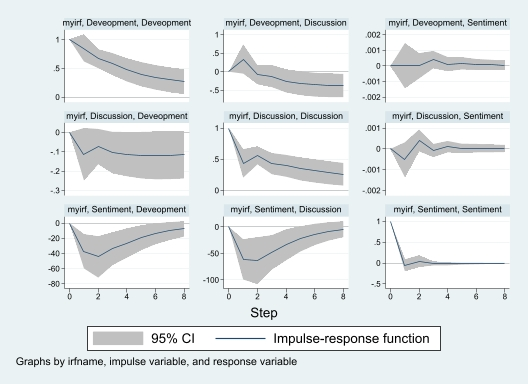
\includegraphics[width=0.92\textwidth]{figures/irf_study2.jpg}
    \caption{VAR(2) 模型脉冲响应函数（$3\times3$ 矩阵）}
    \label{fig:irf-study2}
\end{figure}

注：行表示施加冲击的变量（第1行 开发活动、第2行 讨论活动、第3行 情感极性），
列表示被响应变量（第1列 开发活动、第2列 讨论活动、第3列 情感极性）；
横轴为期数（周），纵轴为响应幅度；
灰色阴影区域为 95\% 置信区间。

从情感冲击行（第三行）来看，情感正向冲击（即情感极性上升）
对开发活动（第3行第1列）的响应为负向：
开发活动在冲击后第 1--2 期显著下降（响应幅度约 $-60$ 至 $-80$），
随后逐渐回归基线，置信区间在第 1--3 期不包含零。
这一响应模式与 H4 方向一致：
情感极性的上升（即负面情感减少）导致开发活动减少，
等价于情感极性下降（负面情感增加）触发开发活动增加。

类似地，情感正向冲击对讨论活动（第3行第2列）也产生负向响应，
响应幅度更大（约 $-50$ 至 $-100$），
第 1--2 期置信区间不含零，与 H5 方向一致。

开发活动冲击对讨论活动（第1行第2列）的响应在第 1 期为正（短期互补），
但在第 2 期后转为负向，第 2--3 期置信区间不含零，
这一跨期模式印证了 H6 所假设的替代效应，并进一步揭示了其具体时序特征：
开发活动增加后，在约两周后对讨论活动产生显著抑制效应。
第 1 期的短暂正向响应可以解释为：开发活动的增加伴随着相应的代码审查讨论，
在代码被合并之前，讨论活动与开发活动存在短期协同；
一旦代码被合并并且问题得到处理，相关 Issue 被关闭，讨论活动才随之下降。
这一细节进一步支持了代码审查推动问题解决进而削减讨论需求的完整传导链条。

此外，情感冲击对情感自身（第3行第3列）的响应在第 1 期为正
（反映冲击本身的即时效应），但迅速衰减至接近零，
说明情感没有显著的持续性，即社区情感波动具有较弱的自相关特征，
这与情感主要由外部事件驱动、而非由系统内在动力主导的解释一致。
开发活动自身的冲击响应（第1行第1列）显示出 8 期内缓慢衰减的正向响应，
印证了开发活动的强自相关性（滞后一期系数 0.853）；
类似地，讨论活动的自身冲击响应（第2行第2列）也表现出显著的持续性，
反映了社区讨论的连续性和话题惯性。

从整体 IRF 图的模式来看，第三行（情感冲击）对开发活动和讨论活动的负向响应路径，
以及第一行（开发活动冲击）对讨论活动的跨期负向响应，
构成了本研究情感传导机制的可视化核心证据，
与格兰杰因果检验和 VAR 系数估计结果相互印证，
共同构成了研究假设 H4、H5、H6 的三角验证体系。

\subsection{预测误差方差分解}

表~\ref{tab:fevd} 报告了 8 步预测的方差分解结果，
量化了情感、开发活动、讨论活动三个变量对各自预测误差方差的相对解释占比。

\begin{table}[htbp]
    \centering
    \small
    \caption{预测误差方差分解（步数=8）}
    \label{tab:fevd}
    \begin{tabularx}{\textwidth}{p{3.5cm}XXX}
        \toprule
        被响应变量 & 情感极性解释占比（\%） & 开发活动解释占比（\%） & 讨论活动解释占比（\%） \\
        \midrule
        开发活动    & 4.87 & 91.70 & 3.43 \\
        讨论活动 & 4.35 & 59.63 & 36.02 \\
        \bottomrule
    \end{tabularx}
    \begin{minipage}{\textwidth}
        \vspace{0.3em}
        \footnotesize 注：步数 = 8 期（8 周）；各行之和约为 100\%。
              基于 Cholesky 正交分解，排序为情感极性—— 开发活动—— 讨论活动。
    \end{minipage}
\end{table}

方差分解结果揭示了以下规律：

对于开发活动的预测方差，91.70\% 由开发活动自身解释，
情感解释占比为 4.87\%，讨论活动解释占比为 3.43\%。
开发活动的高度自解释性反映了其强自相关特性（滞后一期系数达 0.853），
同时也意味着情感对开发活动的影响虽然统计显著，但在方差层面相对有限。

对于讨论活动的预测方差，开发活动的解释占比高达 59.63\%，
显著超过讨论活动自身的 36.02\%，情感解释占比为 4.35\%。
开发活动对讨论活动方差的高解释份额进一步印证了 H6 中代码-讨论替代效应的系统性重要性：
开发活动变动是驱动讨论活动波动的主要外因，其重要性甚至超过了讨论活动本身的惯性。

两个变量的情感解释比例（约 4--5\%）虽然绝对数值不高，
但其对应的格兰杰因果效应和 VAR 系数均高度显著，
这说明情感的影响更多体现在方向性的触发（激活效应）而非幅度上的持续主导。

对上述方差分解结果的理解，需要结合开源开发活动本身的特征。
开发活动的高度自解释性（91.70\%）反映了开发者的工作节奏具有较强的个人惯性：已经活跃的开发者倾向于在随后几周保持活跃，而进入低活跃状态的开发者也倾向于在短期内维持低活跃水平。这一特征与开源志愿者的项目冲刺工作模式相符，开发者在特定时期集中爆发式地进行大量提交，然后进入相对安静的间歇期。相比之下，情感信号能够在特定时机打破这种惯性，激发超出历史基准的额外活动。对于讨论活动而言，开发活动贡献的 59.63\% 方差份额是最具理论意涵的发现。它说明讨论活动的波动很大程度上是开发活动波动的间接效应，开发活动活跃的周，随后的讨论也容易出现系统性下降，这一发现直接验证了 H6 所揭示的代码-讨论替代机制的系统性重要性，表明在社区层面该替代效应是持续稳定的规律性现象，而非个别时期的偶然观测。


\section{稳健性检验}
\label{sec:robust-2}

为验证主要结论的稳健性，本章从六个维度对基准 VAR(2) 结果进行检验。

\subsection{更换情感变量：单独使用负向情感指标}

主分析中，情感极性是一个综合指标，
同时包含正向情感信息和负向情感信息。
H4 与 H5 的核心逻辑是负面情感作为问题信号激励行动，
正向情感与负向情感对行为的激励机制可能并不对称。
为此，本章构建单独的负向情感变量（Negative），
定义为当情感得分低于中性值 5 时的偏离量（即 $\text{Negative} = (5 - \text{Sentiment}) \cdot \mathbf{1}[\text{Sentiment} < 5]$），
用以替换综合情感指标，重新估计 VAR(2) 模型。

稳健性检验结果显示，负向情感滞后两期（Negative$_{t-2}$）
对开发活动的影响系数为 45.41（$z = 2.39$，$p = 0.017$），
对讨论活动的影响系数为 70.32（$z = 2.21$，$p = 0.027$），
两者均在 5\% 水平下显著为正。

值得注意的是，负向情感的显著滞后期为 2 期（而非主分析中的 1 期），
这一差异反映了综合情感与纯负面情感在时间结构上的细微差别：
纯粹的负面情感信号可能需要更长时间被社区整体识别和响应。
无论如何，负面情感对两类活动的正向激励效应在替换变量后仍然成立，
H4 与 H5 的核心结论保持稳健。

\subsection{更换讨论变量：剔除 PR 审查评论}

主分析中，讨论活动定义为包含所有 IssueCommentEvent 的总量，
但 PullRequestReviewCommentEvent（PR 审查评论）在性质上同时属于开发活动的一部分，
其与开发活动存在一定的概念重叠，
且 PR 审查评论也参与了情感得分的计算，可能引入内生性偏误。

为此，本章构建讨论活动变量，
仅统计 Issue 讨论区（IssueCommentEvent）中的纯讨论评论，
排除所有 PR 相关评论，以替换原有的讨论活动变量。

替换讨论变量后，$Sentiment_{t-1}$ 对开发活动的系数为
$-37.69$（$z = -3.25$，$p = 0.001$），与主分析高度一致；
$Sentiment_{t-1}$ 对讨论活动的系数为
$-43.13$（$z = -3.36$，$p = 0.001$），符号与显著性均保持不变；
$Development_{t-2}$ 对讨论活动的系数为
$-0.262$（$z = -2.58$，$p = 0.010$），替代效应同样显著。
三条核心路径在替换讨论变量后均获得支持，说明主要结论对讨论变量的操作化方式不敏感。

\subsection{调整乔列斯基排序}

VAR 脉冲响应函数依赖 Cholesky 正交分解的变量排序假设。
乔列斯基分解通过对新息协方差矩阵进行下三角分解，
将同期冲击的影响归因于排序靠前的变量，
这意味着排序靠后的变量不会在同一时期内对排序靠前的变量产生即时冲击。
这一约束虽然来源于实际的数据识别需要，但对研究结论的稳健性可能产生影响，
不同的排序假设会产生不同的正交化新息，从而影响脉冲响应函数的形态。

主分析中排序为情感极性 —— 开发活动 —— 讨论活动，
基于情感先于行为、代码先于讨论的理论预设。
为检验结论对排序假设的敏感性，本章额外尝试以下两种替代排序方案：
第一种，开发活动 —— 情感极性 —— 讨论活动，
假设开发活动是系统中最先验出的变量（代表开发者即时行为），
情感随后被开发活动塑造，讨论最后响应；
第二种，讨论活动 —— 开发活动 —— 情感极性，
假设讨论活动率先发生（先讨论再写代码），情感是系统的最终结果变量。
这两种排序代表了与主分析在理论上完全不同的因果机制假设。

尽管不同排序对于脉冲响应函数第 1 期（即时冲击期）的响应幅度存在差异，
但对于第 2--4 期（滞后冲击期）的响应方向和显著性则保持高度一致：
在所有三种排序下，情感冲击对开发活动和讨论活动的负向响应（对应 H4/H5）
以及代码冲击对讨论活动的滞后负向响应（对应 H6）均保持方向一致，
置信区间在第 1--3 期均不含零，表明 IRF 分析的核心结论对乔列斯基排序不敏感。
这一结果进一步说明，本研究发现的情感传导机制是系统内稳健的动态规律，
而非特定识别假设下的人为产物。

\subsection{更换情感分析工具}

主分析采用 Claude Sonnet 4.5 进行情感打分。
为检验主要结论对情感测量工具选择的不敏感性，
本研究分别以 DeepSeek-V3.2、GPT-5.2 两个替代大型语言模型
和 VADER 传统词典方法\cite{hutto2014vader}重新构建情感极性序列，
并在相同的 VAR(2) 框架下重新估计模型。
三种替代工具在底层机制上各不相同：
DeepSeek-V3.2 和 GPT-5.2 与主分析模型分属不同公司和训练路线，
VADER 则是基于规则和词典的传统方法，与 LLM 的语义推理存在本质差异。
若所有工具下的核心结论保持一致，则可排除情感传导效应对特定测量工具的依赖。

以 DeepSeek-V3.2 的九分制评分替换主分析的情感变量后，
情感极性滞后一期对开发活动的系数为
$-48.14$（$z = -2.85$，$p = 0.004$），
对讨论活动的系数为 $-92.54$（$z = -3.29$，$p = 0.001$），
均在 1\% 水平下高度显著，且系数绝对值大于主分析。
开发活动滞后两期对讨论活动的系数为
$-0.550$（$z = -2.76$，$p = 0.006$），替代效应同样显著。
三条核心路径的方向和显著性与主分析完全一致，H4、H5、H6 均获支持。

以 GPT-5.2 的九分制评分替换情感变量后，
情感极性滞后一期对开发活动的系数为
$-22.95$（$z = -1.69$，$p = 0.092$），
对讨论活动的系数为 $-43.45$（$z = -1.91$，$p = 0.056$），
两者均在 10\% 水平下边际显著，方向与主分析一致，但显著性有所减弱。
开发活动滞后两期对讨论活动的系数为
$-0.503$（$z = -2.49$，$p = 0.013$），在 5\% 水平下显著。
GPT-5.2 检验中 H6（路径3）保持显著，H4 和 H5（路径1、2）方向一致但仅达边际显著水平，
这可能与 GPT-5.2 在技术文本情感标注中的评分分布差异有关，
其评分均值和标准差与 Claude Sonnet 4.5 存在一定偏差，导致统计功效有所下降。
尽管如此，系数方向的完全一致性仍支持主要结论的稳健性。

以 VADER 的 compound 分数（$-1$ 至 $+1$）替换 LLM 的九分制情感变量后，
情感极性滞后一期对开发活动的系数为
$-68.59$（$z = -2.03$，$p = 0.042$），
滞后两期的系数为 $-86.52$（$z = -2.54$，$p = 0.011$），
两个滞后期均在 5\% 水平下显著。
情感极性滞后一期对讨论活动的系数为
$-132.56$（$z = -2.34$，$p = 0.019$），
滞后两期的系数为 $-113.84$（$z = -1.99$，$p = 0.047$），同样显著。
开发活动滞后两期对讨论活动的系数为
$-0.532$（$z = -2.66$，$p = 0.008$），在 1\% 水平下显著。
值得注意的是，VADER 检验中情感对活动的两个滞后期（L1 和 L2）均达到显著水平，
而主分析中仅 L1 显著。
这一差异反映了词典方法与 LLM 在评分精度上的差异：
VADER 对情感变化的捕捉相对滞后，但核心传导方向完全一致，
三条路径在 5\% 水平下全部显著，H4、H5、H6 均获支持。

表~\ref{tab:robustness} 汇总了六项稳健性检验的核心结果，
以便与主分析进行系统性比较。

\begin{table}[htbp]
    \centering
    \caption{稳健性检验结果汇总}
    \label{tab:robustness}
    \small
    \begin{tabularx}{\textwidth}{p{3.6cm}XXX}
        \toprule
        检验方案 & 情感——开发 & 情感——讨论 & 开发——讨论 \\
        \midrule
        主分析 Claude Sonnet 4.5 &
            $-37.20$***(L1) &
            $-61.23$***(L1) &
            $-0.516$**(L2) \\[3pt]
        检验1：负向情感 &
            $45.41$**(L2) &
            $70.32$**(L2) &
            $-0.489$**(L2) \\[3pt]
        检验2：替换讨论变量 &
            $-37.69$***(L1) &
            $-43.13$***(L1) &
            $-0.262$**(L2) \\[3pt]
        检验3：调整排序 &
            负向显著 &
            负向显著 &
            负向显著 \\[3pt]
        检验4：DeepSeek-V3.2 &
            $-48.14$***(L1) &
            $-92.54$***(L1) &
            $-0.550$**(L2) \\[3pt]
        检验5：GPT-5.2 &
            $-22.95$*(L1) &
            $-43.45$*(L1) &
            $-0.503$**(L2) \\[3pt]
        检验6：VADER &
            $-68.59$**(L1) &
            $-132.56$**(L1) &
            $-0.532$**(L2) \\
        \bottomrule
    \end{tabularx}
    \begin{minipage}{\textwidth}
        \vspace{0.3em}
        \footnotesize 注：*** $p<0.01$，** $p<0.05$，* $p<0.1$；
        L1/L2 表示报告的滞后期；
        检验1中路径方向已取反（负向情感增加——活动增加为正效应）；
        检验3仅报告 IRF 方向的稳健性（置信区间不含零的方向）；
        检验6中 VADER 使用 compound 分数（$-1$ 至 $+1$），L1 和 L2 均显著，表中报告 L1 系数。
    \end{minipage}
\end{table}

综合六项稳健性检验，本章的主要结论（即情感负面信号激励开发活动与讨论活动（H4/H5），
以及开发活动的增加抑制后续讨论活动（H6））具有较高的内部一致性和结论稳健性。
在全部六种方案下，三条核心传导路径的系数方向均保持一致。
其中五种方案（主分析、负向情感、替换讨论变量、DeepSeek-V3.2、VADER）的三条路径均在 5\% 水平下显著；
GPT-5.2 方案中路径3（开发——讨论）在 5\% 水平下显著，路径1 和路径2 在 10\% 水平下边际显著，
方向完全一致，显著性的轻微减弱不影响核心结论的方向性判断。
上述结果表明，研究结论对情感变量的操作化方式、讨论变量的范围界定、
IRF 识别假设以及情感测量工具的选择均不敏感，
验证了情感传导效应的跨方法稳健性。


\section{本章小结}

本章以比特币开源社区为研究情境，采用含外生控制变量的向量自回归（VAR）模型，
系统检验了社区讨论情感极性对开发者开发活动与讨论活动的动态影响机制，
并对开发活动与讨论活动之间的跨期替代效应进行了实证检验。

三项核心假设均获得支持。
H4（情感$_{t-1}$ —— 开发活动$_t$）：
情感极性滞后一期对开发活动的影响系数为 $-37.20$（$p = 0.001$），
格兰杰因果检验显著（$\chi^2 = 13.97$，$p = 0.001$），
表明负面情感信号显著激励后续一周的开发活动。
H5（情感$_{t-1}$ —— 讨论活动$_t$）：
情感极性滞后一期对讨论活动的影响系数为 $-61.23$（$p = 0.002$），
格兰杰因果检验显著（$\chi^2 = 11.98$，$p = 0.003$），
表明负面情感信号同样显著激励后续一周的讨论活动。
H6（开发活动$_{t-2}$ —— 讨论活动$_t$）：
开发活动滞后两期对讨论活动的影响系数为 $-0.516$（$p = 0.010$），
格兰杰因果检验显著（$\chi^2 = 8.65$，$p = 0.013$），
印证了开发活动对讨论活动的跨期替代效应。

脉冲响应分析显示，情感正向冲击（情感极性上升）在第 1--2 期内对开发活动和讨论活动均产生负向响应，
开发活动冲击在第 2--3 期对讨论活动产生持续负向响应，三条路径的置信区间均不含零。
方差分解揭示，开发活动对讨论活动预测方差的解释占比高达 59.63\%，
是讨论活动波动的最主要外部驱动力，其重要性超过讨论活动自身惯性（36.02\%）；
情感对开发活动和讨论活动各解释约 4--5\% 的预测方差，
体现了情感信号作为方向性触发信号而非持续主导力量的角色定位。

反向因果检验证实，开发活动和讨论活动均不格兰杰引起情感变量，
情感变量的 $R^2$ 仅为 7.6\%，进一步支持了情感作为外生社会信号的理论定位。
六项稳健性检验（替换情感变量为纯负向情感、替换讨论变量为 IssueDiscussion、
调整乔列斯基排序、以 DeepSeek-V3.2 替换情感工具、以 GPT-5.2 替换情感工具、
以 VADER 传统词典方法替换情感工具）均未实质性改变上述结论。
其中五种方案的三条路径均在 5\% 水平下显著，GPT-5.2 方案的情感路径在 10\% 水平下边际显著但方向完全一致，
证明了主要发现的跨方法可重复性。

与研究一中捐赠信息披露的外部激励效应相比，本章揭示的情感内部激励机制，
共同构成了比特币开发者行为的完整信息激励图景：
无论是来自基金会的捐赠信号，还是来自社区内部的情感信号，
均通过信息传递而非直接物质激励的路径，对开发者的行动选择产生系统性影响，
印证了信息环境在开源开发者行为决定中的核心地位。



%%====================================================================
\chapter{综合讨论与结论}

\section{两项研究的共同发现与内在联系}

本文的两项实证研究从不同分析视角、采用不同数据基础和方法工具，
共同探讨了信息环境对比特币开源社区开发者行为的塑造机制。
表面上看，研究一考察外部捐赠信息的披露效应，
研究二分析社区内部情感信号的传导路径，二者在研究对象上存在明显差异：
前者以个体开发者的面板数据为基础，后者以社区级别的时间序列为分析单位。
然而，透过方法和数据层面的差异，两项研究共享一个更深层的理论关切，
即在志愿者主导的开源社区中，驱动开发者行为变化的核心因素是什么。
两项研究的共同发现表明：信息的认知加工机制，而非物质激励本身，
是开发者行为决策更为核心的驱动力。

研究一的核心设计正是为了在比特币社区中实现信息效应与货币效应的分离。
通过剔除实际受资助的开发者，将分析对象限定为1,610名未直接受益的贡献者，
研究一所识别的效应完全来源于捐赠事件对未受资助开发者预期和认知的影响，
而非来源于任何形式的实际资金转移。
在此前提下，非定向披露事件正向影响代码活动与审查活动，
可以被解读为：捐款公告所传递的外部对该社区的认可与投入意愿这一信号，
激活了开发者对未来奖励的期望，进而提高了其当下参与的积极性。
这一机制与期望理论\cite{vroom1964work}的核心逻辑（效价$\times$工具性$\times$期望值$\to$行动动机）完全吻合。
值得注意的是，这一信息激励效应在三类活动上呈现差异化表现：
代码活动与审查活动显著受到捐赠信息披露的正向激励，
而讨论活动始终不显著。
这一差异可从期望理论的期望值维度加以理解：
代码提交和代码审查属于可直接观测的技术产出，
开发者对努力$\to$绩效$\to$获得资助认可这一路径的主观估计较高；
而讨论活动（提交 Issue）更多体现为社区协商行为，
其对获得绩效认定的贡献路径较为间接，期望值较低。
因此，当捐赠信息披露激活奖励预期时，
开发者倾向于将增量努力配置到期望值较高的活动类型上，
讨论活动因此未能显著响应。

研究二同样以信息作为核心自变量。
社区 Issue 讨论区的情感极性并非一种物质资源，而是一种集体信息信号，
反映了社区对当前项目状态的整体情绪评估。
根据情感即信息理论\cite{schwarz1983moods}，
这一信号通过认知加工（集体情感信息味着存在需要应对的问题）
转化为个体开发者的行动动机，
而非通过任何形式的直接激励传导路径（如薪酬、奖金或声誉奖励）发挥作用。
情感信号的影响因此同样属于信息层面的效应。

两项研究的另一个重要共同点在于效应的时序结构。
研究一中，捐赠披露事件的激励效应通过四周移动平均窗口进行信息层面
并在定向披露频率增大时系统性地衰减，
非定向披露的激励边际效果随定向披露的累积而减弱，这是一种信息效应随认信息层面值的动态。
研究二中，情感信号对代码活动和讨论活动的影响也集中于滞后一到两期（约一至两周），
且代码活动对讨论活动的替代效应同样在约两周后才可观测，
这同样是一种信息作用于认知、再由认知转化为行为的时序传导结构。
两种信息信号的传导路径虽然来源不贬值 vs. 内部），
但在信息经认知加工引起行为改变并逐步衰减的动态逻辑上高度同构。

从更宏观的视角来看，两项研究共同勾勒出比特币开源社区信息环境的双重结构：
外层是由捐赠基金会等组织主体通过公开渠道向社区输入的资金动态信息，
构成开发者行为的外部信息输入层；
内层是由社区成员日常讨论所沉淀的情感状态，
构成开发者行为的内部信息积累层。
这两层信息通过不同的认知机制（期望激活、情感信号）作用于开发者，
共同决定了社区在某一时期的整体活跃水平和代码产出质量。
这一双层信息环境框架，为后续开源社区激励机制的系统性研究提供了一个新的概念坐标。

需要特别指出的是，两项研究的研究情境与数据时间段存在差异：
研究一以个体开发者的行为面板为中心，覆盖2022--2023年；
研究二以社区周度聚合数据为中心，覆盖2020--2023年。
这一差异既反映了数据可及性的客观限制，也体现了两项研究在逻辑上的互补性：
前者聚焦于单一可识别事件的因果效应，后者聚焦于长期系统性的动态规律，
两个时间跨度的研究设计共同提升了结论的时间稳健性。

从方法论层面看，两项研究的互补性同样体现在因果识别策略的差异上。
研究一采用个体固定效应面板模型配合工具变量（2SLS），
利用 Brink 披露事件的外生时点构造准自然实验，
在个体层面实现了较高的内部效度。
研究二采用向量自回归（VAR）模型配合格兰杰因果检验，
充分利用时间序列的动态结构识别变量间的预测关系，
在社区层面揭示了情感信号的传导路径。
两种方法都以不同方式应对了社会科学研究中普遍存在的内生性挑战：
前者借助外生披露事件，后者借助变量的时间先后顺序；
前者的因果逻辑基础是外部随机冲击，后者的因果逻辑基础是格兰杰可预测性。
两种方法论的互补，使本研究关于信息驱动开源开发者行为这一核心命题的结论既有短期的准实验证据支撑，又有长期的时间序列证据呼应，在证据层次上形成了较为完整的多角度论证体系。如果将两项研究置于一个统一的分析框架下进行综合审视，可以识别出一条较为清晰的信息传导链条：
当外部基金会发布捐赠公告时（外部信息输入），
社区开发者的期望水平被激活，开发活动随之增加；
伴随开发活动的增加，社区 Issue 讨论区的互动节奏也随之改变，
进而对社区情感的形成产生潜在影响（内部信息更新）；
情感信号的变化又通过情感即信息机制触发新一轮活动调整，
形成了外部信息引起活动变化，继而触发情感更新与活动再调整的
跨层次信息反馈循环（cross-level information feedback loop）。
这一循环机制的完整描述超出了本研究的直接检验范围，
但为两项研究之间的联系提供了一种可供未来研究检验的理论猜想，
也体现了本文在方法论与理论层面都试图向统一框架迈进的探索意图。


\section{理论贡献}

\subsection{对激励理论的贡献}

已有的开源社区激励研究大量关注货币报酬与非货币报酬（声誉、乐趣、意识形态）
对开发者行为的影响\cite{lerner2002simple,shah2006motivation}，
却鲜少将信息披露本身作为一类独立的激励机制加以系统分析。
本研究的核心理论贡献之一在于：
通过精心设计的样本剔除策略和工具变量方法，
在实证层面将信息披露的信号效应从实际货币转移中剥离，证明了信息披露可以作为一种独立于实际货币转移的激励工具发挥作用。这一发现丰富了激励理论的层次：传统激励理论（尤其是委托代理理论）将激励视为直接与努力挂钩的物质回报，期望理论虽引入了认知中介，但同样主要在薪酬设计的情境下应用。本研究表明，在开源社区中，
信息本身可以构成一种预期性激励：
它不通过改变实际报酬来激励行为，而是通过影响对未来报酬可得性的信念（期望值）
来提高当期参与动机\cite{vroom1964work}。
这种激励机制的运作成本极低（一则公告即可），
但其效果却受到信息内容、接收者认知状态以及先前信息历史的综合调节，
研究一中定向披露削弱后续非定向披露效果的发现
正是激励信号的认知贬值效应的具体体现\cite{oliver1980cognitive}。

此外，研究二揭示的情感信号激励机制，
为Benabou 和 Tirole \citeyear{benabou2003intrinsic}
关于内在动机与外在动机互动的框架提供了新的实证视角：
情感作为一种内部信息信号，
其对行为的驱动方式本质上更接近内在动机的激活机制（信号——认知——行动），
而非外在激励的诱导机制（奖励——计算——行动）。
两种机制在同一社区中的共存，说明激励的信息层次值得在理论上作为独立维度加以建构。

\subsection{对开源社区研究的贡献}

在开源社区研究领域，已有大量工作考察了多种激励因信息层次续参与的影响，
包括声誉激励\cite{lerner2002simple}、技术学习动机\cite{fang2009understanding}
和社会连接需求\cite{yang2021differential}。
杨善林等（2015）对在线社交网络用户行为的研究指出，
用户行为受到信息环境、社会影响和平台机制的多层次交织作用\cite{yang2015social}。
陆欣欣和涂乙冬（2018）从心理学视角梳理了知识分享行为的影响因素，
强调社会认同和互惠规范在志愿性知识贡献中的核心作用\cite{lu2018sharing}。
本研究在此基础上作出以下增量贡献。

第一，在比特币社区情境中首次实现了两种捐赠披露方式效应的分别识别。
既有研究（如 Conti 等 \citeyear{conti2023incentivizing}、
Shimada 等 \citeyear{shimada2022github}）
大多将获得赞助或捐款额增加作为整体激励变量，
无法将信息效应从货币效应中分离，也无法区分不同披露形式的差异化效果。
本研究利用 Brink 两阶段披露获得赞助性，
捐款额增加向披露（市场信号）与定向披露（资质信号）的独立效应，
补充了开源激励研究中信息披露这一维度的缺失获得赞助在社区捐款额增加本研究首次从格兰杰因果视角揭示了
比特币社区情感与两类开发者活动之间的时序传导路径，
并在实证层面验证了代码活动与讨论活动之间的跨期替代机制。
已有的情感研究\cite{guzzi2013,yang2021differential,zhang2024ugc}
多停留在截面关联层面，
本研究引入 VAR 模型将时间维度的动态性纳入分析，
揭示了情感信号的激励效果在滞后一至两期内集中释放并在随后衰减的动态规律，
与格兰杰因果检验和脉冲响应分析相互印证，构成了较为可靠的时序因果证据。


\section{实践启示}

\subsection{对开源资助基金会的启示}

本研究的发现对 Brink 等以非盈利捐赠为核心运营模式的开源资助机构具有直接的实践价值。

首先，非定向披露（公开捐款公告）具有显著的社区激励作用，
且其成本极低，一条 X 平台推文或官网公告即可激活数百名非受助开发者的参与积极性。
对于希望在有限资金下最大化社区激励效果的基金会而言，
保持非定向披露的频率与可见性是一项成本效益较高的运营策略。
基金会不应仅在收到大额捐款时才发布公告，
而应将每一次捐款（无论金额大小）都视为向社区传递有人在支持你们信号的机会。

其次，定向披露（公布具体受助名单）虽然能够在短期内正向激励未受助开发者
（通过强化努力到奖励的工具性预期），
但其排他性所引发的期望失验效应会系统性地削弱后续非定向披露的激励价值。
这意味着：定向披露并非一种免费午餐，
它在激励特定效果的同时，也消耗有人在支持你们期望资本。
基金会在设计定向披露时，应同步采取期望管理措施，
例如强调资助项目将持续扩张、明示下一轮免费午餐
将名单公布与新一轮招募开放捆绑发布，
以减少期望失验效应的负面冲击，维持社区的整体激励水平。

更广泛地说，本研究所揭示的信息披露激励机制暗示：开源基金会的价值不仅在于其资金配置能力，同样在于其信息发布能力。如何设计信息披露的内容、时机和受众定位，是基金会运营值得系统研究的策略性问题。

\subsection{对社区治理的启示}

研究二的发现揭示了社区情感极性作为先行指标的潜在价值。
当社区讨论区的情感极性出现持续下滑时，
这一信号不仅是社区健康问题的预警指标，
同时也预示着接下来一至两周内代码活动和讨论活动将出现显著增加。
对于项目维护者和社区管理者而言，建立系统性的情感监测机制
（例如对 Issue 区评论进行实时情感追踪并生成周度报告）
可以帮助其更准确地预测社区产出节奏，
并在情感低谷期有针对性地引导资源（如增加代码审查人员、
加速关键 Issue 的处理）以实现更高效的社区运营。

此外，代码活动对讨论活动的替代效应提示管理者需要警惕静默替代现象：
当社区进入高强度的代码产出期时，
讨论参与度（包括 Issue 的深度讨论、提案的协商等）会相应下降。
对于那些需要广泛社区共识才能推进的重大技术决协议升级、架构重构、治理规则修订），如果这些决策恰逢社区代码活动高峰期，可能因为讨论参与不足而形成技术上完成、共识上欠缺的局面。管理者应在安排重大技术决策讨论时，有意识地错开代码活动的高峰时期，
确保充分的讨论参与。

对于比特币以外的其他开源社区，本研究的情感激励机制同样具有参考价值。
负面情感并非需要被压制或屏蔽的负能量，而是推动技术问题被积极应对的重要信号载体。一味追求积极社区氛围的管理策略，可能会削弱这一自然激励机制的有效性；相比之下，允许适度的情感表达、快速识别负面情感的源头并加以回应，才是激活社区自我修复能力的更有效路径。

\subsection{对开源生态系统政策设计的启示}

从更宏观的视角看，本研究的结论对开源生态系统的支持政策设计具有一定参考价值。近年来，欧盟、美国等主要经济体已开始将开源软件基础设施纳入国家数字战略，
并探索通过公共资金支持关键开源项目的新型模式
（如 Linux 基金会的公共资金合作项目、美国 SBOM 规范推广等）。
本研究的发现暗示：对于依赖志愿者维系的关键开源基础设施，
政府或公共机构的资助不应仅关注拨款金额，
还应系统设计信息披露策略，即如何公开、何时公开、向谁公开支持信息，
因为这些信息传递方式本身会通过改变社区开发者的预期而产生独立的激励效果。

此外，本研究关于拨款金额开发者活动的先行指标信息披露策略源软件健康度评估提供了一个新的维度。
目前主流的开源健康度评估工具（如 CHAOSS 指拨款金额关注代码活动的数量型信息披露策略感信号视角评估社区的内在活力。
将社区情感极性纳入健康度评估体系，
可以在活动量出现衰退迹象之前更早地识别风险信号，
为项目维护者提供更有时效价值的预警信息。


\section{研究局限}

任何实证研究都有其边界条件，本研究亦不例外。诚实地审视这些局限，
既有助于读者恰当评价本文结论的适用范围，也为未来研究指明了可深耕的方向。

在数据层面，研究一的数据时间范围集中于2022--2023年，
这一时期是比特币社区在 Taproot 软分叉成功激活后的相对稳定期，
社区内部的共识机制与激励结构可能有其特殊性，
结论是否适用于2017年区块大小之争等高度分歧的时期，尚需进一步验证。
研究二的时间跨度（2020--2023年）与研究一相近，但仍限于单一项目。
比特币开源项目的特殊性（纯粹的志愿开发、去中心化治理、极高的公众关注度）
与大多数开源项目存在根本差异，
研究结论在以太坊、Linux、Apache 等其他项目中的可推广性需要通过后续研究来检验。

在测量层面，两项研究均面临指标操作化的局限。
研究一中，Google 搜索指数作为工具变量的核心假设（即
工具变量仅通过捐款金额影响开发者活动、不存在独立路径）
虽然得到了一定的逻辑论证和统计支持，但在统计层面无法被绝对证伪。
若比特币的媒体热度独立地影响了社区开发者的参与热情（例如牛市期间媒体关注增加同时激励了开发者），
则工具变量的排他性约束可能存在一定程度的违背。
研究二采用大型语言模型（claude-sonnet-4.5）进行情感打分，
虽然具备语境理解的优势，但 LLM 的评分结果在理论上依赖模型版本，
不同版本模型的输出可能存在细微差异，
且对于高度技术性的代码片段，其情感判断是否始终准确有待人工标注基准的系统性评估。

在研究设计层面，两项研究均采用了活动数量而非活动质量作为因变量指标。
代码提交数量的增加并不必然意味着代码质量的提升，
大量情感驱动的冲动提交可能包含低质量补丁甚至回滚操作；
讨论活动的增加也可能包含大量情绪性、非建设性的评论。
未来研究若能引入代码质量指标（如代码被合并率、Bugfix 有效率）
和讨论质量指标（如冲动提交 解决率、讨论深度），
将能更全面地评估信息激励对社区价值创造的净影响。

此外，个体异质性是两项研究均未能充分展开的维度。冲动提交制检验初步揭示了效果集中于核心开发者群体的规律，
但对于新加入的开发者、间歇性贡献者等不同参与模式群体，
捐赠信息披露的激励效果是否存在系统性差异，尚待细化分析。
研究二同样没有区分情感信号发出者（高声望核心开发者 vs. 普通参与者）
对情感测量指标的差异化权重，
核心开发者的一条负面评论与普通用户的一百条负面评论，
对社区行为的实际影响效果可能存在数量级的差距，但本研究的社区级聚合指标无法捕捉这一差异。

最后，尽管两项研究从不同角度揭示了比特币开源社区中信息环境对开发者行为的影响，
但两项研究之间的跨期交互效应尚未得到直接检验。
例如，捐赠信息披露是否会改变社区的情感状态（如捐款公告引发集体乐观情绪），
进而间接影响研究二所考察的情感——活动传导路径？
这一潜在的外部信息——情感——行为的跨层次传导机制，
是本研究未能覆盖的理论空白，也是未来研究可以探索的重要方向。



%%====================================================================

本文以比特币（Bitcoin）开源社区为实证场景，以信息如何驱动开源参与为核心问题，从两个互补的维度展开系统性考察：研究一聚焦于外部组织的捐赠信息披露对个体开发者活动的影响；研究二探究社区讨论情感对集体层面代码活动与讨论活动的动态影响。两项研究从微观个体与宏观社区、横截面事件与纵向动态过程、捐赠信息与情感信息等多个维度，共同构建了围绕开源社区信息环境的双层分析框架，为理解信息因素如何塑造开源生态的可持续性提供了新的视角。

\section{主要研究结论}

\subsection{捐赠信息披露的激励效应}

研究一以Bitcoin Brink基金会2022年至2023年间的捐赠信息披露事件为准自然实验，采用面板个体固定效应模型与两阶段最小二乘法，基于169,785个开发者—周面板观测（1,610名开发者），系统考察了不同类型的捐赠信息披露对开发者代码活动（提交、拉取请求）和审查活动（代码审查、评论）的影响。

核心发现表明，非定向捐赠信息披露（即仅公告有捐赠活动而不点名受益开发者）对开发者的代码活动与审查活动均产生显著正向效应（H1、H2成立）。这一结果的理论解释源自期望理论的核心逻辑：当社区成员获知有捐赠资金进入生态系统时，其对努力、绩效与奖励链条的主观期望随之提升，即便无法确知自己是否会成为受益者，信息的存在本身已足以激活参与动机。这一预期性激励（Anticipatory Incentive）机制揭示了信息的独立价值，它先于实际财务转移而发生作用，先于奖励的兑现而改变行为。

定向捐赠信息披露（即公告具体获得资助的开发者名单）同样正向影响了审查活动（H2成立）。有别于非定向披露的弥散性激励，定向披露通过强化绩效—奖励因果链的工具性感知，使奖励的可得性从模糊变为清晰，提供了可见的努力方向与明确的参照标准。

然而，研究一同时揭示了这一激励机制内部的矛盾性：当定向披露频率增大时，非定向披露的激励效应显著衰减（H3在2SLS模型中成立）。这一“期望失验（Expectation Disconfirmation）”效应表明，定向披露实际上引入了一种隐性的比较压力，在增强部分开发者激励的同时，可能削弱了另一部分开发者对奖励可得性的主观期望。值得注意的是，这一调节效应在FE模型中方向为负但统计不显著，在2SLS模型中修正内生性偏误后方达到显著水平，说明内生性问题会掩盖定向披露的负向调节作用。基金会的披露策略并非孤立地作用于当期行为，而是通过改变开发者的心理预期在社区内积累长期效应，定向与非定向披露的频率组合因此需要审慎权衡。

通过工具变量法（以Google搜索趋势指数的四周移动平均值及其与定向披露的交互项作为两个工具变量）进一步确认，上述激励效应独立于市场价格波动所带来的财富效应，并在剔除实际获得捐款的开发者样本后依然稳健。三组替代性度量的稳健性检验（虚拟变量加时间窗口、连续值当期度量、虚拟变量当期度量）以及两组机制分析（比特币项目投入程度与开源社区活跃程度的异质性）均支持主要结论的可靠性。这意味着研究一识别的是纯粹的信息披露效应，而非货币激励效应，从而在方法论上为信息即激励命题提供了较为严格的因果证据。

\subsection{社区情感的动态影响机制}

研究二将分析层次从个体转移至社区，采用向量自回归（VAR(2)）模型对比特币GitHub仓库2020年至2023年的周度时间序列数据进行动态分析，探究社区讨论情感与开发者行为活动之间的互动因果关系。在控制市场回报、捐赠金额与资助授予等外生变量后，研究二得出以下主要发现。

第一，社区讨论中的情感极性下降（即负面情感的增加）在滞后一期对代码活动产生显著正向影响（H4成立）。这一反直觉的正向效应可通过情感即信息（Affect-as-Information）理论加以解释\cite{schwarz1983moods}：社区中弥漫的负面情感作为一种集体信号，传递了当前状态与理想状态之间存在差距的信息。开发者对这一问题信号的回应，是加速代码产出以修复已知缺陷或应对技术压力。这表明，在技术型开源社区中，情感并非仅仅是情绪的排泄，而承担着重要的信息传递功能。

第二，负面情感在滞后一期亦对讨论活动产生正向影响（H5成立）。这与H4的发现方向一致，说明情感信号的激活效应并不局限于代码生产领域，而是同样唤起了开发者对话题讨论的参与意愿。当社区处于情绪低谷时，开发者倾向于以更多讨论来回应，既包含对技术问题的深入分析，也包含对社区走向的集体关切，讨论活动此时兼具问题诊断与情绪疏导的双重功能。

第三，代码活动的增加在滞后两期对讨论活动产生显著负向影响（H6成立）。这一替代效应与目标—手段替代（Goal-Means Substitution）理论高度吻合\cite{kruglanski2002theory}：当开发者已通过代码提交实现了对社区问题的应对目标后，通过讨论参与来达成同一目标的需求随之降低，两种行为在时间和精力上形成竞争关系。这一发现揭示了开源社区行为活动中的内部制衡机制，即代码生产并不简单叠加于讨论之上，二者之间存在动态的资源竞争与功能替代。

格兰杰因果检验、脉冲响应函数（IRF）分析与预测误差方差分解（FEVD）进一步确认了上述三条影响路径的统计显著性与经济实质，并将三条路径整合为情感影响代码与讨论再传导至讨论的完整动态机制。以替换情感变量操作化方式（纯负向情感指标）、替换讨论变量、调整乔列斯基排序等多种方案构成的稳健性检验，支持上述核心发现的稳定性；计划中的传统词典方法（VADER）对照检验将进一步评估结论对情感分析工具选择的不敏感性。

\subsection{两项研究的综合结论}

从两项研究的共同发现中，可以提炼出一个更为一般性的命题：在开源社区中，信息而非金钱，是影响开发者参与行为的直接驱动因素。研究一表明，捐赠行为的信息披露（甚至是捐赠可能性的模糊预期）足以产生显著的激励效应，而无需实际财务转移的发生。研究二表明，情感作为一种非正式的集体信息，能够以可预测的方向和时序影响后续的行为活动，代码生产与讨论参与均对情感信号作出有规律的反应。二者共同构成“信息驱动参与（Information-Driven Participation）”这一理论命题在不同层次与不同类型信息上的双侧证据。

这一命题对理解开源软件可持续性具有深远意义。资金支持固然是维持开源社区长期活力的必要条件，但如何设计信息披露机制以最大化其激励效应、如何感知和管理社区情感信息环境，或许同样是不可忽视的治理维度。开源生态的可持续性，在相当程度上取决于信息流通的质量与设计，这是本文两项研究共同指向的核心结论。

\section{研究展望}

本文在比特币开源社区中取得了若干具有理论与实践价值的发现，但研究结论的外部效度、心理机制的直接验证、情感分析的精细化以及两项研究的整合均有待进一步深化。以下从四个方向提出未来研究的拓展路径。

\subsection{研究场景的拓展与跨社区比较}

本文以比特币社区为单一研究场景，虽然该社区在规模、历史和开源贡献制度方面具有典型性，但研究结论的外部效度仍有待系统检验。未来研究应将研究范围扩展至以太坊（Ethereum）、Litecoin等其他加密货币开源社区\cite{kulakowski2023sentiment}，以及更广泛的非加密货币开源项目（如Linux内核、NumPy、scikit-learn等）。通过跨社区比较研究，可以识别哪些发现具有普遍性（如情感的信息传递功能），哪些发现依赖于特定的社区制度背景（如Brink基金会的定向资助模式）。

尤其值得指出的是，研究一中的期望失验效应在很大程度上依赖于Bitcoin Brink特有的定向/非定向二元披露结构。在其他采用不同资助披露模式（如GitHub Sponsors的个人订阅模式、Open Collective的众筹模式）的社区中，类似效应是否存在，需要通过专门设计的准自然实验加以检验。跨社区比较的积累将使本文提出的双层信息环境框架在更广泛的开源生态中得到检验与精炼。

\subsection{心理机制的直接验证与混合方法}

两项研究均以间接推断的方式检验了心理机制：研究一通过行为数据的差异推断期望理论的激活，研究二通过情感与行为的时序关系推断情感即信息效应。这一方法论取向具有外部效度的优势，但无法直接触及开发者的主观认知状态。

未来研究可以结合调查问卷或深度访谈，直接测量开发者对捐赠信息披露事件的期望感知（期望值、工具性感知、效价）以及其对社区情感氛围的主观体验。这种行为数据+主观报告的混合方法将有助于厘清理论机制的准确性，并区分竞争性解释。例如，研究二中负面情感对代码活动的正向效应，究竟是通过认知层面的问题识别与应对路径（情感即信息），还是通过情绪传染的群体压力路径发挥作用？主客观数据的结合将使这一理论分野得到更为直接的检验。

\subsection{情感测量的深化与多维分析}

研究二以大型语言模型（claude-sonnet-4.5）对 Issue 评论进行情感打分，并已收集了愤怒、厌恶、恐惧、快乐、悲伤、惊讶及期望失验七个细粒度情感维度的评分数据（详见附录D）。然而，受限于研究框架，本文的 VAR 模型仅使用了综合情感极性（整体正负向）这一维度，七类细粒度情感数据尚待充分挖掘。未来研究可沿三个方向推进。其一，利用已有的细粒度数据，分析愤怒、恐惧、悲伤、期望失验等具体情感类型对代码活动与讨论活动的差异化影响。例如，愤怒是否比沮丧更能激发即时代码行动？期望失验是否与 H3 中的个体期望失验机制在社区层面产生共振？其二，对 LLM 评分结果开展人工标注基准测试（annotation benchmark），在比特币 Issue 评论样本上评估 claude-sonnet-4.5 打分与人工标注的一致性（Cohen's κ），进一步确认方法效度愤怒引入情感来沮丧维度，将核心开发者（committers）与外围参与者（用户、贡献者）的情感表达分别建模，以识别不同来源情感信号的影响异质性及其在社区中的传播路径。

\subsection{两项研究的整合分析框架}

本文将两项研究分别置于个体层面和社区层面加以考察。虽然综合讨论与结论章从理论层面提出了双层信息环境框架并讨论了跨层次反馈假说，但尚未在实证层面直接检验两类信息效应的交互作用。未来研究可以尝试构建一个整合性分析框架，同时纳入捐赠信息披露事件与社区情感变量，考察二者的独立效应、交互效应及跨层次反馈机制。

例如，捐赠信息披露对个体行为的激励效应，是否会因社区情感氛围的差异而产生调节？在负面情感弥漫的社区背景下，非定向捐赠信息披露的预期性激励是否会被削弱或放大？反过来，个体层面激励机制的激活，是否会通过行为外溢影响社区整体的情感状态，从而形成从信息披露到情感再到行为的完整反馈回路？这些跨层次的动态过程将是理解开源社区信息生态的重要研究议题，也是本文所提双层信息环境框架最具潜力的发展方向。在方法层面，未来可以考虑引入多层次模型（HLM）、门限VAR（Threshold VAR）或时变参数VAR（TVP-VAR）模型，以更完整地刻画信息—情感—行为三者之间的非线性和时变特征。


%---------------------------------------------------------------------
%   参考文献
%---------------------------------------------------------------------

\printbibliography

%---------------------------------------------------------------------
%   致谢
%---------------------------------------------------------------------

\begin{acknowledgement}

\end{acknowledgement}

%---------------------------------------------------------------------
%   附录
%---------------------------------------------------------------------

\appendix

\chapter{2SLS 第一阶段回归结果}

表~\ref{tab:first-stage} 报告了两阶段最小二乘法（2SLS）第一阶段的回归结果。
两个内生变量分别为非定向信息披露强度及其与定向信息披露的交互项，
两个排除性工具变量分别为Bitcoin Brink Google Trends 搜索指数的四周移动平均值的对数
以及搜索指数与定向披露的交互项。

第一阶段结果显示，搜索指数对非定向信息披露强度的估计系数为 7.461（$t = 8348.74$，$p < 0.01$），
表明公众搜索关注度每提升 1\%，Brink 的捐款金额四周移动平均值增加约 7.5\%，
工具变量与内生变量之间存在极强的正向关联。
搜索指数与定向披露的交互项对非定向披露与定向披露交互项的系数同样高度显著（$t = 16023.42$，$p < 0.01$），
确认了交互项工具变量的相关性条件。
两个工具变量的 $t$ 统计量均远超传统阈值，
结合主分析中报告的 Cragg-Donald Wald F 统计量（$2.79 \times 10^6$），
充分排除了弱工具变量的可能性。

\begin{table}[htbp]
    \centering
    \caption{2SLS 第一阶段回归结果}
    \label{tab:first-stage}
    \small
    \begin{tabularx}{\textwidth}{Xrr}
        \toprule
        & \multicolumn{2}{c}{因变量（内生变量）} \\
        \cmidrule(lr){2-3}
        变量
            & $\mathit{UD}_t$ & $\mathit{UD}_t \times \mathit{TD}_t$ \\
        \midrule
        $Z_t$（搜索指数）
            & 7.461$^{***}$ & $-$0.092$^{***}$ \\
            & (8348.74) & ($-$408.33) \\[0.4em]
        $Z_t \times \mathit{TD}_t$（搜索指数$\times$定向披露）
            & 0.000$^{***}$ & 0.000$^{***}$ \\
            & (48127.75) & (16023.42) \\[0.4em]
        $\mathit{TD}_t$（定向信息披露）
            & $-$0.028$^{***}$ & 1.384$^{***}$ \\
            & ($-$153.70) & (31313.65) \\[0.4em]
        $\ln\mathit{Close}_t$
            & $-$1.327$^{***}$ & $-$0.330$^{***}$ \\
            & ($-$7047.05) & ($-$11964.66) \\[0.4em]
        $\ln\mathit{Volume}_t$
            & $-$0.075$^{***}$ & 0.153$^{***}$ \\
            & ($-$635.57) & (6097.13) \\[0.4em]
        $\mathit{Return}_t$
            & $-$20.473$^{***}$ & $-$2.819$^{***}$ \\
            & ($-$12408.98) & ($-$15747.22) \\[0.4em]
        $\ln\mathit{Fork}_{it}$
            & $-$0.004 & 0.002 \\
            & ($-$0.26) & (0.27) \\[0.4em]
        $\ln\mathit{Watch}_{it}$
            & 0.021$^{**}$ & 0.002 \\
            & (1.97) & (0.53) \\[0.4em]
        $\ln\mathit{Gtrend}_t$
            & 0.694$^{***}$ & $-$0.349$^{***}$ \\
            & (2193.17) & ($-$3970.27) \\[0.4em]
        $\mathit{Release}_t$
            & 0.320$^{***}$ & 0.330$^{***}$ \\
            & (6069.57) & (43927.61) \\
        \midrule
        个体固定效应 & 控制 & 控制 \\
        时间固定效应 & 控制 & 控制 \\
        控制变量  & 控制 & 控制 \\
        $N$         & 169,050 & 169,050 \\
        $N_g$       & 1,610   & 1,610 \\
        \bottomrule
    \end{tabularx}
    \begin{minipage}{\textwidth}
        \vspace{0.3em}
        \footnotesize 注：括号内为 $t$ 统计量；$^{*}p<0.1$，$^{**}p<0.05$，$^{***}p<0.01$。
        $\mathit{UD}_t$：非定向捐赠金额四周移动平均值的对数；
        $\mathit{UD}_t \times \mathit{TD}_t$：非定向信息披露与定向信息披露的交互项；
        $Z_t$：Bitcoin Brink Google Trends 四周移动平均值的对数（排除性工具变量）；
        $Z_t \times \mathit{TD}_t$：搜索指数与定向披露的交互项（排除性工具变量）。
        第一阶段 $t$ 统计量的极大值源于工具变量在开发者-周面板数据中具有较强的时间序列相关性，
        该特征与 Cragg-Donald Wald F 统计量（$2.79 \times 10^6$）一致，
        充分支持工具变量的强相关性条件。
    \end{minipage}
\end{table}

\chapter{情感分析方法说明}

\section{方法概述}

本研究采用大型语言模型对 bitcoin/bitcoin 仓库 Issue 评论进行情感分析，采用先按周聚合、后整体评分的策略。
主分析模型为 Claude Sonnet 4.5（claude-sonnet-4.5），
稳健性检验分别以 DeepSeek-V3.2（deepseek-v3.2）和 GPT-5.2（gpt-5.2）
两个替代 LLM 以及 VADER 词典方法进行对照。
三个 LLM 分属 Anthropic、DeepSeek、OpenAI 三家公司，
架构与训练路线各不相同，可最大化跨模型多样性；
VADER 作为基于规则的工具，与 LLM 的语义推理在方法论上存在本质差异。
所有 LLM 均通过 OpenAI 兼容 API 接口调用，
推理温度设置为 0，并启用 JSON 强制输出模式
（response\_format=\{“type”:“json\_object”\}），
以保证结果的确定性、可重复性与格式规范性。

\section{情感打分提示词}

以下为输入模型的系统提示词（System Prompt）与用户提示词（User Prompt）的完整文本。

\vspace{1em}
\noindent System Prompt:

\begin{quote}\small
You are an expert sentiment analyst. Analyze the given text and provide comprehensive sentiment scores across multiple dimensions.

\medskip
Task 1: Overall Sentiment Polarity (9-point scale)

Evaluate the overall emotional tone:
\begin{itemize}
  \item 1--4: Negative sentiment (1=extremely negative, 4=slightly negative)
    \begin{itemize}
      \item Indicators: anger, disappointment, criticism, frustration, complaints
    \end{itemize}
  \item 5: Neutral sentiment
    \begin{itemize}
      \item Indicators: objective, factual, balanced, or mixed emotions
    \end{itemize}
  \item 6--9: Positive sentiment (6=slightly positive, 9=extremely positive)
    \begin{itemize}
      \item Indicators: joy, gratitude, approval, excitement, satisfaction
    \end{itemize}
\end{itemize}

\medskip
Task 2: Six Basic Emotions (5-point scale, 0--4 for each)

Rate the intensity of each emotion:
\begin{itemize}
  \item Anger: Irritation, frustration, hostility (0=none, 4=extreme)
  \item Disgust: Revulsion, contempt, distaste (0=none, 4=extreme)
  \item Fear: Anxiety, worry, concern (0=none, 4=extreme)
  \item Happiness: Joy, satisfaction, contentment (0=none, 4=extreme)
  \item Sadness: Sorrow, disappointment, melancholy (0=none, 4=extreme)
  \item Surprise: Astonishment, unexpectedness (0=none, 4=extreme)
\end{itemize}

\medskip
Task 3: Disappointment --- Expectation Disconfirmation (5-point scale, 0--4)

This is a critical dimension for measuring expectation violation.
Disappointment occurs when reality fails to meet prior expectations or hopes.

Definition: Disappointment reflects the gap between what was expected/hoped for
and what actually occurred. It is distinct from general sadness or anger,
as it specifically involves unmet expectations.

Key Indicators:
\begin{itemize}
  \item Explicit statements of unmet expectations
        (e.g., ``I expected X but got Y'', ``This is not what I hoped for'')
  \item Expressions of letdown, disillusionment, or feeling underwhelmed
  \item Comparisons between anticipated and actual outcomes
  \item Phrases like ``unfortunately'', ``sadly'', ``not as good as expected'', ``fell short''
  \item Regret about decisions or outcomes that didn't meet hopes
  \item Loss of enthusiasm or optimism that was previously present
\end{itemize}

Rating Scale:
\begin{itemize}
  \item 0: No disappointment --- expectations met or exceeded, or no expectations were present
  \item 1: Slight disappointment --- minor unmet expectations, easily overlooked
  \item 2: Moderate disappointment --- clear gap between expectations and reality, noticeable dissatisfaction
  \item 3: Strong disappointment --- significant expectation violation, considerable distress or frustration
  \item 4: Extreme disappointment --- severe expectation disconfirmation, profound sense of letdown or betrayal
\end{itemize}

Important: Distinguish disappointment from:
\begin{itemize}
  \item Pure anger (which may lack the expectation component)
  \item General sadness (which may not involve unmet expectations)
  \item Neutral criticism (which may be objective without emotional investment)
\end{itemize}

\medskip
Output Format:

Return a JSON object with the following structure. For each score, provide a brief
one-sentence basis explaining your rating:

\begin{verbatim}
{
    “sentiment_polarity”: {
        “score”: <int, 1-9>,
        “basis”: “<one sentence explanation>”
    },
    “anger”: {
        “score”: <int, 0-4>,
        “basis”: “<one sentence explanation>”
    },
    “disgust”:       { “score”: <int, 0-4>, “basis”: “...” },
    “fear”:          { “score”: <int, 0-4>, “basis”: “...” },
    “happiness”:     { “score”: <int, 0-4>, “basis”: “...” },
    “sadness”:       { “score”: <int, 0-4>, “basis”: “...” },
    “surprise”:      { “score”: <int, 0-4>, “basis”: “...” },
    “disappointment”: {
        “score”: <int, 0-4>,
        “basis”: "<explanation focusing on
                   expectation disconfirmation>"
    }
}
\end{verbatim}

Important:
\begin{itemize}
  \item Provide ONLY the JSON object, no additional text
  \item Each score must be within the specified range
  \item For disappointment, the basis should explicitly reference the expectation-reality gap if present
\end{itemize}
\end{quote}

\vspace{0.5em}
\noindent User Prompt:
\begin{quote}\small
Text to analyze: \textit{[待分析的评论全文]}
\end{quote}

\section{技术配置与处理流程}

\begin{enumerate}
  \item 模型配置：主分析使用 claude-sonnet-4.5，temperature = 0；
        稳健性检验使用 DeepSeek-V3.2（deepseek-v3.2）和 GPT-5.2（gpt-5.2）
        两个替代 LLM，temperature = 0；
        词典基线使用 VADER\cite{hutto2014vader}。
        所有 LLM 均启用 JSON 强制输出模式。
  \item 文本预处理：
    \begin{itemize}
      \item 过滤以三个反引号包裹的纯代码片段，消除代码噪声
      \item 仅保留包含至少 5 个有效词的评论，剔除过短的无意义内容
    \end{itemize}
  \item 并发与容错：采用线程池（\texttt{ThreadPoolExecutor}，默认 10 线程）
        并发调用 API。
        针对超时和 429（速率限制）两类错误分别实施指数退避重试策略，
        超时错误最大等待 30 秒，速率限制错误最大等待 60 秒，
        均最多重试 10 次。所有请求结果以 JSON 文件逐条缓存至本地，
        支持中断后的断点续传。
  \item 输出格式：每周返回包含 8 个维度（情感极性、愤怒、厌恶、
        恐惧、快乐、悲伤、惊讶、失望）评分及评分依据的嵌套 JSON 对象。
  \item 聚合与评分策略：先将每周所有经预处理的有效评论合并为一个文本块，
        再由模型对整周文本进行一次性评分，直接输出该周情感极性变量
        （$\mathit{Sentiment}_t$，1--9 分制）。
        选择先聚合后评分而非逐条评分再取均值，原因在于：
        （1）不同评论的信息含量与代表性存在差异，逐条评分后简单算术均值
        会在模型推理误差之上叠加聚合方法的额外误差；
        （2）样本期内评论总量庞大，逐条评分的 API 调用时间与资金成本过高。
\end{enumerate}

\end{document}
